\documentclass[a4paper,11pt,DIV=15,openany]{scrbook}

\usepackage[version=3]{mhchem}
\usepackage[utf8]{inputenc}
\usepackage[T1]{fontenc}

\usepackage{libertine}
\usepackage[libertine]{newtxmath}
% \usepackage[scaled=0.95]{inconsolata}
\usepackage[scaled=0.8]{beramono}
\usepackage{microtype}
\DisableLigatures[-]{family=tt*}

\usepackage{listings,braket,fancyvrb,booktabs,mystuff,colortbl,lastpage,array,longtable,framed}
\usepackage[colorlinks=true,urlcolor=V,linkcolor=B,citecolor=B]{hyperref}
\usepackage{tikz,pgfplots}
\usetikzlibrary{calc}
\pgfplotsset{compat=1.3}

% fonts



% Code for external link with symbol (little box with diagonal arrow)
% \tthdump{
  \newcommand{\ExternalLink}{%
      \tikz[x=1.2ex, y=1.2ex, baseline=-0.05ex]{% 
          \begin{scope}[x=1ex, y=1ex]
              \clip (-0.1,-0.1) 
                  --++ (-0, 1.2) 
                  --++ (0.6, 0) 
                  --++ (0, -0.6) 
                  --++ (0.6, 0) 
                  --++ (0, -1);
              \path[draw, 
                  line width = 0.5, 
                  rounded corners=0.5] 
                  (0,0) rectangle (1,1);
          \end{scope}
          \path[draw, line width = 0.5] (0.5, 0.5) 
              -- (1, 1);
          \path[draw, line width = 0.5] (0.6, 1) 
              -- (1, 1) -- (1, 0.6);
          }
      }
% }
\makeatletter
% \tthdump{
  \newcommand*{\link}{\begingroup\@makeother\#\@link}
  \newcommand*{\@link}[2]{%
    \href{#1}{\ExternalLink\ifthenelse{\equal{#2}{}}{#1}{#2}}%
    \endgroup}
% }
\makeatother
%%tth: \newcommand{\link}[2]{\href{#1}{#2}}



% refer to labels in the manual
\usepackage{xr}
\externaldocument[m-]{../Manual/SHARC_Manual}

\newcommand{\refermanual}[2][rectangle,draw=B,thick,fill=black!5,inner sep=1pt,outer sep=0pt,rounded corners]{\marginpar{\tikz[baseline=(current bounding box.north)]\node at (0,0) [#1]{\begin{tabular}{@{}l@{}}See\\ section\\ \ref*{#2}\\ (p. \pageref*{#2})\\ in the\\ manual.\end{tabular}};}}



% Bold caption labels
\setkomafont{captionlabel}{\bfseries}

% Paragraph settings
\setlength{\parindent}{0pt}
\setlength{\parskip}{\smallskipamount}
% use a different parsep for lists
\usepackage{enumitem}
\setlist[itemize]{parsep=0pt}
\setlist[enumerate]{parsep=0pt}

% no clubs and widows
\clubpenalty = 2000
\widowpenalty = 2000 
\displaywidowpenalty = 2000



% Rules before each section
% \tthdump{
  \usepackage{titlesec}
  \titleformat{\chapter}[block]
    {\titleline{\color{B!75}\titlerule[3.2pt]}\addvspace{4pt}\sffamily\LARGE\bfseries}
    {\thechapter\enspace}{0pt}{}[\vspace{2pt}\titleline{\color{B!75}\titlerule[3.2pt]}]
  \titleformat{\section}[block]
    {\titleline{\color{B!50}\titlerule[1.6pt]}\addvspace{1pt}\sffamily\Large\bfseries}
    {\thesection\enspace}{0pt}{}
  \titleformat{\subsection}[block]
    {\titleline{\color{B!15}\titlerule[0.8pt]}\addvspace{1pt}\sffamily\large\bfseries}
    {\thesubsection\enspace}{0pt}{}
  \titlespacing*{\section}
    {0pt}{9ex plus 1ex minus .2ex}{1ex plus .2ex}
% }




% =============================== TITLE ==========================
\newenvironment{tpage}{%
\KOMAoptions{twoside = false}
\addtokomafont{title}{\rmfamily}
  \begin{titlepage}
    \title{\hspace{1cm}
\includegraphics[width=0.8\textwidth,keepaspectratio=true]{{img/sharc_logo_2.1}.png}\\[0.5cm]
    SHARC2.1:\\ Surface Hopping Including\\ Arbitrary Couplings}
    \subtitle{Tutorial for SHARC--AMS calculations\\[1cm]}
    \date{Vienna, 14.05.2021}
    \author{AG Gonz\'alez\\
Institute of Theoretical Chemistry\\
University of Vienna, Austria
\vspace{1cm}
% \\
% 
\includegraphics[width=0.25\textwidth,keepaspectratio=true]{img/logo.png}
\\

\includegraphics[width=0.4\textwidth,keepaspectratio=true]{img/univie.pdf}}

    \maketitle
  \end{titlepage}
% \KOMAoptions{twoside = false}
}{}





% =============================== HEADER AND FOOT ==========================
\usepackage[automark]{scrpage2}
\pagestyle{scrheadings}
\clearscrheadfoot
% \lehead{\leftmark}
% \rehead{\rightmark}
% \lohead{\leftmark}
% \rohead{\rightmark}
% \lofoot[Page \pagemark]{Page \pagemark}
% \refoot[Page \pagemark]{Page \pagemark}




% =============================== KEYWORDS ==========================

\newcommand{\sharc}{\textsc{Sharc}}

\newcommand{\todo}[1]{\textcolor{RL}{#1}}

\newcommand{\dothis}[1]{#1}

\newcommand{\ttt}[1]{\textbf{\texttt{#1}}}

% shaded boxes
\definecolor{shadecolor}{HTML}{BBDDFF}

\newenvironment{example}{
  \vspace{0mm}
  \definecolor{shadecolor}{HTML}{E4F4FF}
  \begin{shaded}
}{
  \end{shaded}
}

% ========================================================================================================= %
% ========================================================================================================= %
% ========================================================================================================= %

\begin{document}

\tpage

% ========================================================================================================= %
% ========================================================================================================= %
% ========================================================================================================= %

\newpage
\ihead{\textsc{Sharc} Tutorial}
\ohead{\leftmark\quad {\normalfont|} \quad\rightmark}
\ofoot[\pagemark]{\pagemark}

% ========================================================================================================= %
% ========================================================================================================= %
% ========================================================================================================= %

\tableofcontents
% \clearpage

% ========================================================================================================= %
% ========================================================================================================= %
% ========================================================================================================= %

\chapter{Description of the model system}
\label{sec:model_system}

The task of the tutorial is to simulate the excited-state dynamics of the sulfur dioxide (\ce{SO2}) after excitation to the lowest bright excited state.

The employed quantum chemistry method will be TDDFT with PBE/DZP, using the \textsc{AMS} program package. 
This level of theory is not sufficient for a serious scientific investigation, and was chosen on purpose for this tutorial because it is fast and easy to use.

The main goal of this tutorial is showcasing an exemplary workflow with \sharc\ using \textsc{AMS} with \textsc{ADF}. 
The sulfur dioxide molecule presents a simple yet interesting model system for its photodynamics at energies of about 4.0~eV.
% In fact, this dynamics has been studied since the 1930s, but the absorption spectrum and ultrafast dynamics has not been understood until the 2010s \cite{Wilkinson2014JCP, Leveque2014JCP_ISC, Mai2014JCP_SO2}.
There are 5 excited states present at this energy---2 singlet states ($^1B_1$, $^1A_2$) and 3 triplet states ($^3B_1$, $^3A_2$, $^3B_2$).
A 1D cut through the 3D PESs of these states is shown in Figure~\ref{fig:PES_1D}, showing that there are several crossings between the singlet and triplet states.
Figure~\ref{fig:PES_2D} additionally shows a 2D cut through the PESs, illustrating the different conical intersections that arise between the states.
With this second figure, the dynamics can be sufficiently explained, so that we are able to recognize the features in the results of our dynamics simulations. 
The system will be initially excited about 4~eV into the dark blue (${}^1A''$) state, which is the first singlet (excitation in Figure~\ref{fig:PES_1D}). 
From there, the wave packet relaxes down the singlet PES. 
Portions of this wave packet come close to or collide with the conical intersection (CI) with the second singlet (${}^1A''$ in light blue) may perform a hop or transfer a portion of the population. 
The population of the second singlet will, however, relax back to the CI and transfer back to the first singlet PES. This can lead to a sharp increase in the $S_2$ population with an oscillatory decrease to the $S_1$. The next important points of the $S_1$ PES are the crossing regions with the triplet states. 
These can be better identified in Figure~\ref{fig:PES_1D}. 
The presence of these crossings in principle makes it possible that a part of the wave packet converts to a triplet, a process that is called intersystem crossing (ISC) and which is only possible due to the relativistic spin-orbit couplings. 
The energy of the first and second triplet state is generally lower, than that of the singlets.
So we can expect the wave packet to fully transfer into a triplet state on a sufficiently long timescale.
Altogether, these dynamics of \ce{SO2} are relatively complex for such a small molecule and make it an interesting system for a more detailed investigation.  

% Until a few years ago, it was not clear whether in \ce{SO2} ISC occurs at all, which triplet state is involved, and how fast ISC happens.
% These questions were only recently answered by a collaboration of pump-probe spectroscopy \cite{Wilkinson2014JCP}, quantum dynamics simulations \cite{Leveque2014JCP_ISC}, and surface hopping computations \cite{Mai2014JCP_SO2}.

In the following, an overview over the employed method and the initial nuclear coordinates are given:

\definecolor{shadecolor}{HTML}{BBDDFF}
\begin{example}
\begin{minipage}{0.45\textwidth}
  \centering
  Chosen method for sulfur dioxide.
  \begin{tabular}{ll}
    \toprule
    Charge              &0\\
    Program             &\textsc{AMS/ADF}\\
    Method              &TDDFT PBE\\
    Basis set           &DZP\\
    Number of states    &3 Singlets, 3 Triplets\\
    \bottomrule
  \end{tabular}
\end{minipage}
\hfill
\begin{minipage}{0.45\textwidth}
  \begin{verbatim}
3
Starting  nuclear coordinates  for  SO2
O     0.      1.3      -0.65
S     0.      0.        0.
O     0.     -1.3      -0.65 
\end{verbatim}
\end{minipage}
\end{example}

\begin{figure}[p]
  \centering
   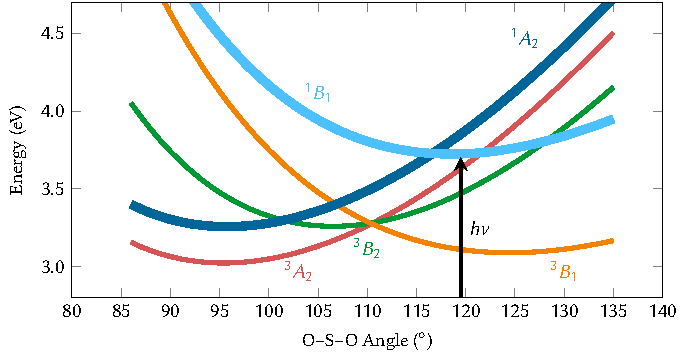
\includegraphics[width=0.9\textwidth]{img/pes/pes.pdf}
   \caption{1D PES scan along the bending angle of \ce{SO2} for the 5 relevant \textbf{diabatic} states.}\label{fig:PES_1D} 
\end{figure}
\begin{figure}[p]
  \centering
  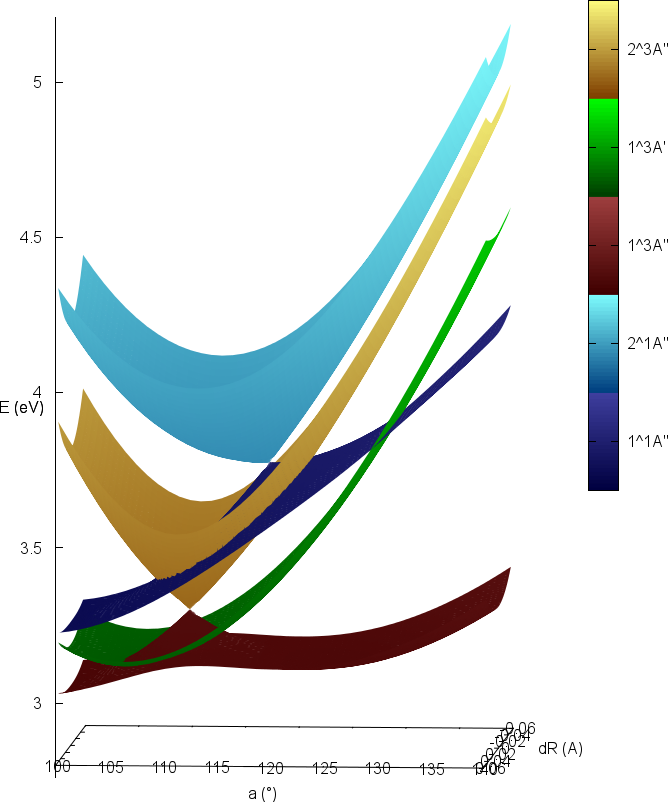
\includegraphics[height=12cm]{figures/plot_2D_trim.png}
  \caption{2D PES scan along bending angle and asymmetric stretch of \ce{SO2} for the 5 relevant \textbf{adiabatic} (but spin-diabatic) states, showing the two conical intersections between the two $^1A''$ states and between the two $^3A''$ states.}\label{fig:PES_2D}
\end{figure}







% ======================================================================================================
% ======================================================================================================
% ======================================================================================================

\chapter{Full Tutorial}\label{chap:full}
\section{Before you Start}

In this tutorial, the steps necessary to perform non-adiabatic dynamics with the \sharc\ dynamics suite using \textsc{AMS}, in particular \textsc{ADF}, are explained.
These steps include preparation tasks like optimization and frequency calculation, generation of the Wigner distribution of initial conditions, calculation of the excited states of these initial conditions, and initial state selection. 
Subsequently, it will be shown how to setup the input files for an ensemble of trajectories and how they are executed.
Furthermore, the tutorial presents some trajectory analysis steps, including plotting of energies, populations, etc.\ of a single trajectory, calculation of internal coordinates, or of ensemble populations.
Also, the setup of a parametrized LVC model is shown.

As the tutorial will produce many output files and directories, it is recommended that you work in a separate directory for it:
\begin{Verbatim}[commandchars=\\\{\}]
user@host> \textbf{\textcolor{red}{mkdir Tutorial}}
user@host> \textbf{\textcolor{red}{cd Tutorial/}}
\end{Verbatim}

\section{Important}

Beyond the core dynamics program, the \sharc\ suite contains a number of Python scripts allowing to perform various types of setup and analysis tasks. 
There are two types of these scripts.

\emph{Non-interactive scripts} can be controlled by command-line arguments and options. 
Every non-interactive script can be called with the command line option \ttt{-h} in order to get a description of the functionality and possible options.

\emph{Interactive scripts} ask the user for information about the task to be conducted (using features like auto-complete and default values), and only perform the task after the input has been completed. 

In the tutorial, the input dialogue of the interactive scripts is shown as in this example. 
\texttt{\textbf{\textcolor{red}{Red bold text}}} gives the input which the user has to type. 
\begin{oframed}
\footnotesize\begin{Verbatim}[commandchars=\\\{\}]
Type of calculation: \textbf{\textcolor{red}{2}}
Frequency calculation? [True] \textbf{\textcolor{red}{<ENTER>}}

Geometry filename: [geom.xyz] (autocomplete enabled) \textbf{\textcolor{red}{g<TAB>}}
Geometry filename: [geom.xyz] (autocomplete enabled) \textbf{\textcolor{red}{geom.xyz}}

Enter atom indices: (range comprehension enabled) \textbf{\textcolor{red}{1~4}}
\end{Verbatim}
\end{oframed}

\normalsize
During the interactive sessions, square brackets indicate that the question has a default answer, which can be used by just pressing ENTER. 
If filenames or directory paths need to be entered, auto-complete is active, which can be used by pressing TAB. 
If a list of integers (e.g., atom indices) needs to be entered, range comprehension is active, and ranges can be entered with the tilde symbol (e.g., \ttt{1\textasciitilde 4} is equivalent to \ttt{1 2 3 4}).
Upon completion, every interactive script produces a file \ttt{KEYSTROKES.<name>}, which contains all user input for the last run.

\begin{shaded}
  Please make sure before starting that \ttt{\$SHARC} is set to the directory containing the \sharc\ scripts and executables.

  It is also advisable to set \ttt{\$AMSHOME} to the \textsc{AMS} main directory.
\end{shaded}

Note that in principle one should be able to reproduce all results in this tutorial, i.e., if you closely follow the given steps then you should see exactly the same output (and the same figures).
The only exception to this is that the results might be different if you employed a different compiler to compile \ttt{sharc.x} (this tutorial uses \ttt{gfortran 4.8.5}) or if you use a different \textsc{AMS} version (this tutorial uses \textsc{AMS2020.102}).

\refermanual{m-chap:aux}
Note that it is recommended that for sections in which the user is especially interested, they should refer to the corresponding sections in the \sharc\ Manual.
The corresponding sections are indicated in margin notes on the right (see example on the right).



\clearpage
\section{Optimization and Frequency calculation}\label{tut:optfreq}

The first general step of a dynamics simulation is the setup of the initial conditions.
Here, we will sample initial conditions randomly from the ground state Wigner distribution.

In order to carry out this step, we need to prepare a \textsc{Molden} file containing the results of a frequency calculation for the ground state.
In general, the user is free to calculate the frequencies and normal modes with any quantum chemistry software and any method he sees fit, as long as a \textsc{Molden} file can be produced. 
However, usually it is advisable to calculate the frequencies at the same level of theory as the dynamics calculation. 
For sulfur dioxide in our example, we will do the frequency calculation with the quantum chemistry method specified above: (DFT PBE/DZP). 

Create an empty directory. 
Prepare an \ttt{ams.run} file to start a geometry optimization and calculation of the normal modes.
\begin{Verbatim}[commandchars=\\\{\}]
user@host> \textbf{\textcolor{red}{mkdir Opt_Freq}}
user@host> \textbf{\textcolor{red}{cd Opt_Freq}}
user@host> \textbf{\textcolor{red}{vi ams.run}}
\end{Verbatim}
If not already happened, set up your environment for the calculations with \textsc{AMS} by sourcing the \ttt{amsbashrc.sh} file from the installation folder (\ttt{\$AMSHOME})
\begin{Verbatim}[commandchars=\\\{\}]
  user@host> \textbf{\textcolor{red}{source \$AMSHOME/amsbashrc.sh}}
  \end{Verbatim}
Inside the file write the following.
\begin{oframed}
\footnotesize\begin{Verbatim}[commandchars=\\\{\}]
#!/bin/sh 
$AMSBIN/ams -n 1 << EOF 
 
Task GeometryOptimization 
Properties 
    NormalModes Yes 
End 
 
System 
    Atoms 
        O     0.      1.3      -0.65
        S     0.      0.        0.
        O     0.     -1.3      -0.65
    End 
End 
Engine ADF 
    save INFO 
    Basis 
        Type DZP 
    End 
    Relativity 
        Formalism ZORA 
        Level Scalar 
    End 
    XC
        Dispersion Grimme3 BJDAMP
        gga PBE
    End 
EndEngine
EOF
\end{Verbatim}
\end{oframed}

\normalsize

Execute the run script to start the \textsc{AMS} optimization and frequency calculation.
\begin{Verbatim}[commandchars=\\\{\}]
user@host> \textbf{\textcolor{red}{sh ams.run > AMS.log &}}
\end{Verbatim}
This will produce the file \ttt{AMS.log} and the directory \ttt{ams.results/}. 
The file contains (among other things) the ground state minimum energy (should be $-0.60471660$ Hartree) and the vibrational wavenumbers. 
Check for any imaginary frequencies.
There should be a block like this in you output.
\begin{oframed}
\footnotesize\begin{Verbatim}[commandchars=\\\{\}]

  -----------------------
  Normal Mode Frequencies
  -----------------------
 
  Index   Frequency (cm-1)   Intensity (km/mol)   Irrep
      7           486.2798              23.8004      A1
      8          1089.9122              30.1834      A1
      9          1293.5389             183.4285      B2
 
  Zero-point energy (Hartree):     0.0065
 
  ------------
  Normal Modes
  ------------
      \vdots          \vdots          \vdots          \vdots         \vdots          \vdots         \vdots          \vdots
\end{Verbatim}
\end{oframed}

\normalsize
The \ttt{ams.results/} folder contains all fragment calculations as well as the general calculation file \ttt{ams.rkf} and the engine specific binary file \ttt{adf.rkf}, which contains the normal modes next to other informations about the calculation and results. 
We will generate the \ttt{AMS.freq.molden} from the \ttt{adf.rkf} file with the help of another \sharc\ script and copy it as \ttt{AMS.freq.molden} into the Tutorial folder and change to it for the next steps.

\begin{Verbatim}[commandchars=\\\{\}]
  user@host> \textbf{\textcolor{red}{$SHARC/AMS-ADF_freq.py ams.results/adf.rkf}}
  user@host> \textbf{\textcolor{red}{cp ams.results/adf.rkf.molden ../AMS.freq.molden}}
\end{Verbatim}
Go back up to the \ttt{Tutorial} folder to continue.
\begin{Verbatim}[commandchars=\\\{\}]
user@host> \textbf{\textcolor{red}{cd ..}}
\end{Verbatim}











\clearpage
\section{Sampling initial Conditions from a Wigner distribution}
\refermanual{m-sec:wigner.py}
\refermanual{m-met:wigner}

In the next step, the initial coordinates and velocities for the trajectories have to be generated.
Here, this task is accomplished by sampling randomly from the Wigner distribution of the ground state nuclear wave function (in the harmonic approximation), which can be calculated from the vibrational frequencies and normal modes.
This task is performed by the non-interactive script \ttt{wigner.py}, which can be executed by typing
\begin{Verbatim}[commandchars=\\\{\}]
user@host> \textbf{\textcolor{red}{$SHARC/wigner.py -n 20 AMS.freq.molden}}
\end{Verbatim}
The \ttt{-n} option is necessary to specify the number of initial conditions to be generated. 
Here, we generate 20 initial conditions. 
The output should look like this:
\begin{oframed}
\footnotesize\begin{Verbatim}[commandchars=\\\{\}]
Initial condition generation started...
INPUT  file                  = "AMS.freq.molden"
OUTPUT file                  = "initconds"
Number of geometries         = 20
Random number generator seed = 16661
Temperature                  = 0.000000

***************************************************                 \textcolor{blue}{# We did not include the rigid modes}
WARNING: Less than 3*N_atom normal modes, but no [N_FREQ] keyword!  \textcolor{blue}{# as they are not needed.} 
***************************************************                 \textcolor{blue}{# You can ignore this warning.}


Starting normal mode format determination...
Final format specifier: 1 [gaussian-type (Gaussian, Turbomole, Q-Chem, ADF, Orca)]
The normal modes input format was determined to be gaussian-type (Gaussian, Turbomole, Q-Chem, ADF, Orca) 
coordinates.

Geometry:
 O   8.0   1.85081016  -0.12565904   0.05565681  15.99491500 
 S  16.0   4.61375846  -0.24577894  -0.13448766  31.97207100 
 O   8.0   5.74691718  -1.59710862  -2.27346244  15.99491500 
Assumed Isotopes: S-32 O-16 
Isotopes with * are pure isotopes.

Frequencies (cm^-1) used in the calculation:
   1     487.8300
   2    1090.7900
   3    1292.6000

Sampling initial conditions
Progress: [==================================================] 100%
\end{Verbatim}
\end{oframed}
\normalsize

The results of the sampling are written to the file \ttt{initconds}. 
This file contains all necessary information (equilibrium geometry, plus 20 sets of randomly sampled geometries with corresponding velocities) for subsequent steps.











\clearpage
\section{Setting up the initial energy calculations}
\refermanual{m-sec:typical_workflow}

Besides the initial geometries and velocities, it is necessary to determine (for each initial geometry) the initial excited state from where the dynamics commences.
In order to find the initial states after instantaneous vertical excitation, it is necessary to obtain the excitation energies and oscillator strengths for all initial geometries. 
These calculations can be setup using the script \ttt{setup\_init.py}. 

Note that it is also possible to simply specify the initial state for each initial condition manually; in this case, it is not necessary to use \ttt{setup\_init.py} to prepare vertical excitation calculations. 



\subsection{\textsc{AMS} input template}

The computations which are setup by \ttt{setup\_init.py} utilize the \sharc\ interfaces to call the respective quantum chemistry program (\textsc{AMS} here).
The \sharc-\textsc{AMS} interface requires a template file which specifies the level of theory.
Thus, before proceeding to setup the initial calculations, we need to prepare the \textsc{AMS} template file.

Again, open a file called \ttt{AMS-ADF.template}:
\begin{Verbatim}[commandchars=\\\{\}]
user@host> \textbf{\textcolor{red}{vi AMS-ADF.template}}
\end{Verbatim}
You can find a \ttt{AMS-ADF.template} file in the examples (\ttt{\$SHARC/../examples/SHARC\_AMS-ADF/AMS-ADF.template}), where we wrote every possible option that you could put in there with explanatory comments (see below).
\begin{oframed}
\footnotesize\begin{Verbatim}[commandchars=\\\{\}]
  ## This is a commented version of the AMS-ADF.template file 
  ## for version 2.1 of the SHARC_AMS-ADF.py interface.

  ## ======== BASIS SETS ============

  ## This keyword activates the relativistic Hamiltonian of ADF.
  ## If no keyword is given, a nonrelativistic calculation is done.
  ## All arguments are written verbatim to ADF input.
relativistic scalar zora

  ## This keyword defines the basis set for all atoms.
  ## Specific basis sets per element can be defined with the basis_per_element key below.
  ## Examples: SZ, DZ, DZP, TZP, TZ2P, QZ4P, ...
basis DZP

  ## This keyword sets the path to the basis set library of ADF.
  ## Bash variables and ~ are automatically expanded by the interface.
#basis_path $AMSRESOURCES

  ## This keyword overwrites the basis set from the "basis" key for a given element.
  ## The "basis_per_element" key can occur several times in the template.
  ## Requires two arguments, first the element, then the path to the basis set file (full path necessary)
  ## Can also define a basis set for an extra fragment (e.g. H.1).
#basis_per_element S $AMSRESOURCES/ZORA/DZP/S
#basis_per_element H.1 $AMSRESOURCES/ZORA/DZP/H

  ## Defines an atomic fragment for use in ADF, with labels formatted like "El.i"
  ## With the "basis_per_element" key, one can then specify basis sets for each defined fragment.
  ## The format is "define_fragment <label> <list of atom numbers>
  ## All specified atoms must be of the element given in the label.
  ## Note that in QM/MM calculations, the force field file must contain extra parameters for the element 
  ## "El.i".
# define_fragment  H.1  3 5 6



  ## ======== CHEMISTRY ============

  ## This keyword defines the XC functional.
  ## All arguments are written verbatim to ADF input.
  ## Note that for gradient calculations, only LDA, GGA, and HYBRID work
  ## See https://www.scm.com/doc/ADF/Input/Density_Functional.html#keyscheme-xc
  ## Examples for  first argument: LDA, GGA, HYBRID ( METAGGA, METAHYBRID, HartreeFock, LIBXC )
  ## Examples for second argument: VWN, Xonly, Xalpha;   BP86, PBE, PW91, ...;   B3LYP, PBE0, ...
functional gga pbe

  ## This keyword activates the XCFUN keyword in ADF, which is a library to evaluate functionals.
  ## See https://www.scm.com/doc/ADF/Input/Density_Functional.html#keyscheme-xc
#functional_xcfun

  ## This keyword activates dispersion correction.
  ## All arguments are written verbatim to ADF input.
  ## See the ADF manual for possible options.
dispersion grimme3 bjdamp

  ## This keyword sets the total charge of the molecule.
  ## For QM/MM calculations, you have to specify the charge of the QM (with link atoms replaced) only!
  ## Unlike in the ADF input, this keyword does not allow to set the number of unpaired electrons.
  ## Instead, the interface automatically sets this number based on the requested multiplicity.
  ##
  ## This keyword accepts either a single number, or as many numbers as there are multiplicities.
  ## If only one charge is given but several multiplicities requested in QM.in, then the interface
  ## will automatically check and assign the charges based on the nuclear charge (this might not for for 
  ## QM/MM).
  ## If after the "charge" keyword one charge is given for each multiplicities, these numbers will used as 
  ## is.
  ## 
  ## (for QM/MM it is advisable to always give more than one charge values to disable automatic assignment)
charge 0 +1 0 +1 0
#charge 0

  ## With this keyword, the interface returns total energies instead of bonding energies.
  ## Note that in ADF bonding energies are more accurate than total energies.
  ## Total energies are not available for relativistic or QM/MM calculations.
#totalenergy

  ## With this keyword, the interface requests a COSMO calculation in ADF, with the solvent given as 
  ## argument.
  ## COSMO is not compatible with gradient calculations.
  ## Examples of solvents: see https://www.scm.com/doc/ADF/Input/COSMO.html#keyscheme-solvation
#cosmo water

  ## This keyword activates nonequilibrium solvation for excited states.
  ## For vertical excitation calculations, this value should be the square of the refraction index of the 
  ## solvent.
  ## If you neglect this keyword, ADF will assume equilibrium solvation (incorrect for vertical 
  ## excitations).
#cosmo_neql 1.77

  ## use the full adiabatic XC kernel for excited states. Default is to use ALDA.
  ## Cannot be combined with gradients
#fullkernel



  ## ======== ACCURACY and CONVERGENCE ============

  ## This keyword controls the integration grid.
  ## One can either use the modern Becke grid (ADF>=2013) or the older Voronoi grid.
  ## For Becke, use: (normal is often sufficient, you may also you good)
grid beckegrid normal     # Options: basic, normal, good, verygood, excellent
  ## For Voronoi, use:
#grid integration 4.0    # Options: 4.0, 5.0, 6.0, ...

  ## This keyword controls the integration grid generation around MM point charges.
  ## grids are only generated for MM charges closer than this distance to any QM atom.
  ## It only has any effect in QM/MM runs, but it works for both Becke and Voronoi grids.
  ## The default is 7.5589 Bohr (equal to 4 Angstrom).
#grid_qpnear 7.5589

  ## With this keyword, the integration grid quality can be controlled per atom.
  ## This keyword can occur several times, where later lines overwrite earlier lines.
  ## Atoms which are not mentioned are treated with the quality given with the grid keyword.
  ## Note that MM point charges cannot be affected with this keyword, use the grid keyword instead.
  ## Has no effect if the Voronoi grid is used.
#grid_per_atom good 1 2 3
#grid_per_atom basic 4 5 6

  ## This keyword sets the Coulomb fitting scheme.
  ## One can either use the modern ZlmFit (ADF>=2013) or the older STOFit.
  ## For ZlmFit, use:
fit zlmfit normal         # Options: basic, normal, good, verygood, excellent
  ## For STOFit, use:
#fit stofit

  ## With this keyword, the ZlmFit quality can be controlled per atom.
  ## This keyword can occur several times, where later lines overwrite earlier lines.
  ## Atoms which are not mentioned are treated with the quality given with the fit keyword.
  ## Has no effect if the STOfit is used.
#fit_per_atom verygood 1
#fit_per_atom good 2 3

  ## This keyword activates the "exactdensity" keyword in the ADF input.
  ## ADF will then use the exact electron density for the XC potential.
  ## See the ADF manual for more details.
#exactdensity

  ## This keyword activates the use of the new HF exchange scheme.
  ## The default is to not use the new scheme.
  ## The new scheme might be faster and better parallelized, but benchmarking is advisable.
  ## It can only be used with functionals that have HF exchange
  ## Note that energies (SCF+Davidson) usually take much longer than gradients (CPKS+integration).
#rihartreefock normal     # Options: basic, normal, good, verygood, excellent

  ## With this keyword, the rihartreefock quality can be controlled per atom.
  ## This keyword can occur several times, where later lines overwrite earlier lines.
  ## Atoms which are not mentioned are treated with the quality given with the rihartreefock keyword.
  ## Has no effect if rihartreefock is not used.
#rihf_per_atom verygood 1
#rihf_per_atom good 2 3

  ## This keyword places the occupations keyword (not as block) into the ADF input.
  ## All arguments are copied verbatim to the input.
  ## See the ADF manual for more details.
#occupations keeporbitals=50

  ## This sets the number of SCF cycles (the interface will use 100 by default).
scf_iterations 200

  ## This activates the "linearscaling" option of ADF.
  ## By default, this option is not used in the ADF input.
  ## The argument is a number between 0 and 99, where values <8 are sloppier, >8 are tighter than default.
#linearscaling 8

  ## This sets the convergence threshold for the CPKS equations (for excited-state gradients)
cpks_eps 0.0001



  ## ======== EXCITATIONS ============

  ## This keyword deactivates TDA (which the interface will request by default).
#no_tda

  ## This keyword increases the number of excited states for the Davidson step.
  ## These extra states will not be reported in the output, which is controlled by the "states" request in 
  ## QM.in.
  ## Like the "charges" key, padding can be specified per multiplicity.
  ## Note that extra states change how the Davidson procedure converges and thus can slightly affect the 
  ## results.
paddingstates 1 0 0 0 0

  ## Sets the number of davidson vectors.
  ## The default is to let ADF decide on the number of vectors (this gives min(40,nstates+40) ).
  ## For optimal performance, might be increased to around 5*nstates.
dvd_vectors 60

  ## Sets the davidson tolerance (difference in excitation energies between iterations).
  ## Default is 1e-6.
dvd_tolerance 1e-6

  ## Sets the davidson residual tolerance (norm of the residual vectors).
  ## Can significantly accelerate the Davidson procedure (if set to ~sqrt(dvd_tolerance) or slightly below).
  ## Default is the same value as dvd_tolerance.
dvd_residu 1e-3

  ## This keyword activates the "MBLOCKSMALL" keyword in the ADF input.
  ## Without the "MBLOCKSMALL" keyword, ADF's updates multiple states in each iteration, possibly even 
  ## converged ones.
  ## With the "MBLOCKSMALL" keyword, states are updated one by one, skipping already converged ones and 
  ## thus being faster.
  ## Recommendation: Using "dvd_mblocksmall" will give shorter runtimes, but in some situations convergence 
  ## might be signalled before all states are actually fully converged.
#dvd_mblocksmall

  ## This keyword requests that triplet states are calculated in a separate job based on an open-shell 
  ## triplet ground state.
  ## The default is that triplets are calculated based on the closed-shell singlet ground state.
  ## Unrestricted triplets are not compatible with a spin-orbit computation.
#unrestricted_triplets

  ## This activates the "modifyexcitations" keyword in the ADF input.
  ## The option can be used to compute core excitation states (e.g., for X-Ray spectra).
  ## It takes a single argument.
  ## For example, "modifyexcitations 5" means that excitations are only allowed out of the 5 lowest MOs.
#modifyexcitations 5

## ===============================================================================================
## For those familiar with ADF input files, here some infos what the interface does automatically:
## ===============================================================================================
##
## SYSTEM block with units: always Bohr, input geometry is converted appropriately.
## Atoms block: nuclear coordinates of the molecule.

## SYMMETRY keyword: always uses nosym
##
## CHARGE keyword: automatically uses the correct charge per multiplicity and n_alpha-n_beta
##
## UNRESTRICTED keyword: placed if necessary (for all but singlet ground state)

## Within the ENGINE block:

## BASIS block: automatically sets "core none", "createoutput none"
##
## EXCITATIONS block: always "davidson", automatically uses "onlysing", "onlytrip", "lowest", and requests 
## different numbers of singlets/triplets.
##
## SOPERT keyword: automatic, if SOC requested and triplets present
##
## GSCORR keyword: automatic, if singlets and triplets present
##
## GRADIENT keyword: Uses this undocumented keyword in place of a GEOMETRY block
##
## EXCITEDGO block: Used automatically, cpks eps is always set to 0.0001, sing_grads/trip_grads are used 
##
## SAVE keyword: saves TAPE21, and TAPE15 for overlap and Dyson calculations
##
## DEPENDENCY keyword: is always added
##
## NOPRINT keyword: "logfile", if the interface does not run in debug mode.
##
## RESTART keyword: used to restart the MOs from the last/present time step, or from initial MOs
##
## QMMM block: always uses NEWQMMM, output_level=1, warning_level=1, optimize(method skip) for gradients
##
## SHARCOVERLAP keyword: uses this undocumented keyword to compute the AO-overlap matrix for neighboring 
## geometries.
##
\end{Verbatim}
\end{oframed}

However, you only need to type the following into your \ttt{AMS-ADF.template} file.
\begin{oframed}
  \begin{Verbatim}[commandchars=\\\{\}]
relativistic scalar zora 
basis DZP
functional gga pbe
dispersion grimme3 bjdamp
charge 0 +1 0
scf_iterations 200
cpks_eps 0.0001
paddingstates 1 0 0
dvd_vectors 60
dvd_tolerance 1e-6
dvd_residu 1e-3
  \end{Verbatim}
\end{oframed}

\normalsize
Save the file and continue to the next section.

\clearpage
\subsection{Setup of initial calculations}
\refermanual{m-sec:molcas_input.py}

With the necessary files (\ttt{initconds}, \ttt{AMS-ADF.template}) available, the script \ttt{setup\_init.py} can be launched.
Note that this script creates a large number of subdirectories in the directory where the script is run, so it is advisable to run the setup in a dedicated directory:
\begin{Verbatim}[commandchars=\\\{\}]
user@host> \textbf{\textcolor{red}{mkdir init/}}
user@host> \textbf{\textcolor{red}{cd init/}}
user@host> \textbf{\textcolor{red}{$SHARC/setup_init.py}}
\end{Verbatim}
This script is also interactive. 

\begin{oframed}
\footnotesize\begin{Verbatim}[commandchars=\\\{\}]


  ================================================================================
||                                                                                ||
||                     Setup trajectories for SHARC dynamics                      ||
||                                                                                ||
||                    Authors: Sebastian Mai, Severin Polonius                    ||
||                                                                                ||
||                                  Version: 2.1                                  ||
||                                 Date: 01.09.19                                 ||
||                                                                                ||
  ================================================================================


This script automatizes the setup of excited-state calculations for initial conditions
for SHARC dynamics.
  
-------------------Initial conditions file------------------


If you do not have an initial conditions file, prepare one with wigner.py!

Please enter the filename of the initial conditions file.
Initial conditions filename: [initconds] (autocomplete enabled) \textbf{\textcolor{red}{../initconds}}

File "../initconds" contains 20 initial conditions.
Number of atoms is 3

-----------------Range of initial conditions----------------

Please enter the range of initial conditions for which an excited-state calculation should be performed as 
two integers separated by space.
Initial condition range: [1 20] \textbf{\textcolor{red}{1 10}}

Script will use initial conditions 1 to 10 (10 in total).

----------------------Number of states----------------------

Please enter the number of states as a list of integers
e.g. 3 0 3 for three singlets, zero doublets and three triplets.
Number of states: \textbf{\textcolor{red}{3  0  3}}

Number of states: [3, 0, 3]
Total number of states: 12

-----------Choose the quantum chemistry interface-----------

Please specify the quantum chemistry interface (enter any of the following numbers):
1	MOLPRO (only CASSCF)
2	COLUMBUS (CASSCF, RASSCF and MRCISD), using SEWARD integrals
3	Analytical PESs
4	MOLCAS (CASSCF, CASPT2, MS-CASPT2)
5	AMS-ADF (DFT, TD-DFT)
6	TURBOMOLE (ricc2 with CC2 and ADC(2))
7	LVC Hamiltonian
8	GAUSSIAN (DFT, TD-DFT)
9	ORCA (DFT, TD-DFT, HF, CIS)
10	BAGEL (CASSCF, CASPT2, (X)MS-CASPT2)

Interface number: \textbf{\textcolor{red}{5}}
The used interface will be: AMS-ADF (DFT, TD-DFT)

-----------------Spin-orbit couplings (SOCs)----------------

Do you want to compute spin-orbit couplings?

Spin-Orbit calculation? [True] \textbf{\textcolor{red}{<ENTER>}} 
Will calculate spin-orbit matrix.


----------------Overlaps to reference states----------------

Do you want to compute the overlaps between the states at the equilibrium geometry 
and the states at the initial condition geometries?
Reference overlaps? [False] \textbf{\textcolor{red}{yes}}    \textcolor{blue}{# not required, but included anyways.}

---------------TheoDORE wave function analysis--------------

Do you want to run TheoDORE to obtain one-electron descriptors for the electronic wave functions?
TheoDORE? [False] \textbf{\textcolor{red}{<ENTER>}} 

================================================================================
||                               AMS Interface setup                              ||
  ================================================================================


-------------------------Path to AMS------------------------

Setup from amsbashrc.sh file? [True] \textbf{\textcolor{red}{<ENTER>}}

Please specify path to the amsbashrc.sh file (SHELL variables and ~ can be used, will be expanded when 
interface is started).

Path to amsbashrc.sh file: [$AMSHOME/amsbashrc.sh] (autocomplete enabled) \textbf{\textcolor{red}{<ENTER>}} 

----------------------Scratch directory---------------------

Please specify an appropriate scratch directory. This will be used to temporally store the integrals. 
The scratch directory will be deleted after the calculation. Remember that this script cannot check 
whether the path is valid, since you may run the calculations on a different machine. 
The path will not be expanded by this script.
Path to scratch directory: (autocomplete enabled) \textbf{\textcolor{red}{$TMPDIR/Tutorial/Init}}

-------------------AMS input template file------------------

Please specify the path to the AMS-ADF.template file. This file must contain the following keywords:

basis <basis>
functional <type> <name>
charge <x> [ <x2> [ <x3> ...] ]

The AMS interface will generate the appropriate AMS input automatically.

Template filename: (autocomplete enabled) \textbf{\textcolor{red}{../AMS-ADF.template}}

------------------Initial restart: MO Guess-----------------

Please specify the path to an AMS rkf engine file (e.g., adf.rfk) containing suitable starting MOs for the 
AMS calculation. Please note that this script cannot check whether the wavefunction file and the Input 
template are consistent!

Do you have a restart file? [True] \textbf{\textcolor{red}{no}} 

-------------------AMS Ressource usage-------------------

Please specify the number of CPUs to be used by EACH calculation.

Number of CPUs: \textbf{\textcolor{red}{1}}  \textcolor{blue}{# \ce{SO2} is so small that multiple CPUs will not accelerate the computation notably.}

-----------------------WFoverlap setup----------------------

Path to wavefunction overlap executable: [$SHARC/wfoverlap.x] (autocomplete enabled) \textbf{\textcolor{red}{<ENTER>}}

State threshold for choosing determinants to include in the overlaps
For hybrids (and without TDA) one should consider that the eigenvector X may have a norm larger than 1
Threshold: [0.998] \textbf{\textcolor{red}{<ENTER>}} 

Memory for wfoverlap (MB): [1000] \textbf{\textcolor{red}{500}}

  ================================================================================
||                                 Run mode setup                                 ||
  ================================================================================


-------------------------Run script-------------------------

This script can generate the run scripts for each initial condition in two modes:

  - In mode 1, the calculation is run in subdirectories of the current directory.

  - In mode 2, the input files are transferred to another directory (e.g. a local scratch directory), the 
  calculation is run there, results are copied back and the temporary directory is deleted. Note that this 
  temporary directory is not the same as the "scratchdir" employed by the interfaces.

Note that in any case this script will create the input subdirectories in the current working directory.

In case of mode 1, the calculations will be run in:
/user/severin/workdir/ams_sharc_tutorial2/Tutorial/init

Use mode 1 (i.e., calculate here)? [True] \textbf{\textcolor{red}{<ENTER>}}     \textcolor{blue}{# this is now the default}

----------------------Submission script---------------------

During the setup, a script for running all initial conditions sequentially in batch mode is generated. 
Additionally, a queue submission script can be generated for all initial conditions.

Generate submission script? [False] \textbf{\textcolor{red}{<ENTER>}}


#########################Full input#########################

ninit                      20
natom                      3
initf                      <_io.TextIOWrapper name='../initconds' mode='r' encoding='UTF-8'>
irange                     [1, 10]
states                     [3, 0, 3]
nstates                    12
interface                  5
needed                     ['wfoverlap']
soc                        True
refov                      True
theodore                   False
cwd                        /user/severin/workdir/ams_sharc_tutorial2/Tutorial/init
amsbashrc                  /usr/license/adf/ams2020.102/amsbashrc.sh
ams                        $AMSHOME
scmlicense                 $SCMLICENSE
scratchdir                 $TMPDIR/Tutorial/Init
AMS-ADF.template               ../AMS-ADF.template
ams.guess                  \{\}
ams.ncpu                   1
ams.scaling                0.9
ams.wfoverlap              $SHARC/wfoverlap.x
ams.ciothres               0.998
ams.mem                    500
here                       True
qsub                       False

Do you want to setup the specified calculations? [True] \textbf{\textcolor{red}{<ENTER>}}


  ================================================================================
||                            Setting up directories...                           ||
  ================================================================================


Progress: [==================================================] 100%
\end{Verbatim}
\end{oframed}

\normalsize
The script will create directories \ttt{ICOND\_00001/}, \ttt{ICOND\_00002/}, ... for each initial condition (and \ttt{ICOND\_00000/} for the equilibrium geometry), with the corresponding inputs for the interface and a Bash runscript. 
Additionally, the script \ttt{all\_run\_init.sh} is generated, which allows to run all excited-state calculations subsequently. 

Run all initial conditions calculations sequentially:
\begin{Verbatim}[commandchars=\\\{\}]
user@host> \textbf{\textcolor{red}{sh all_run_init.sh}}
\end{Verbatim}
For larger calculations, it is often advantageous to send the scripts \ttt{ICOND\_*/run.sh} to a queueing system to distribute the calculations over a computing cluster.
However, note that with the \ttt{reference overlap} calculations, \ttt{ICOND\_00000} must be completed before you can send the other calculations.

After the calculations are finished, each subdirectory should contain a file called \ttt{QM.out} holding the Hamiltonian and transition dipole moment matrices.







\clearpage
\section{Selection of initial excited states}
\refermanual{m-sec:excite.py}
\refermanual{m-met:exc_selection}

In the next step, the results of the excited-state calculations have to be read, converted to excitation energies and oscillator strengths, and the brightest initial conditions selected for the dynamics simulation.
These tasks can be accomplished using 
\begin{Verbatim}[commandchars=\\\{\}]
user@host> \textbf{\textcolor{red}{$SHARC/excite.py}}
\end{Verbatim}

This script is interactive. 
Per default, during the run the script reads the ground state equilibrium energy from \ttt{ICOND\_00000/QM.out}, if this file exists. 
Otherwise, the script asks the user to enter the ground states equilibrium energy.

\begin{oframed}
\footnotesize\begin{Verbatim}[commandchars=\\\{\}]
  ================================================================================
||                                                                                ||
||                       Excite initial conditions for SHARC                      ||
||                                                                                ||
||                              Author: Sebastian Mai                             ||
||                                                                                ||
||                                   Version:2.1                                  ||
||                                    01.09.19                                    ||
||                                                                                ||
  ================================================================================


This script automatizes to read-out the results of initial excited-state calculations for SHARC.
It calculates oscillator strength (in MCH and diagonal basis) and stochastically determines whether
a trajectory is bright or not.
  
-------------------Initial conditions file------------------


If you do not have an initial conditions file, prepare one with wigner.py!

Please enter the filename of the initial conditions file.
Initial conditions filename: [initconds] (autocomplete enabled) \textbf{\textcolor{red}{../initconds}}

File "../initconds" contains 20 initial conditions.
Number of atoms is 6

----------------Generate excited state lists----------------

Using the following options, excited state lists can be added to the initial conditions:

1       Generate a list of dummy states
2       Read excited-state information from ab initio calculations (from setup_init.py)

How should the excited-state lists be generated? [2] \textbf{\textcolor{red}{<ENTER>}}     \textcolor{blue}{# Read from ICOND_*/}
Please enter the path to the directory containing the ICOND subdirectories.
Path to ICOND directories: (autocomplete enabled) \textbf{\textcolor{red}{.}}            \textcolor{blue}{# "." is the current directory}

/user/mai/Documents/NewSHARC/SHARC_2.0/TUTORIAL/2_full/Tutorial/init
Directory contains 11 subdirectories.
There are more initial conditions in ../initconds.

----------------Excited-state representation----------------

This script can calculate the excited-state energies and oscillator strengths in two representations.
These representations are:
- MCH representation: Only the diagonal elements of the Hamiltonian are taken into account. 
The states are the spin-free states as calculated in the quantum chemistry code. 
This option is usually sufficient for systems with small SOC (below 300 cm^-1).
- diagonal representation: The Hamiltonian including spin-orbit coupling is diagonalized. 
The states are spin-corrected, fully adiabatic. Note that for this the excited-state calculations 
have to include spin-orbit couplings. This is usually not necessary for systems with small SOC.

Do you want to use the diagonal representation (yes=diag, no=MCH)? \textbf{\textcolor{red}{no}}


----------------------Reference energy----------------------

Reference energy read from file 
/user/mai/Documents/NewSHARC/SHARC_2.0/TUTORIAL/2_full/Tutorial/init/ICOND_00000/QM.out
E_ref=-0.600159310000      \textcolor{blue}{# automatically read from ICOND_00000/QM.out}


-------------------Excited-state selection------------------

Using the following options, the excited states can be flagged as valid initial states for dynamics:

1       Unselect all initial states
2       Provide a list of desired initial states
3       Simulate delta-pulse excitation based on excitation energies and oscillator strengths

How should the excited states be flagged? [3] \textbf{\textcolor{red}{<ENTER>}}


----------------------Excitation window---------------------

Enter the energy window for exciting the trajectories.
Range (eV): [0.0 10.0] \textbf{\textcolor{red}{3  6}}

Script will allow excitations only between 3.000000 eV and 6.000000 eV.

----------------------Considered states---------------------

From which state should the excitation originate (for computation of excitation energies 
and oscillator strength)?
Lower state for excitation? [1] \textbf{\textcolor{red}{<ENTER>}}
#State  Mult    M_s     Quant    \textcolor{blue}{# Here the states are listed.}
1       1      +0.0     1
2       1      +0.0     2
3       1      +0.0     3
4       3      -1.0     1
5       3      -1.0     2
6       3      -1.0     3
7       3      +0.0     1
8       3      +0.0     2
9       3      +0.0     3
10      3      +1.0     1
11      3      +1.0     2
12      3      +1.0     3

Do you want to include all states in the selection? [True] \textbf{\textcolor{red}{<ENTER>}}

---------------------Random number seed---------------------

Please enter a random number generator seed (type "!" to initialize the RNG from the system time).
RNG Seed:  [!] \textbf{\textcolor{red}{1234}}



#########################Full input#########################

initf                      <open file '../initconds', mode 'r' at 0x7f6df7fcd660>
eharm                      0.0
ninit                      20
diag                       False
erange                     [0.11024792647342582, 0.22049585294685164]
allowed                    set([])
excite                     3
repr                       MCH
states                     [3, 0, 3]
ion                        False
iconddir                   /user/severin/workdir/ams_sharc_tutorial2/Tutorial/init
make_list                  False
eref                       -0.60015931
ncond                      11
natom                      3
read_QMout                 True
initstate                  0
diabatize                  False
gen_list                   2

Do you want to continue? [True] \textbf{\textcolor{red}{<ENTER>}}

Reading initial condition file ....
  Progress: [==================================================] 100%
Number of initial conditions in file:          20

Reading QM.out data ...
  Progress: [==================================================] 100%
Number of initial conditions with QM.out:      10

Selecting initial states ...
  Progress: [==================================================] 100%
Number of initial states:                       6

Number of initial conditions excited:
State   Selected   InRange   Total
    1          0         0      10
    2          6        10      10     \textcolor{blue}{# we can setup 6 trajectories from state 2 (S1)}
    3          0        10      10
    4          0         6      10
    5          0        10      10
    6          0        10      10
    7          0         6      10
    8          0        10      10
    9          0        10      10
   10          0         6      10
   11          0        10      10
   12          0        10      10
Writing output to ../initconds.excited ...
\end{Verbatim}
\end{oframed}

\normalsize

\ttt{excite.py} will generate a new file called \ttt{initconds.excited}, which contains all information from the \ttt{initconds} file, as well as information about the ground state equilibrium energy, the state representation and the excited states for each initial condition. 
This file is necessary in order to calculate absorption spectra and to setup trajectories.

If you later want to do another selection (with a different excitation window or with the exclusion of some states), you can tell \ttt{excite.py} to read from \ttt{initconds.excited}, instead of reading all \ttt{QM.out} files again. 

From the \ttt{initconds.excited} file, also absorption spectra can be generated, see section~\ref{sec:absspec}.
If you do not want to compute a spectrum and directly go to the trajectory setup, go to section~\ref{sec:setup_traj}.






\clearpage
\section{Absorption spectra from Initial conditions files}\label{sec:absspec}
\refermanual{m-sec:spectrum.py}
\refermanual{m-met:spectrum}

The content of the file \ttt{initconds.excited} can be used to generate absorption spectra which go beyond the Condon approximation. The spectrum is the sum of the spectra of each initial condition, which is a line spectrum of the excitation energies versus the oscillator strengths. A Gaussian (or Lorentzian, or Log-normal) convolution of the line spectra can be done as well.

The calculation of convoluted or line spectra is carried out by \ttt{spectrum.py}. 

\subsection{Example}

Call the script by
\begin{Verbatim}[commandchars=\\\{\}]
user@host> \textbf{\textcolor{red}{cd ..}}
user@host> \textbf{\textcolor{red}{$SHARC/spectrum.py -o spectrum.out -e 3 6 initconds.excited}}
\end{Verbatim}
Using command-line options, it is possible to calculate only spectra for part of the initial condition set, to change the size and limits of the energy grid (here we plot from 3 eV to 6 eV) and to influence the line shape (Gaussian vs.\ Lorentzian vs.\ Log-normal, as well as FWHM). With the \ttt{-l} option a line spectrum is produced, and with the \ttt{-D} option a density-of-states spectrum is produced.

The program also writes some information about the calculation to the screen:
\begin{oframed}
\footnotesize\begin{Verbatim}[commandchars=\\\{\}]
  Number of grid points: 500
  Energy range: 3.000 to 6.000 eV
  Lineshape: Gaussian (FWHM=0.100 eV)
  Number of initial conditions: 20
  Reference energy    -0.6001593100
  Representation: MCH
  Reading initial conditions 1 to 20
  
  Progress: [=========================                         ]  50%
  
  Number of states: 12
  Number of initial conditions with excited-state information (per state):
  10 10 10 10 10 10 10 10 10 10 10 10 
  
  Progress: [==================================================] 100%
  
  Maximum of the absorption spectrum: 0.018224
  
  Output spectrum written to "spectrum.out".
\end{Verbatim}
\end{oframed}

\normalsize
The results can be easily plotted using \textsc{Gnuplot}. Just give the corresponding command-line flag and then call \textsc{Gnuplot}:
\begin{Verbatim}[commandchars=\\\{\}]
user@host> \textbf{\textcolor{red}{$SHARC/spectrum.py -o spectrum.out -e 3 6}}
           \textbf{\textcolor{red}{--gnuplot spectrum.gp initconds.excited}}
user@host> \textbf{\textcolor{red}{gnuplot spectrum.gp}}
\end{Verbatim}

In figure~\ref{fig:spectrum} (\ttt{spectrum.out.png}) the result of this convolution is shown.
Note that the strucuture of the spectrum is misleading, since classical nuclei do not allow the computation of vibrational structure.

\begin{figure}[h]
  \centering
  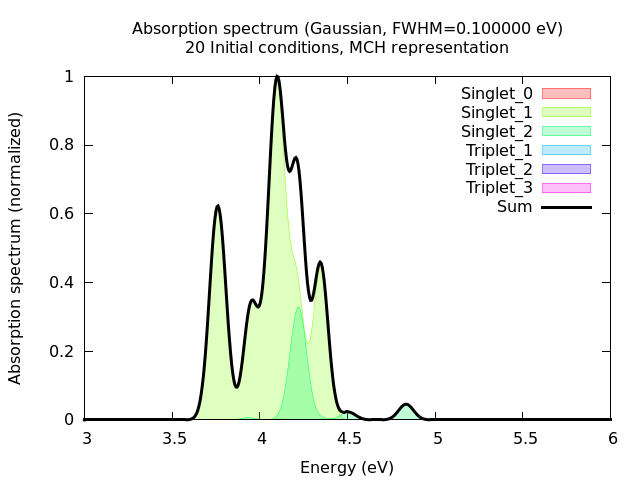
\includegraphics[width=0.75\textwidth]{figures/spectrum.png}
  \caption{Absorption spectrum of \ce{SO2} based on 10 initial conditions (Since there are 20 initial conditions in \ttt{initconds.excited}, the title lists 20 instead of 10).}
  \label{fig:spectrum}
\end{figure}











\clearpage
\section{Setting up dynamics simulations}\label{sec:setup_traj}
\refermanual{m-sec:setup_traj.py}

The last preparatory step towards dynamics simulations consists naturally in setting up the \sharc\ input files and run scripts. 
The interactive script \ttt{setup\_traj.py} takes care of this step. 
Run the script in the directory where the trajectories should be set up. 
For this, create a new directory:
\begin{Verbatim}[commandchars=\\\{\}]
user@host> \textbf{\textcolor{red}{mkdir traj}}
user@host> \textbf{\textcolor{red}{cd traj}}
\end{Verbatim}
Make sure that you have all required files (\ttt{initconds.excited}, \ttt{AMS-ADF.template}) in this directory.
Then start the setup script:
\begin{Verbatim}[commandchars=\\\{\}]
user@host> \textbf{\textcolor{red}{$SHARC/setup_traj.py}}
\end{Verbatim}

\begin{oframed}
\footnotesize\begin{Verbatim}[commandchars=\\\{\}]
  ================================================================================
||                                                                                ||
||                     Setup trajectories for SHARC dynamics                      ||
||                                                                                ||
||          Authors: Sebastian Mai, Philipp Marquetand, Severin Polonius          ||
||                                                                                ||
||                                  Version: 2.1                                  ||
||                                 Date: 01.09.19                                 ||
||                                                                                ||
  ================================================================================


This script automatizes the setup of the input files for SHARC dynamics.
  

  ================================================================================
||                               Initial conditions                               ||
  ================================================================================



This script reads the initial conditions (geometries, velocities, initial excited state)
from the initconds.excited files as provided by excite.py.

Please enter the filename of the initial conditions file.
Initial conditions filename: [initconds.excited] (autocomplete enabled) \textbf{\textcolor{red}{../initconds.excited}}

File ../initconds.excited contains 20 initial conditions.
Number of atoms is 3
Reference energy -0.600159310000 a.u.
Excited states are in MCH representation.


Please enter the number of states as a list of integers
e.g. 3 0 3 for three singlets, zero doublets and three triplets.
Number of states: [3 0 3] \textbf{\textcolor{red}{<ENTER>}}        \textcolor{blue}{# a different number of states than in the}
                                         \textcolor{blue}{# initial calculations could be used in the dynamics}

Number of states: [3, 0, 3]
Total number of states: 12

Do you want all states to be active? [True] \textbf{\textcolor{red}{<ENTER>}}

Do you want to see the content of the initconds file? [True] \textbf{\textcolor{red}{<ENTER>}}
Number of initial conditions in file:          20
Contents of the initconds file:

Legend:
?       Geometry and Velocity
.       not selected
#       selected

State 1:
             10         20         30         40         50         60         70         80         90         
             100
              |          |          |          |          |          |          |          |          |          
              |
 0 | .......... ?????????? 
State 2:
             10         20         30         40         50         60         70         80         90         
             100
              |          |          |          |          |          |          |          |          |          
              |
 0 | .####.#..# ?????????? 
State 3:
             10         20         30         40         50         60         70         80         90         
             100
              |          |          |          |          |          |          |          |          |          
              |
 0 | .......... ?????????? 
State 4:
             10         20         30         40         50         60         70         80         90         
             100
              |          |          |          |          |          |          |          |          |          
              |
 0 | .......... ?????????? 
State 5:
             10         20         30         40         50         60         70         80         90         
             100
              |          |          |          |          |          |          |          |          |          
              |
 0 | .......... ?????????? 
State 6:
             10         20         30         40         50         60         70         80         90         
             100
              |          |          |          |          |          |          |          |          |          
              |
 0 | .......... ?????????? 
State 7:
             10         20         30         40         50         60         70         80         90         
             100
              |          |          |          |          |          |          |          |          |          
              |
 0 | .......... ?????????? 
State 8:
             10         20         30         40         50         60         70         80         90         
             100
              |          |          |          |          |          |          |          |          |          
              |
 0 | .......... ?????????? 
State 9:
             10         20         30         40         50         60         70         80         90         
             100
              |          |          |          |          |          |          |          |          |          
              |
 0 | .......... ?????????? 
State 10:
             10         20         30         40         50         60         70         80         90         
             100
              |          |          |          |          |          |          |          |          |          
              |
 0 | .......... ?????????? 
State 11:
             10         20         30         40         50         60         70         80         90         
             100
              |          |          |          |          |          |          |          |          |          
              |
 0 | .......... ?????????? 
State 12:
             10         20         30         40         50         60         70         80         90         
             100
              |          |          |          |          |          |          |          |          |          
              |
 0 | .......... ?????????? 
Number of excited states and selections:
State    #InitCalc       #Selected
    1           10               0
    2           10               6
    3           10               0
    4           10               0
    5           10               0
    6           10               0
    7           10               0
    8           10               0
    9           10               0
   10           10               0
   11           10               0
   12           10               0

Please enter a list specifying for which excited states trajectories should be set-up
e.g. 5 7 12 to select states 5, 7, and 12.
States to setup the dynamics: [2] (range comprehension enabled) \textbf{\textcolor{red}{<ENTER>}}

There can be 6 trajectories set up.

Please enter the index of the first initial condition in the initconds file to be setup.
Starting index: [1] \textbf{\textcolor{red}{<ENTER>}}

There can be 6 trajectories set up, starting in 1 states.

Please enter the total number of trajectories to setup.
Number of trajectories: [6] \textbf{\textcolor{red}{<ENTER>}}

Please enter a random number generator seed (type "!" to initialize the RNG from the system time).
RNG Seed:  [!] \textbf{\textcolor{red}{1234}}


  ================================================================================
||                     Choose the quantum chemistry interface                     ||
  ================================================================================


Please specify the quantum chemistry interface (enter any of the following numbers):
1       MOLPRO (only CASSCF)
2       COLUMBUS (CASSCF, RASSCF and MRCISD), using SEWARD integrals
3       Analytical PESs
4       MOLCAS (CASSCF, CASPT2, MS-CASPT2)
5       AMS (DFT, TD-DFT)
6       TURBOMOLE (ricc2 with CC2 and ADC(2))
7       LVC Hamiltonian
8       GAUSSIAN (DFT, TD-DFT)
9       ORCA (DFT, TD-DFT, HF, CIS)
10      BAGEL (CASSCF, CASPT2, (X)MS-CASPT2)

Interface number: \textbf{\textcolor{red}{5}}
The used interface will be: AMS (DFT, TD-DFT)

  ================================================================================
||                        Surface Hopping dynamics settings                       ||
  ================================================================================


-----------------------Simulation time----------------------

Please enter the total simulation time.
Simulation time (fs): [1000.0] \textbf{\textcolor{red}{100}}

Please enter the simulation timestep (0.5 fs recommended).
Simulation timestep (fs): [0.5] \textbf{\textcolor{red}{<ENTER>}}

Simulation will have 201 timesteps.

Please enter the number of substeps for propagation (25 recommended).
Nsubsteps: [25] \textbf{\textcolor{red}{<ENTER>}}

The trajectories can be prematurely terminated after they run for a certain time in the lowest state. 
Do you want to prematurely terminate trajectories? [False] \textbf{\textcolor{red}{<ENTER>}}


----------------------Dynamics settings---------------------

Do you want to perform the dynamics in the diagonal representation (SHARC dynamics) 
or in the MCH representation (regular surface hopping)?
SHARC dynamics? [True] \textbf{\textcolor{red}{<ENTER>}}
Do you want to include spin-orbit couplings in the dynamics?

Spin-Orbit calculation? [True] \textbf{\textcolor{red}{<ENTER>}}
Will calculate spin-orbit matrix.


Please choose the quantities to describe non-adiabatic effects between the states:
1       DDT     =  < a|d/dt|b >        Hammes-Schiffer-Tully scheme   (not available)
2       DDR     =  < a|d/dR|b >        Original Tully scheme          (not available)
3       overlap = < a(t0)|b(t) >       Local Diabatization scheme     
Coupling number: [3] \textbf{\textcolor{red}{<ENTER>}}

For SHARC dynamics, the evaluation of the mixed gradients necessitates to calculate 
non-adiabatic coupling vectors (Extra computational cost).
... but interface cannot provide non-adiabatic coupling vectors, turning option off.

During a surface hop, the kinetic energy has to be modified in order to conserve total energy. 
There are several options to that:
1       Do not conserve total energy. Hops are never frustrated.
2       Adjust kinetic energy by rescaling the velocity vectors. Often sufficient.
3       Adjust kinetic energy only with the component of the velocity vector along 
        the non-adiabatic coupling vector.        (not possible)
4       Adjust kinetic energy only with the component of the velocity vector along
        the gradient difference vector.
EkinCorrect: [2] \textbf{\textcolor{red}{<ENTER>}}

If a surface hop is refused (frustrated) due to insufficient energy, the velocity can either be 
left unchanged or reflected:
1       Do not reflect at a frustrated hop.
2       Reflect the full velocity vector.
3       Reflect only the component of the velocity vector along the non-adiabatic coupling vector.
        (not possible)
4       Reflect only the component of the velocity vector along the gradient difference vector.
Reflect frustrated: [1] \textbf{\textcolor{red}{<ENTER>}}

Please choose a decoherence correction for the diagonal states:
1       No decoherence correction.
2       Energy-based decoherence scheme (Granucci, Persico, Zoccante).
3       Augmented fewest-switching surface hopping (Jain, Alguire, Subotnik).
Decoherence scheme: [2] \textbf{\textcolor{red}{<ENTER>}}

Please choose a surface hopping scheme for the diagonal states:
1       Surface hops off.
2       Standard SHARC surface hopping probabilities (Mai, Marquetand, Gonzalez).
3       Global flux surface hopping probabilities (Wang, Trivedi, Prezhdo).
Hopping scheme: [2] \textbf{\textcolor{red}{<ENTER>}}

Do you want to perform forced hops to the lowest state based on a energy gap criterion?
(Note that this ignores spin multiplicity)
Forced hops to ground state? [False] \textbf{\textcolor{red}{<ENTER>}}

Do you want to scale the energies and gradients?
Scaling? [False] \textbf{\textcolor{red}{<ENTER>}}

Do you want to damp the dynamics (Kinetic energy is reduced at each timestep by a factor)?
Damping? [False] \textbf{\textcolor{red}{<ENTER>}}

Do you want to use an atom mask for velocity rescaling or decoherence?
Atom masking? [False] \textbf{\textcolor{red}{<ENTER>}}

---------------Selection of Gradients and NACs--------------

In order to speed up calculations, SHARC is able to select which gradients and NAC vectors it has to 
calculate at a certain timestep. The selection is based on the energy difference between the state 
under consideration and the classical occupied state.

Select gradients? [False] \textbf{\textcolor{red}{yes}}    \textcolor{blue}{# this strongly speeds up the calculations}

Please enter the energy difference threshold for the selection of gradients and non-adiabatic 
couplings (in eV). (0.5 eV recommended, or even larger if SOC is strong in this system.)
Selection threshold (eV): [0.5] \textbf{\textcolor{red}{0.1}}


-------------------------Laser file-------------------------

Do you want to include a laser field in the simulation? [False] \textbf{\textcolor{red}{<ENTER>}}

---------------TheoDORE wave function analysis--------------

Do you want to run TheoDORE to obtain one-electron descriptors for the electronic wave functions?
TheoDORE? [False] \textbf{\textcolor{red}{<ENTER>}} 

  ================================================================================
||                               AMS Interface setup                              ||
  ================================================================================


-------------------------Path to AMS------------------------

Setup from amsbashrc.sh file? [True] \textbf{\textcolor{red}{<ENTER>}}

Please specify path to the amsbashrc.sh file (SHELL variables and ~ can be used, will be expanded when 
interface is started).

Path to amsbashrc.sh file: [$AMSHOME/amsbashrc.sh] (autocomplete enabled) \textbf{\textcolor{red}{<ENTER>}}

----------------------Scratch directory---------------------

Please specify an appropriate scratch directory. This will be used to temporally 
store the integrals. The scratch directory will be deleted after the calculation. 
Remember that this script cannot check whether the path is valid, since you may 
run the calculations on a different machine. The path will not be expanded by this script.
Path to scratch directory: (autocomplete enabled) \textbf{\textcolor{red}{$TMPDIR/Tutorial/Traj_WORK/}}

-------------------AMS input template file------------------

Please specify the path to the AMS-ADF.template file. This file must contain the following keywords:

basis <basis>
functional <type> <name>
charge <x> [ <x2> [ <x3> ...] ]

The AMS interface will generate the appropriate AMS input automatically.

Template filename: (autocomplete enabled) \textbf{\textcolor{red}{../AMS-ADF.template}}

------------------Initial restart: MO Guess-----------------

Please specify the path to an AMS engine file (e.g. adf.rkf) containing suitable starting MOs for the 
AMS calculation. 
Please note that this script cannot check whether the wavefunction file and the Input template are 
consistent!

Do you have a restart file? [True] \textbf{\textcolor{red}{no}}
WARNING: Remember that the calculations may take longer without an initial guess for the MOs.
---------------------AMS Ressource usage--------------------

Please specify the number of CPUs to be used by EACH calculation.

Number of CPUs: \textbf{\textcolor{red}{1}} 

--------------------Wfoverlap code setup--------------------

Path to wavefunction overlap executable: [$SHARC/wfoverlap.x] (autocomplete enabled) \textbf{\textcolor{red}{<ENTER>}

State threshold for choosing determinants to include in the overlaps
For hybrids (and without TDA) one should consider that the eigenvector X may have a norm larger than 1
Threshold: [0.998] \textbf{\textcolor{red}{<ENTER>}}

Memory for wfoverlap (MB): [1000] \textbf{\textcolor{red}{500}}

  ================================================================================
||                           Content of output.dat files                          ||
  ================================================================================


SHARC or PYSHARC can produce output in ASCII format (all features supported currently)
or in NetCDF format (more efficient file I/O, some features currently not supported).
Write output in NetCDF format? [False] \textbf{\textcolor{red}{<ENTER>}}

Do you want to write the gradients to the output.dat file?
Write gradients? [False] \textbf{\textcolor{red}{<ENTER>}}

Do you want to write the non-adiabatic couplings (NACs) to the output.dat file?
Write NACs? [False] \textbf{\textcolor{red}{<ENTER>}}

Do you want to write property matrices to the output.dat file  (e.g., Dyson norms)?
Write property matrices? [False] \textbf{\textcolor{red}{<ENTER>}}

Do you want to write property vectors to the output.dat file  (e.g., TheoDORE results)?
Write property vectors? [False] \textbf{\textcolor{red}{<ENTER>}}

Do you want to write the overlap matrix to the output.dat file ?
Write overlap matrix? [True] \textbf{\textcolor{red}{<ENTER>}}

Do you want to modify the output.dat writing stride?
Modify stride? [False] \textbf{\textcolor{red}{<ENTER>}}


  ================================================================================
||                                 Run mode setup                                 ||
  ================================================================================


-------------------------Run script-------------------------

This script can generate the run scripts for each trajectory in two modes:

  - In the first mode, the calculation is run in subdirectories of the current directory.

  - In the second mode, the input files are transferred to another directory (e.g. a local scratch 
  directory), the calculation is run there, results are copied back and the temporary directory is 
  deleted. Note that this temporary directory is not the same as the scratchdir employed by the interfaces.

Note that in any case this script will setup the input subdirectories in the current working directory.

In case of mode 1, the calculations will be run in:
/user/mai/Documents/NewSHARC/SHARC_2.1/TUTORIAL/traj

Use mode 1 (i.e., calculate here)? [True] \textbf{\textcolor{red}{<ENTER>}}

----------------------Submission script---------------------

During the setup, a script for running all initial conditions sequentially in batch mode is generated. 
Additionally, a queue submission script can be generated for all initial conditions.

Generate submission script? [False] \textbf{\textcolor{red}{<ENTER>}}


#########################Full input#########################

ninit                      20
natom                      3
repr                       MCH
diag                       False
eref                       -0.60015931
eharm                      0.0
initf                      <_io.TextIOWrapper name='../initconds.excited' mode='r' encoding='UTF-8'>
states                     [3, 0, 3]
nstates                    12
statemap                   {1: [1, 1, 0.0], 2: [1, 2, 0.0], 3: [1, 3, 0.0], 4: [3, 1, -1.0], 5: [3, 2, -1.0], 
                           6: [3, 3, -1.0], 7: [3, 1, 0.0], 8: [3, 2, 0.0], 9: [3, 3, 0.0], 10: [3, 1, 1.0], 11: [3, 2, 1.0],
                           12: [3, 3, 1.0]}
actstates                  [3, 0, 3]
isactive                   [True, True, True, True, True, True, True, True, True, True, True, True]
show_content               True
n_issel                    [0, 6, 0, 0, 0, 0, 0, 0, 0, 0, 0, 0]
setupstates                {2}
firstindex                 1
ntraj                      6
interface                  5
needed                     ['wfoverlap']
tmax                       100.0
dtstep                     0.5
nsubstep                   25
kill                       False
surf                       diagonal
soc                        True
coupling                   3
phases_from_interface      False
gradcorrect                False
ekincorrect                2
reflect                    1
decoherence                ['edc', '0.1']
hopping                    sharc
force_hops                 False
force_hops_dE              9999.0
scaling                    False
damping                    False
atommaskarray              []
sel_g                      True
sel_t                      False
eselect                    0.1
laser                      False
dipolegrad                 False
ion                        False
theodore                   False
amsbashrc                  /usr/license/adf/ams2020.102/amsbashrc.sh
ams                        $AMSHOME
scmlicense                 $SCMLICENSE
scratchdir                 $TMPDIR/Tutorial/Traj_WORK/
AMS-ADF.template               ../AMS-ADF.template
ams.guess                  \{\}
ams.ncpu                   1
ams.scaling                0.9
ams.wfoverlap              $SHARC/wfoverlap.x
ams.ciothres               0.998
ams.mem                    500
pysharc                    False
netcdf                     False
write_grad                 False
write_NAC                  False
write_property2d           False
write_property1d           False
write_overlap              True
stride                     [1]
printlevel                 2
cwd                        /user/severin/workdir/ams_sharc_tutorial2/Tutorial/traj
here                       True
copydir                    /user/severin/workdir/ams_sharc_tutorial2/Tutorial/traj
qsub                       False

Do you want to setup the specified calculations? [True] \textbf{\textcolor{red}{<ENTER>}}


  ================================================================================
||                            Setting up directories...                           ||
  ================================================================================


Progress: [==================================================] 100%

6 trajectories setup, last initial condition was 10 in state 2.
\end{Verbatim}
\end{oframed}

\normalsize

The script creates for each of the initial states (``States to setup the dynamics'') a directory called \ttt{<Mult>\_<Num>}, e.g., \ttt{Singlet\_1/}, which contains the input for all trajectories starting in that state. 
Each of these directories contains subdirectories named \ttt{TRAJ\_00001/}, \ttt{TRAJ\_00002/}, etc. 
Note that these numbers are not consecutive: if an initial condition has not been selected, the number will be missing.
Each subdirectory contains the \sharc\ input (consisting of the files \ttt{input}, \ttt{geom}, and \ttt{veloc}), the directories \ttt{QM/} and \ttt{restart/}, and the run script for the trajectory, \ttt{run.sh}.

For the purposes of the tutorial it is sufficient to only calculate one trajectory. Change to the subdirectory of one of the trajectories and execute it.
\begin{Verbatim}[commandchars=\\\{\}]
user@host> \textbf{\textcolor{red}{cd Singlet_1/TRAJ_00002}}
user@host> \textbf{\textcolor{red}{sh run.sh&}}
user@host> \textbf{\textcolor{red}{tail -f output.lis}}
\end{Verbatim}
While the trajectory is running, you can watch its progress in the file \ttt{output.lis} (short output listing). For each timestep, it contains the currently occupied diagonal state (and approximate MCH state), the kinetic, potential and total energy, the RMS gradient, the state dipole and spin expectation values of the currently occupied diagonal state and the time needed for this step. Surface hopping events are also mentioned in this file.

Besides the \ttt{output.lis} file, \sharc\ creates the files \ttt{output.log}, \ttt{output.xyz} and \ttt{output.dat}. 
The file
\ttt{output.log} contains mainly parsing information of the input file parsing and a list of internal steps of the dynamics simulation. 
With sufficiently high \ttt{printlevel} in the \sharc\ input file, the log file may also contain debug information in various detail, but with the default setting, no relevant information is printed.
The file \ttt{output.dat} contains for each timestep the most important matrices and vectors. 
This information can be used to calculate the excited-state energies, populations, hopping probabilities and a large number of expectation values. 
See below for the usage of \ttt{data\_extractor.x} and \ttt{make\_gnuplot.py}, which can be used for plotting the mentioned quantities.
Finally, \ttt{output.xyz} contains the cartesian coordinates of all atoms for each timestep. 
This file can be opened with any program capable of processing xyz files, like \textsc{Molden}, \textsc{Molekel} and \textsc{Gabedit}. 
Additionally, the geometries can be analyzed with the programs \ttt{geo.py}, which is a command line tool to extract internal coordinates from such an xyz file, \ttt{trajana\_nma.py}, and \ttt{trajana\_essdyn.py}.



% ===========================================================================================================================
% ===========================================================================================================================
% ===========================================================================================================================

\clearpage
\section{Analyzing a single trajectory}

We will first discuss the analysis of a single trajectory based on the output files. 
Later (section~\ref{sec:analyze_ensemble}) we will also analyze ensemble properties. 

If you are not in the directory for the trajectory \ttt{TRAJ\_00002/}, change to this directory:
\begin{Verbatim}[commandchars=\\\{\}]
user@host> \textbf{\textcolor{red}{cd Singlet_2/TRAJ_00002}}
\end{Verbatim}


% ======================================================================================================

\subsection{Data extraction and plotting}
\refermanual{m-sec:data_extractor.x}
\refermanual{m-sec:make_gnuscript.py}

The file \ttt{output.dat} contains the Hamiltonian, transformation matrix, dipole matrices, coefficients, hopping probabilities, kinetic energy and random number from the surface hopping procedure in a compressed form. The program \ttt{data\_extractor.x} can be used to generate data tables, which can then be plotted.
\begin{Verbatim}[commandchars=\\\{\}]
user@host> \textbf{\textcolor{red}{$SHARC/data_extractor.x output.dat}}
\end{Verbatim}
The program creates a subdirectory called \ttt{output\_data/}. With the default settings, the following files will be created:
\begin{itemize}
  \item \ttt{coeff\_diab.out}, \ttt{coeff\_class\_diab.out}, \ttt{coeff\_mixed\_diab.out} contain the coefficients and populations in the diabatic representation (only approximate).
  \item \ttt{coeff\_diag.out}, \ttt{coeff\_class\_diag.out}, \ttt{coeff\_mixed\_diag.out} contain the coefficients and populations in the diagonal representation.
  \item \ttt{coeff\_MCH.out}, \ttt{coeff\_class\_MCH.out}, \ttt{coeff\_mixed\_MCH.out} contain the coefficients and populations in the MCH representation.
  \item \ttt{energy.out} contains kinetic, current potential, total and potential energy of all excited states.
  \item \ttt{fosc.out} contains the oscillator strengths of the current state and all excited states.
  \item \ttt{fosc\_act.out} contains the oscillator strengths of all states relative to the active state.
  \item \ttt{spin.out} contains the total spin expectation values of the current state and all excited states.
  \item \ttt{prob.out} contains the surface hopping random number and the hopping probabilities in the diagonal representation.
  \item \ttt{expec.out} contains the content of \ttt{energy.out}, \ttt{fosc.out} and \ttt{spin.out} in one file (for plotting).
  \item \ttt{expec\_MCH.out} is analogue to \ttt{expec.out}, except all data is given in the MCH representation (except the active state energy).
\end{itemize}

In order to plot the content of these files in an efficient manner, \ttt{gnuplot} can be used. Use
\begin{Verbatim}[commandchars=\\\{\}]
user@host> \textbf{\textcolor{red}{$SHARC/make_gnuscript.py  3  0  3 > plot.gp}}
\end{Verbatim}
to create a \ttt{gnuplot} script with the correct state numbering and labeling. Execute
\begin{Verbatim}[commandchars=\\\{\}]
user@host> \textbf{\textcolor{red}{gnuplot plot.gp}}
\end{Verbatim}
to plot energies, populations and hopping probabilities (Use \textbf{\textcolor{red}{\ttt{<ENTER>}}} to continue with the next plot). In figures~\ref{fig:en}, \ref{fig:cMCH}, \ref{fig:cDIAG} and~\ref{fig:prob} the output for trajectory \ttt{TRAJ\_00002/} for the first 100~fs is given.


\begin{figure}[tb]
  \centering
  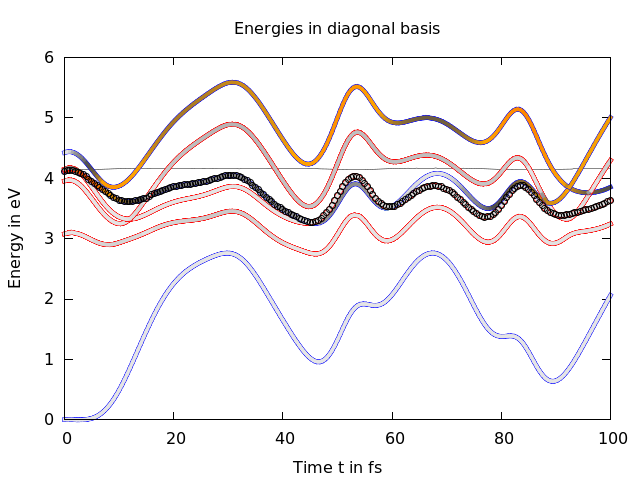
\includegraphics[width=\textwidth]{figures/energy.png}
  \caption{Plot of the potential energies for trajectory \ttt{TRAJ\_00002/} with 3 singlet and 3 triplet states.}
  \label{fig:en}
\end{figure}
\begin{figure}[tb]
  \centering
  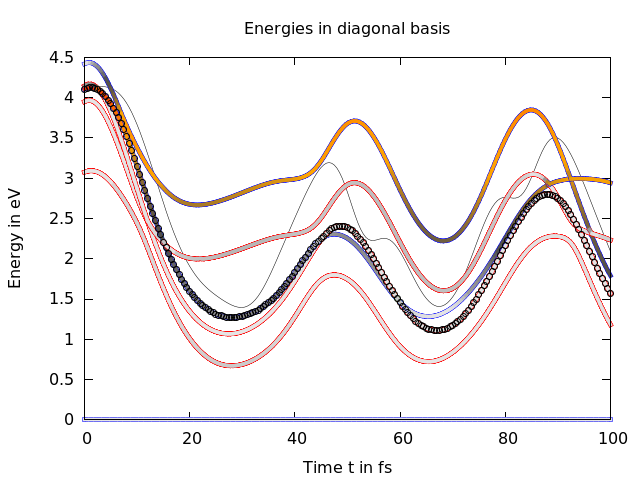
\includegraphics[width=\textwidth]{figures/energy_rel.png}
  \caption{Plot of the \emph{relative} potential energies for trajectory \ttt{TRAJ\_00002/} with 3 singlet and 3 triplet states.  }
  \label{fig:en_rel}
\end{figure}
\begin{figure}[p]
  \centering
  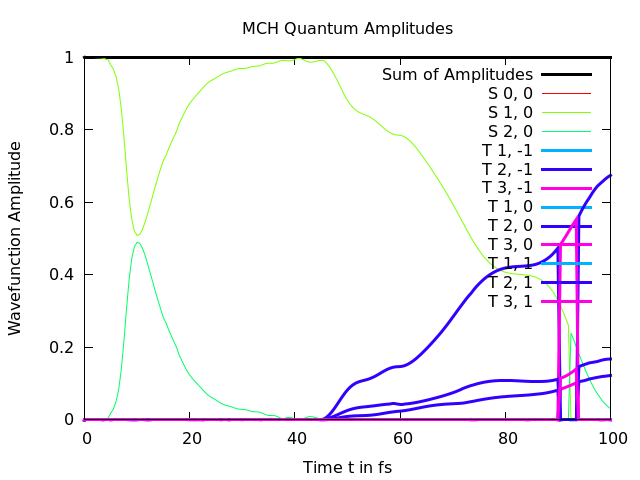
\includegraphics[width=0.95\textwidth]{figures/coeff_MCH.png}
  \caption{Plot of the excited-state populations in the MCH representation.}
  \label{fig:cMCH}
\end{figure}
\begin{figure}[p]
  \centering
  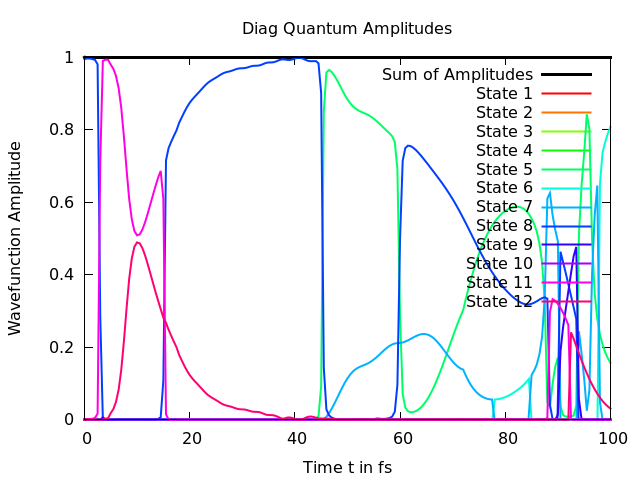
\includegraphics[width=0.95\textwidth]{figures/coeff_diag.png}
  \caption{Plot of the excited-state populations in the diagonal representation.}
  \label{fig:cDIAG}
\end{figure}
\begin{figure}[p]
  \centering
  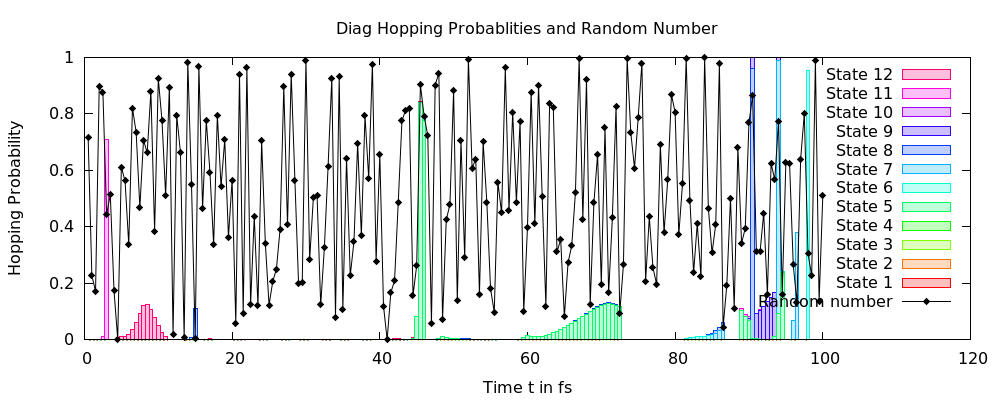
\includegraphics[width=0.95\textwidth]{figures/prob.png}
  \caption{Plot of the hopping probabilities in the diagonal representation. Additionally, the random number for the surface hopping procedure is given.}
  \label{fig:prob}
\end{figure}

\paragraph{Discussion of Figure~\ref{fig:en}}

In figure~\ref{fig:en}, the potential energies of all states included in the dynamics depending on time is given. 
The total energy is given by the thin black line (around 4~eV) and the currently occupied state is marked with black circles. 
Each state is represented by a line that is colored in two ways, with an inner core color and an outer colored contour.
The inner color encodes the oscillator strength of the state at each instant of time. 
Dark states are \textcolor{black!20}{light grey}, while brighter states are given in \textcolor{black!40}{grey}, \textcolor{black!70}{dark grey}, \textcolor{red!60!green}{orange}, \textcolor{red}{red}, \textcolor{red!50!blue}{magenta} or \textcolor{blue}{blue}, in order of increasing oscillator strength. 
The outer color encodes the total spin expectation value. 
Singlets are \textcolor{blue}{blue}, triplets \textcolor{red}{red} and states with mixed singlet-triplet character are \textcolor{green!90!black}{green}. 

In the figure, the trajectory starts in the bright singlet state slightly above 4~eV (the $S_1$).
The ground state (grey/blue line), the $T_1$ and $T_2$ (grey/red lines) are at lower energies, whereas the $T_3$ (grey/red line) and the $S_2$ (red/blue line) are at higher energies.
In the figure, there are multiple hopping events with six after 86~fs (see the \ttt{output.lis} file for all hoppings and timestamps).
It can be seen that the trajectory stays within the $S_1$ state until it hops to the $T_2$ state at 45~fs. 
The system stays in this state although crossing with the $S_1$ at 60~fs. It later hops to the $T_3$ and back at 86~fs and 96~fs, respectively.

In our case, the total energy is stable and well-behaved. If there would be some inconsistencies, that can have different reasons (e.g., wrong gradients, too large time steps, convergence problems). The small inconsistencies with the total energies in this case (slight changes) indicate that the gradient selection threshold that is too loose. 

Ultimately, the user is responsible to check the trajectories for such problematic time steps.
Note that this trajectory checking can also be carried out while the trajectories are still running; if a problematic trajectory is encountered, it can be terminated gracefully by creating an empty file called \ttt{STOP} in the run directory of that trajectory.

\paragraph{Discussion of Figure~\ref{fig:en_rel}}

In figure~\ref{fig:en_rel}, the same data as in figure~\ref{fig:en} is presented, the only difference being that in figure~\ref{fig:en_rel} all energies are relative to the energy of the lowest state.
This is often useful if there are strong oscillations in the energies of all states that make it difficult to see the energy gaps between the states.

Note that in this plot, the grey line represents the difference between total energy and energy of the lowest state, and hence does not need to be a straight line.

\paragraph{Discussion of Figure~\ref{fig:cMCH}}

In figure~\ref{fig:cMCH}, the MCH populations are given depending on time. 
The system starts with 100\% of the population in the $S_1$. 
Around 5~fs, the population is increasingly transferred to the $S_2$ up to almost 50\%. 
From this point, as no hop occured, the decoherence correction that is employed in the computation is forcing the population into the $S_1$ again.
Then, at 45~fs population flows consistently to the $T_2$ with all three magnetic quantum numbers until the end of the simulation. 
There are two very fast population transfers between the $T_2$ and the $T_3$ state and back in the end, which is an unavoided crossing of the uncoupled ${}^3B_2$ and ${}^3B_1$ states. 
These fast transfers can be explained with the crossings that are visible in figure~\ref{fig:en} and \ref{fig:en_rel}.
It is therefore generally instructive to observe the correlation between the population transfers in figure~\ref{fig:cMCH} with the hopping events in figure~\ref{fig:en}.


\paragraph{Discussion of Figure~\ref{fig:cDIAG}}

In figure~\ref{fig:cDIAG}, the diagonal populations are given depending on time. 
The difference between the MCH and diagonal populations is due to the fact that the diagonal states are strictly ordered according to energy.
This can be seen best in the second half of the figure, where population is occasionally exchanged (with 100\% efficiency).
%These population transfers happen where the $S_0$ and $T_1$ states cross (e.g., before the crossing the $S_0$ is lower than $T_1$ and hence $S_0$ is state 1. After the crossing, $S_0$ becomes state 4, and the population is transferred to state 4 to conserve the spin multiplicity of the total wave function).

Note that in this more complicated case, the diagonal populations are of little use for interpretation purposes, so that most users will prefer to analyze the MCH populations.


\paragraph{Discussion of Figure~\ref{fig:prob}}

Figure~\ref{fig:prob} shows the surface hopping probabilities and the corresponding random numbers depending on time.
In a nutshell, a surface hop happens whenever the random number lies within one of the colored bars. 
The color of the bar corresponds to the state into which the trajectory will hop. 
In the diagram, there are several hopping probabilities close to unity (especially at the end). 
This corresponds to the near-complete population transfer during the unavoided crossing of states. 


% ======================================================================================================

\clearpage
\subsection{Analyzing internal coordinates}
\refermanual{m-sec:geo.py}
\refermanual{m-met:geo}

The file \ttt{output.xyz} contains the cartesian coordinates of all timesteps. 
Oftens, one is interested in the variation of certain internal coordinates (like bond lengths, angles, etc.) during the dynamics. 
The \sharc\ tool \ttt{geo.py} can quickly calculate these values. 
Invoke the program and enter the internal coordinate specifications:
\begin{Verbatim}[commandchars=\\\{\}]
  user@host> \textbf{\textcolor{red}{$SHARC/geo.py -g output.xyz -t 0.5 > Geo.out}}
\end{Verbatim}
\begin{oframed}
\footnotesize\begin{Verbatim}[commandchars=\\\{\}]
Enter the internal coordinate specifications:
\textbf{\textcolor{red}{r 1 2}}
\textbf{\textcolor{red}{r 3 2}}
\textbf{\textcolor{red}{a 1 2 3}}
\textbf{\textcolor{red}{end}}
Number of internal coordinate requests:   2
Number of geometries:    200
FINISHED!
\end{Verbatim}
\end{oframed}

\normalsize
The \ttt{-g} option specifies the filename of the input xyz geometry file, while the \ttt{-t} option specifies the timestep.

\end{Verbatim}
The file \ttt{Geo.out} contains a table with the specified internal coordinates:
\begin{oframed}
\footnotesize\begin{Verbatim}[commandchars=\\\{\}]
#                  1|                   2|                   3|                   4|
#               time|             r  1  2|             r  3  2|          a  1  2  3|
              0.0000               1.4666               1.4647             121.1881 
              0.5000               1.4643               1.4641             121.1223
              1.0000               1.4629               1.4642             121.0364
              1.5000               1.4623               1.4652             120.9306
              2.0000               1.4625               1.4671             120.8051
              2.5000               1.4636               1.4698             120.6605
              3.0000               1.4656               1.4734             120.4969
              3.5000               1.4683               1.4776             120.3085
              4.0000               1.4718               1.4827             120.1043
              4.5000               1.4760               1.4884             119.8859

                    \vdots              \vdots               \vdots                \vdots
\end{Verbatim}
\end{oframed}

Use \textsc{Gnuplot} to plot this table. 
\begin{Verbatim}[commandchars=\\\{\}]
user@host> \textbf{\textcolor{red}{gnuplot}}
\end{Verbatim}
The file \ttt{Geo.out} contains a table with the specified internal coordinates:
\begin{oframed}
\footnotesize\begin{Verbatim}[commandchars=\\\{\}]
gnuplot> \textbf{\textcolor{red}{p "Geo.out" u 1:2 w l, "Geo.out" u 1:3 w l}}     \textcolor{blue}{# Plot column 2 and 3 versus 1}
gnuplot> \textbf{\textcolor{red}{p "Geo.out" u 1:4 w l}}     \textcolor{blue}{# Plot column 4 versus 1}
\end{Verbatim}
\end{oframed}

\normalsize
The results are shown in figures \ref{fig:so} and \ref{fig:so_angle}.

\paragraph{Discussion of the internal coordinates} 

In figures~\ref{fig:so} the \ce{SO} bond length is plotted over time. It can be easily seen that after the vibrations of the molecule is dominated by the asymmetric streching of the of the two \ce{SO} bonds. The \ce{OSO} bond angle seems to change its frequency after the transition to the triplet states, as the bond angle increases faster after 60~fs than it decreased before.

\begin{figure}[htb]
  \centering
  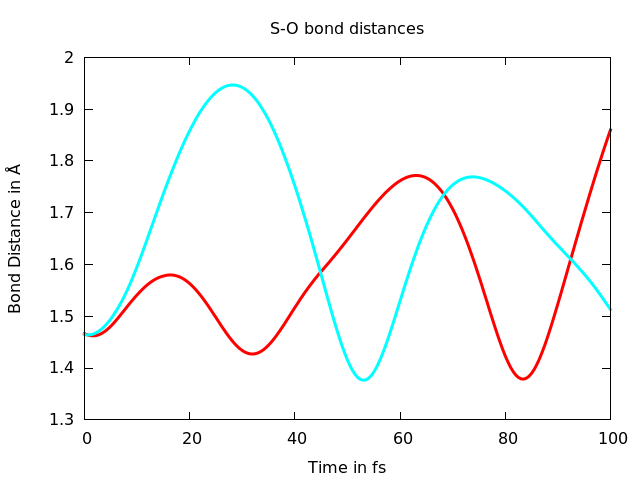
\includegraphics[width=0.8\textwidth]{figures/SO.png}
  \caption{Value of the \ce{SO} bond length during the simulation.}
  \label{fig:so}
\end{figure}

\begin{figure}[htb]
  \centering
  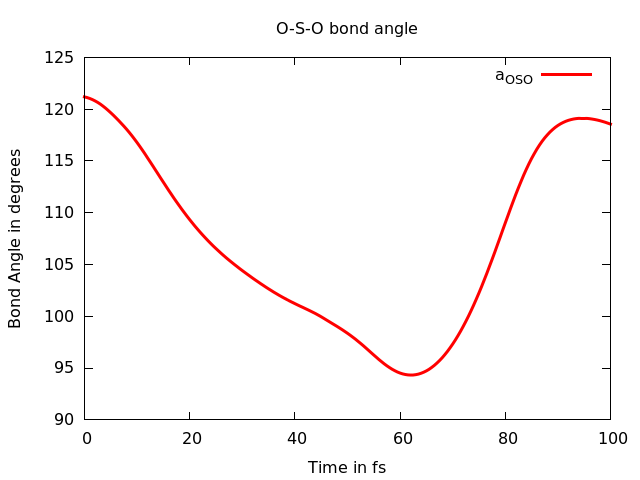
\includegraphics[width=0.8\textwidth]{figures/SO_angle.png}
  \caption{Value of the \ce{OSO} angle during the simulation.}
  \label{fig:so_angle}
\end{figure}

In order to confirm these findings, it is recommended that you load \ttt{output.xyz} into \textsc{Molden} (or another program) to watch the trajectory as a movie.







% ======================================================================================================

\clearpage
\section{Analyzing the Ensemble}\label{sec:analyze_ensemble}

For these analysis the tutorial assumes that you ran all six trajectories (\ttt{TRAJ\_00002/} to \ttt{TRAJ\_00010/}).

\subsection{Ensemble Diagnostics}
\refermanual{m-sec:diagnostics.py}

It is always a good idea to inspect the trajectories before starting with the ensemble analysis, because within the large ensemble it might not be possible to spot problems of a single trajectory.
There are two ways to inspect the trajectories---either manually checking them as described above, or the ensemble diagnostics tool, \ttt{diagnostics.py}.
This script performs a number of sanity checks for all trajectories (file existence, consistency, energy conservation, intruder states), and allows automatically marking problematic trajectories to exclude them from the analysis steps.

If you are still in the directory \ttt{TRAJ\_00002/}, go back to the root directory of the ensemble.
Then, execute \ttt{diagnostics.py}:
\begin{Verbatim}[commandchars=\\\{\}]
user@host> \textbf{\textcolor{red}{cd ../..}}
user@host> \textbf{\textcolor{red}{$SHARC/diagnostics.py}}
\end{Verbatim}


\begin{oframed}
\footnotesize\begin{Verbatim}[commandchars=\\\{\}]
  ================================================================================
||                                                                                ||
||              Diagnostic tool for trajectories from SHARC dynamics              ||
||                                                                                ||
||                              Author: Sebastian Mai                             ||
||                                                                                ||
||                                   Version:2.1                                  ||
||                                    01.09.19                                    ||
||                                                                                ||
  ================================================================================


This script reads output.dat files from SHARC trajectories and checks:
* missing files
* normal termination
* total energy conservation
* total population conservation
* discontinuities in potential and kinetic energy
  
--------------------Paths to trajectories-------------------

Please enter the paths to all directories containing the "TRAJ_0XXXX" directories.
E.g. Sing_2/ and Sing_3/. 
Please enter one path at a time, and type "end" to finish the list.
Path:  [end] (autocomplete enabled) \textbf{\textcolor{red}{Singlet_1/}}
['TRAJ_00002', 'TRAJ_00003', 'TRAJ_00004', 'TRAJ_00005', 'TRAJ_00007', 'TRAJ_00010']
Found 6 subdirectories in total.

Path:  [end] (autocomplete enabled) \textbf{\textcolor{red}{<ENTER>}}

Total number of subdirectories: 6

---------------------Diagnostic settings--------------------

Please, adjust the diagnostic settings according to your preferences.
You can use the following commands:
show            Prints the current settings
help            Prints explanations for the keys
end             Save and continue
<key> <value>   Adjust setting.

Current settings:
        missing_output : True
       missing_restart : True
    normal_termination : True
         always_update : False
           etot_window : 0.2
             etot_step : 0.1
             epot_step : 0.7
             ekin_step : 0.7
            pop_window : 1e-07
            hop_energy : 1.0
             intruders : True
        extractor_mode : default

?  [end] \textbf{\textcolor{red}{<ENTER>}}
#########################Full input#########################

paths                      ['Singlet_2/']
settings                   \{'missing_restart': True, 
                            'etot_step': 0.1, 
                            'hop_energy': 1.0, 
                            'epot_step': 0.7, 
                            'ekin_step': 0.7, 
                            'intruders': True, 
                            'pop_window': 1e-07, 
                            'missing_output': True, 
                            'normal_termination': True, 
                            'etot_window': 0.2\}

Do you want to do the specified analysis? [True] \textbf{\textcolor{red}{<ENTER>}}

Checking the directories...
~~~~~~~~~~~~~~~~~~~~~~~~~~~~~ Singlet_1/TRAJ_00002 ~~~~~~~~~~~~~~~~~~~~~~~~~~~~~

    Output files:     .lis .. .log .. .dat .. .xyz .. OK
    Restart files:    ctrl .. traj .. restart/ ..     OK
    Progress:         [=========================]     100.0 of 100.0 fs
    Status:                                           FINISHED
    Data extractor...                                 OK
    Energy:                                           OK
    Population:                                       OK
    Intruder states:                                  OK



~~~~~~~~~~~~~~~~~~~~~~~~~~~~~ Singlet_1/TRAJ_00003 ~~~~~~~~~~~~~~~~~~~~~~~~~~~~~

    Output files:     .lis .. .log .. .dat .. .xyz .. OK
    Restart files:    ctrl .. traj .. restart/ ..     OK
    Progress:         [=========================]     100.0 of 100.0 fs
    Status:                                           FINISHED
    Data extractor...                                 OK
    Energy:                                           OK
    Population:                                       OK
    Intruder states:                                  OK



~~~~~~~~~~~~~~~~~~~~~~~~~~~~~ Singlet_1/TRAJ_00004 ~~~~~~~~~~~~~~~~~~~~~~~~~~~~~

    Output files:     .lis .. .log .. .dat .. .xyz .. OK
    Restart files:    ctrl .. traj .. restart/ ..     OK
    Progress:         [=========================]     100.0 of 100.0 fs
    Status:                                           FINISHED
    Data extractor...                                 OK
    Energy:                                           OK
    Population:                                       OK
    Intruder states:                                  OK



~~~~~~~~~~~~~~~~~~~~~~~~~~~~~ Singlet_1/TRAJ_00005 ~~~~~~~~~~~~~~~~~~~~~~~~~~~~~

    Output files:     .lis .. .log .. .dat .. .xyz .. OK
    Restart files:    ctrl .. traj .. restart/ ..     OK
    Progress:         [=========================]     100.0 of 100.0 fs
    Status:                                           FINISHED
    Data extractor...                                 OK
    Energy:                                           OK
    Population:                                       OK
    Intruder states:                                  OK



~~~~~~~~~~~~~~~~~~~~~~~~~~~~~ Singlet_1/TRAJ_00007 ~~~~~~~~~~~~~~~~~~~~~~~~~~~~~

    Output files:     .lis .. .log .. .dat .. .xyz .. OK
    Restart files:    ctrl .. traj .. restart/ ..     OK
    Progress:         [=========================]     100.0 of 100.0 fs
    Status:                                           FINISHED
    Data extractor...                                 OK
    Energy:                                           OK
    Population:                                       OK
    Intruder states:                                  OK



~~~~~~~~~~~~~~~~~~~~~~~~~~~~~ Singlet_1/TRAJ_00010 ~~~~~~~~~~~~~~~~~~~~~~~~~~~~~

    Output files:     .lis .. .log .. .dat .. .xyz .. OK
    Restart files:    ctrl .. traj .. restart/ ..     OK
    Progress:         [=========================]     100.0 of 100.0 fs
    Status:                                           FINISHED
    Data extractor...                                 OK
    Energy:                                           OK
    Population:                                       OK
    Intruder states:                                  OK





==================================== Summary ===================================

                    Trajectory Files? Status Length  T_use
                                               (fs)   (fs)

          Singlet_1/TRAJ_00003     OK FINISH  100.0  100.0   [=========================]
          Singlet_1/TRAJ_00002     OK FINISH  100.0  100.0   [=========================]
          Singlet_1/TRAJ_00005     OK FINISH  100.0  100.0   [=========================]
          Singlet_1/TRAJ_00004     OK FINISH  100.0  100.0   [=========================]
          Singlet_1/TRAJ_00010     OK FINISH  100.0  100.0   [=========================]
          Singlet_1/TRAJ_00007     OK FINISH  100.0  100.0   [=========================]

This many trajectories can be used for an analysis up to the given time:
up to  20.0 fs:      6  trajectories
up to  40.0 fs:      6  trajectories
up to  60.0 fs:      6  trajectories
up to  80.0 fs:      6  trajectories
up to  100.0 fs:      6  trajectories

-------------------- Trajectory Flagging -------------------

You can now flag the trajectories according to their maximum usable time.
In this way, you can restrict the analysis tools to the set of trajectories with sufficient simulation time.

Do you want to flag the trajectories? [True] \textbf{\textcolor{red}{no}}

\end{Verbatim}
\end{oframed}

\normalsize

In the output, \ttt{diagnostics.py} prints for each directory a summary of the performed checks and their results.
For example, for trajectory \ttt{Singlet\_1/TRAJ\_00002/}, the script reports that all output and restart files are there, and that the trajectory ran for the full 100~fs (finished). 
This is true for all the trajectories in our case.

However, the script may also report that there is a problem with the potential energy.
This occurs when during a hop the potential energy changed by a large amount (it prints the first time that any problem occurs, there might be more problems occurring later).
Such hops across large energy differences might be suspicious because they should be physically unlikely (nonadiabatic coupling becomes stronger the closer two states are).

The script may also report that the potential energy changed by a large amount within one step.
This could be a sign of an active space switch which leads to a large change in all state energies.
The user is invited to generate the energy plot for such a trajectory and inspect this situation.

Furthermore, the script may report that the total energy changed too much within one step.
A possible reason could be that the computed gradient was incorrect.
It is possible to distinguish between these cases by checking whether potential and total energy both show the sudden change (then it is likely a problem with the energy computation) or whether only the total energy changes while the potential energies are smooth (then it is likely a problem with the gradients).

For trajectories, the script may report \ttt{CRASHED}, which is most likely due to unlikely convergence problems within \textsc{AMS}.

Note that a large number of reported problems is often a sign that the method is badly chosen, e.g., functional, basis set, etc. 
It may also be possible that your system cannot be well described with DFT because of multireference character. 
For the use of \textsc{AMS/ADF} it is important to know, that the crossings from the $S_1$ to the $S_0$ cannot be described with DFT as it is a single reference method. 
If you want to especially analyse this crossing you have to resort to a multi-reference method because likely all trajectories will crash in the vicinity of it using DFT.
However, if this is not crucial to you analysis of the dynamics check the \ttt{force\_hop\_to\_gs} keyword in the manual.\refermanual{ssec:input:keywords}
It is ultimately in the responsibility of the user to check and avoid these problems, or to judge whether these problems can be ignored because they do not affect the conclusions drawn from the simulations.

For the tutorial, everything worked out just fine. 
In case there are problems, you can choose to ignore them by setting the thresholds in the \ttt{diagnostics.py} script to be less tight and/or flag all problematic trajectories.
With correctly relaxed thresholds, all trajectories should be reported to have no problems.
Nevertheless, some trajectories may be shorter than 100~fs because they crashed before.
Now one has two choices---either analyze all trajectories, but only to the length of the shortest one (e.g., 20~fs), or neglecting short trajectories so that a longer simulation time can be analyzed.
\ttt{diagnostics.py} will suggest the latter, because then a greater amount of trajectories and simulation time can be analyzed (maximizing \textit{number\_of\_trajectories}$\times$\textit{simulation\_time\_of\_shortest\_trajectory}~fs).
All trajectories that are too short can be marked by \ttt{diagnostics.py} by creating a file called \ttt{DONT\_ANALYZE} in their directories.
All other analysis scripts will then ignore those trajectories.







% ======================================================================================================

\clearpage
\subsection{Ensemble Populations}
\refermanual{m-sec:populations.py}
\refermanual{m-met:pop}

Among the main results of a \sharc\ simulation are the time-dependent excited-state populations within the simulated ensemble. 
In order to obtain these populations, the populations of all trajectories have to be summed up and normalized to the number of trajectories.

The script \ttt{populations.py} can be used to calculate various excited-state populations. There are several concepts, e.g.:
\begin{itemize}
  \item Count, for each timestep, the number of trajectories in each classical state. These are the ``classical'' populations. 
  \item For each timestep, calculate the sum of the squares of the quantum amplitudes of each state. These sums are called the ``quantum'' populations.
  \item Count, for each timestep, the number of trajectories whose expectation values are within a certain interval. This can be used to obtain populations which correspond to certain classes of states (e.g.\ count all trajectories with large oscillator strength to find the approximate $\pi\pi^*$ population).
\end{itemize}

Note that the rigorous computation of electronic populations including a change of representation is a complex topic, which explains the large number of possible population modes offered by \ttt{populations.py}.
The modes used below (mode 3 for classical populations and mode 9 for quantum populations) should work in most cases.
However, when spin-orbit mixing is strong or when looking into diabatic populations, consider using the Wigner-transformed populations after reading the relevant section in the manual.

In the following, an example is given on the usage of \ttt{populations.py}, and subsequently the results of using the different concepts are discussed.
\begin{Verbatim}[commandchars=\\\{\}]
user@host> \textbf{\textcolor{red}{$SHARC/populations.py}}
\end{Verbatim}

\begin{oframed}
\footnotesize\begin{Verbatim}[commandchars=\\\{\}]
  ================================================================================
||                                                                                ||
||                     Reading populations from SHARC dynamics                    ||
||                                                                                ||
||                              Author: Sebastian Mai                             ||
||                                                                                ||
||                                   Version:2.1                                  ||
||                                    01.09.19                                    ||
||                                                                                ||
  ================================================================================


This script reads output.lis files and calculates ensemble populations 
(e.g. based on the classically occupied state or based on the quantum amplitudes).
  
--------------------Paths to trajectories-------------------

Please enter the paths to all directories containing the "TRAJ_0XXXX" directories.
E.g. Sing_2/ and Sing_3/. 
Please enter one path at a time, and type "end" to finish the list.
Path:  [end] (autocomplete enabled) \textbf{\textcolor{red}{Singlet_1/}}
['TRAJ_00002', 'TRAJ_00003', 'TRAJ_00004', 'TRAJ_00005', 'TRAJ_00007', 'TRAJ_00010']
Found 6 subdirectories in total.

Path:  [end] (autocomplete enabled) \textbf{\textcolor{red}{<ENTER>}}

Total number of subdirectories: 6

------------------------Analyze Mode------------------------

This script can analyze the classical populations in different ways:
1  Number of trajectories in each diagonal state                                   from output.lis
2  Number of trajectories in each (approximate) MCH state                          from output.lis
3  Number of trajectories in each (approximate) MCH state (multiplets summed up)   from output.lis
4  Number of trajectories whose total spin value falls into certain intervals      from output.lis
5  Number of trajectories whose dipole moment falls into certain intervals         from output.lis
6  Number of trajectories whose oscillator strength falls into certain intervals   from output_data/fosc.out

It can also sum the quantum amplitudes:
7  Quantum amplitudes in diagonal picture                                    from output_data/coeff_diag.out
8  Quantum amplitudes in MCH picture                                         from output_data/coeff_MCH.out
9  Quantum amplitudes in MCH picture (multiplets summed up)                  from output_data/coeff_MCH.out

It can also transform the classical diagonal populations to MCH basis:
12  Transform diagonal classical populations to MCH
                                                                        from output_data/coeff_class_MCH.out
13  Transform diagonal classical populations to MCH (multiplets summed up)
                                                                        from output_data/coeff_class_MCH.out 
14  Wigner-transform classical diagonal populations to MCH
                                                                        from output_data/coeff_mixed_MCH.out
15  Wigner-transform classical diagonal populations to MCH (multiplets summed up)
                                                                        from output_data/coeff_mixed_MCH.out

It can also compute diabatic populations:
20 Quantum amplitudes in diabatic picture                              from output_data/coeff_diab.out
21 Transform diagonal classical populations to diabatic                from output_data/coeff_class_diab.out
22 Wigner-transform classical diagonal populations to diabatic         from output_data/coeff_mixed_diab.out
Analyze mode: \textbf{\textcolor{red}{3}}

----------------------Number of states----------------------

Please enter the number of states as a list of integers
e.g. 3 0 3 for three singlets, zero doublets and three triplets.
Number of states: [3 0 3] \textbf{\textcolor{red}{<ENTER>}}


------------------------Normalization-----------------------

Normalize the populations? [True] \textbf{\textcolor{red}{<ENTER>}}

-----------------------Simulation time----------------------

Up to which simulation time should the analysis be performed? (Trajectories which are shorter are 
continued with their last values.)
Simulation time (in fs):  [1000.0] \textbf{\textcolor{red}{100}}

------------------Setup for bootstrapping?------------------

The population data can be analyzed by fitting with a kinetic model (via make_fitscript.py). 
In order to estimate errors for these time constants (via bootstrapping), 
additional data needs to be saved here.
Save data for bootstrapping? [False] \textbf{\textcolor{red}{yes}}
Directory for data? [bootstrap_data/] (autocomplete enabled) \textbf{\textcolor{red}{<ENTER>}}

-----------------------Gnuplot script-----------------------

Gnuplot script? [False] \textbf{\textcolor{red}{yes}}
Gnuplot script filename? [populations.gp] (autocomplete enabled) \textbf{\textcolor{red}{pop_class.gp}}

#########################Full input#########################

#########################Full input#########################

normalize                  True
paths                      ['Singlet_1/']
gnuplot_out                pop_class.gp
bootstrap                  True
bootstrap_dir              bootstrap_data/
gnuplot                    True
run_extractor              False
states                     [3, 0, 3]
statemap                   {1: [1, 1, 0.0, 1], 2: [1, 2, 0.0, 2], 3: [1, 3, 0.0, 3], 4: [3, 1, -1.0, 4],
                           5: [3, 2, -1.0, 5], 6: [3, 3, -1.0, 6], 7: [3, 1, 0.0, 4], 8: [3, 2, 0.0, 5], 9: [3, 3, 0.0, 6], 10: [3, 1, 1.0, 4], 11: [3, 2, 1.0, 5],
                           12: [3, 3, 1.0, 6]}
run_extractor_full         False
mode                       3
maxtime                    100.0
nstates                    6
nmstates                   12

Do you want to do the specified analysis? [True] \textbf{\textcolor{red}{<ENTER>}}

Checking the directories...
Singlet_1//TRAJ_00002         OK
Singlet_1//TRAJ_00003         OK
Singlet_1//TRAJ_00004         OK
Singlet_1//TRAJ_00005         OK
Singlet_1//TRAJ_00007         OK
Singlet_1//TRAJ_00010         OK
Number of trajectories: 6
Found dt=0.500000, nsteps=201, nstates=6

Singlet_1//TRAJ_00002/output.lis                            200
Singlet_1//TRAJ_00003/output.lis                            200
Singlet_1//TRAJ_00004/output.lis                            200
Singlet_1//TRAJ_00005/output.lis                            200
Singlet_1//TRAJ_00007/output.lis                            200
Singlet_1//TRAJ_00010/output.lis                            200
Shortest trajectory: 100.000000
Longest trajectory: 100.000000
Number of trajectories: 6

Writing to pop.out ...
Writing to bootstrap_data/ ...
Writing number of trajectories per step to traj_per_step_pop.out ...
Gnuplot script written to "pop_class.gp"
\end{Verbatim}
\end{oframed}

\normalsize
The incoherent sum of the quantum amplitudes can be calculated with mode 9. Rerun \ttt{populations.py}.
\begin{Verbatim}[commandchars=\\\{\}]
user@host> \textbf{\textcolor{red}{$SHARC/populations.py}}
\end{Verbatim}

\begin{oframed}
\footnotesize\begin{Verbatim}[commandchars=\\\{\}]
\vdots            \vdots            \vdots            \vdots            \vdots            \vdots            \vdots            

------------------------Analyze Mode------------------------

This script can analyze the classical populations in different ways:
1  Number of trajectories in each diagonal state                                   from output.lis
2  Number of trajectories in each (approximate) MCH state                          from output.lis
3  Number of trajectories in each (approximate) MCH state (multiplets summed up)   from output.lis
4  Number of trajectories whose total spin value falls into certain intervals      from output.lis
5  Number of trajectories whose dipole moment falls into certain intervals         from output.lis
6  Number of trajectories whose oscillator strength falls into certain intervals   from output_data/fosc.out

It can also sum the quantum amplitudes:
7  Quantum amplitudes in diagonal picture                                    from output_data/coeff_diag.out
8  Quantum amplitudes in MCH picture                                         from output_data/coeff_MCH.out
9  Quantum amplitudes in MCH picture (multiplets summed up)                  from output_data/coeff_MCH.out

It can also transform the classical diagonal populations to MCH basis:
12  Transform diagonal classical populations to MCH
                                                                        from output_data/coeff_class_MCH.out
13  Transform diagonal classical populations to MCH (multiplets summed up)
                                                                        from output_data/coeff_class_MCH.out 
14  Wigner-transform classical diagonal populations to MCH
                                                                        from output_data/coeff_mixed_MCH.out
15  Wigner-transform classical diagonal populations to MCH (multiplets summed up)
                                                                        from output_data/coeff_mixed_MCH.out

It can also compute diabatic populations:
20 Quantum amplitudes in diabatic picture                              from output_data/coeff_diab.out
21 Transform diagonal classical populations to diabatic                from output_data/coeff_class_diab.out
22 Wigner-transform classical diagonal populations to diabatic         from output_data/coeff_mixed_diab.out
Analyze mode: \textbf{\textcolor{red}{9}}

Run data_extractor.x for each trajectory prior to performing the analysis?
For many or long trajectories, this might take some time.
Run data_extractor.x? [True] \textbf{\textcolor{red}{<ENTER>}}
Run data_extractor.x only if output.dat newer than output_data/ [True] \textbf{\textcolor{red}{<ENTER>}}

\vdots            \vdots            \vdots            \vdots            \vdots            \vdots            \vdots            

------------------Setup for bootstrapping?------------------

The population data can be analyzed by fitting with a kinetic model (via make_fitscript.py). 
In order to estimate errors for these time constants (via bootstrapping), 
additional data needs to be saved here.
Save data for bootstrapping? [False] \textbf{\textcolor{red}{<ENTER>}}

-----------------------Gnuplot script-----------------------

Gnuplot script? [False] \textbf{\textcolor{red}{yes}}
Gnuplot script filename? [populations.gp] (autocomplete enabled) \textbf{\textcolor{red}{pop_quant.gp}}

\vdots            \vdots            \vdots            \vdots            \vdots            \vdots            \vdots            

Overwrite pop.out?  [False] \textbf{\textcolor{red}{<ENTER>}}

Please enter the output filename:  (autocomplete enabled) \textbf{\textcolor{red}{pop_quant.out}}
Writing to pop_quant.out ...
\end{Verbatim}
\end{oframed}

\normalsize

Third, we will obtain the populations of the diabatic states during the simulations. For this, we create symbolic links to the corresponding \ttt{ICOND} folder.
\begin{Verbatim}[commandchars=\\\{\}]
user@host> \textbf{\textcolor{red}{for i in Singlet_1/TRAJ_00*; do num=${i: -5}; ln -sf ../../../init/ICOND_$num/ $i/Reference; done}}
\end{Verbatim}
We run the \ttt{data\_extractor.x} for every trajectory again, so that the \ttt{output\_data/coeff\_diab.out} will be created (you may also do this from the \ttt{populations.py} script)
\begin{Verbatim}[commandchars=\\\{\}]
  user@host> \textbf{\textcolor{red}{for i in Singlet_1/TRAJ_00*; do cd $i; $SHARC/data_extractor.x output.dat; cd -; done}}
\end{Verbatim}
Wait for the extraction to complete and start the \ttt{populations.py} script again. 
\begin{Verbatim}[commandchars=\\\{\}]
  user@host> \textbf{\textcolor{red}{$SHARC/populations.py}}
\end{Verbatim}

\begin{oframed}
  \footnotesize\begin{Verbatim}[commandchars=\\\{\}]
  \vdots            \vdots            \vdots            \vdots            \vdots            \vdots            \vdots            
  
  ------------------------Analyze Mode------------------------
  
  This script can analyze the classical populations in different ways:
  This script can analyze the classical populations in different ways:
  1  Number of trajectories in each diagonal state                                   from output.lis
  2  Number of trajectories in each (approximate) MCH state                          from output.lis
  3  Number of trajectories in each (approximate) MCH state (multiplets summed up)   from output.lis
  4  Number of trajectories whose total spin value falls into certain intervals      from output.lis
  5  Number of trajectories whose dipole moment falls into certain intervals         from output.lis
  6  Number of trajectories whose oscillator strength falls into certain intervals   from output_data/fosc.out
  
  It can also sum the quantum amplitudes:
  7  Quantum amplitudes in diagonal picture                                    from output_data/coeff_diag.out
  8  Quantum amplitudes in MCH picture                                         from output_data/coeff_MCH.out
  9  Quantum amplitudes in MCH picture (multiplets summed up)                  from output_data/coeff_MCH.out
  
  It can also transform the classical diagonal populations to MCH basis:
  12  Transform diagonal classical populations to MCH
                                                                          from output_data/coeff_class_MCH.out
  13  Transform diagonal classical populations to MCH (multiplets summed up)
                                                                          from output_data/coeff_class_MCH.out 
  14  Wigner-transform classical diagonal populations to MCH
                                                                          from output_data/coeff_mixed_MCH.out
  15  Wigner-transform classical diagonal populations to MCH (multiplets summed up)
                                                                          from output_data/coeff_mixed_MCH.out
  
  It can also compute diabatic populations:
  20 Quantum amplitudes in diabatic picture                              from output_data/coeff_diab.out
  21 Transform diagonal classical populations to diabatic                from output_data/coeff_class_diab.out
  22 Wigner-transform classical diagonal populations to diabatic         from output_data/coeff_mixed_diab.out
  Analyze mode: \textbf{\textcolor{red}{20}}
  
  Run data_extractor.x for each trajectory prior to performing the analysis?
  For many or long trajectories, this might take some time.
  Run data_extractor.x? [True] \textbf{\textcolor{red}{no}}          \textcolor{blue}{# Was already done above}
  
  \vdots            \vdots            \vdots            \vdots            \vdots            \vdots            \vdots            
  
  --------------------------Intervals-------------------------
  
  Please enter the interval limits, all on one line.
  Interval limits:  \textbf{\textcolor{red}{1e-4  1e-1}}          \textcolor{blue}{# Outer limits 0 and infinity are automatically assumed}
  
  \vdots            \vdots            \vdots            \vdots            \vdots            \vdots            \vdots            
  
  ------------------Setup for bootstrapping?------------------
  
  The population data can be analyzed by fitting with a kinetic model (via make_fitscript.py). 
  In order to estimate errors for these time constants (via bootstrapping), 
  additional data needs to be saved here.
  Save data for bootstrapping? [False] \textbf{\textcolor{red}{<ENTER>}}
  
  -----------------------Gnuplot script-----------------------
  
  Gnuplot script? [False] \textbf{\textcolor{red}{yes}}
  Gnuplot script filename? [populations.gp] (autocomplete enabled) \textbf{\textcolor{red}{pop_diab.gp}}
  
  \vdots            \vdots            \vdots            \vdots            \vdots            \vdots            \vdots            
  
  Overwrite pop.out?  [False] \textbf{\textcolor{red}{<ENTER>}}
  
  Please enter the output filename:  (autocomplete enabled) \textbf{\textcolor{red}{pop_diab.out}}
  Writing to pop_diab.out ...
  \end{Verbatim}
  \end{oframed}

\normalsize
Use the produced \textsc{Gnuplot} scripts to plot the obtained populations.
\begin{Verbatim}[commandchars=\\\{\}]
user@host> \textbf{\textcolor{red}{gnuplot pop_class.gp}}
user@host> \textbf{\textcolor{red}{gnuplot pop_quant.gp}}
user@host> \textbf{\textcolor{red}{gnuplot pop_fosc.gp}}
\end{Verbatim}

This will create the files \ttt{pop\_class.gp.png}, \ttt{pop\_quant.gp.png} and \ttt{pop\_fosc.gp.png}. They are shown in figures~\ref{fig:pop_class}, \ref{fig:pop_quant} and \ref{fig:pop_fosc}. 
In \ref{fig:pop_class}, the classical populations are given. 
In figure~\ref{fig:pop_quant}, the incoherent sum of the quantum amplitudes is given (obtained by using mode 9 in \ttt{populations.py}).
In figure~\ref{fig:pop_fosc}, the 6 trajectories are classified depending on their oscillator strengths.



\paragraph{Discussion of Figure~\ref{fig:pop_class}}

In figure~\ref{fig:pop_class} it can be seen that in the first 15~fs population is transferred from $S_1$ to $S_2$.
This results from the collision of the wavepacket with the CI of the $S_2$ state, that was described in Figure~\ref{fig:PES_2D} earlier.
Afterwards, the decoherence correction forces the ensemble into the $S_1$ state again.
This is reasonable, since the $S_2$ state has a higher potential energy than the $S_1$. 
One trajectory transitions from the initial $S_1$ state to the $T_2$ state with a brief section in the $T_3$ due to an unavoided crossing.

\paragraph{Discussion of Figure~\ref{fig:pop_quant}}

In figure~\ref{fig:pop_quant} the quantum populations are shown. For sufficiently large ensembles, figure~\ref{fig:pop_class} should closely follow figure~\ref{fig:pop_quant}. Consistency between the classical and quantum populations is ensured by using a decoherence correction (input option in \ttt{setup\_traj.py}). In general it is strongly recommended to use a decoherence correction.

\paragraph{Discussion of Figure~\ref{fig:pop_diab}}

In figure~\ref{fig:pop_diab}, it can be seen that the population shifts from the ${}^1B_1$ state to the ${}^1A_2$ state in the beginning. 
The reason for this is the connection between the two diabatic states, ${}^1B_1$ and ${}^1A_2$ in Figure~\ref{fig:PES_1D}, and the first two singlet adiabatic states in Figure~\ref{fig:PES_2D}.
The two diabatic states can be respresented as the two diabatic ones, as the parts besides the intersection with lower, first singlet, and higher energy, second singlet. 
Therefore, we excite into the first singlet state, corresponding to the ${}^1B_1$ state, and the wave packet stays there as it relaxes to lower energies.
However, the portion of the first singlet corresponds to the ${}^1A_2$ state.
This explains the population shifts that we see in the figure with the diabatic quantum amplitudes.
After 45~fs, the ${}^3B_2$ state (all three magnetic quantum numbers) are increasingly populated.

\begin{figure}[ptb]
  \centering
  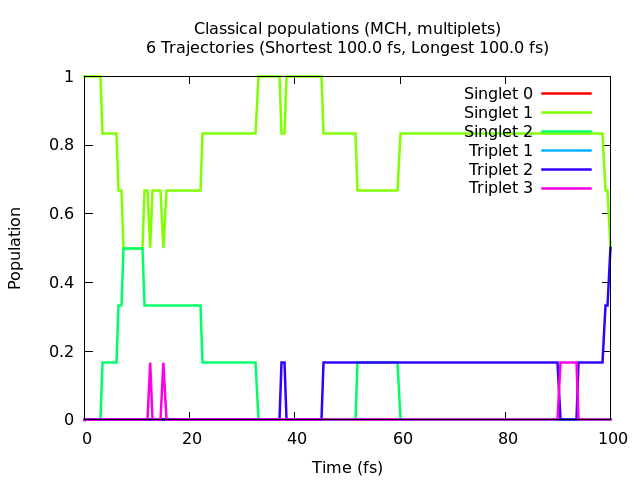
\includegraphics[width=0.8\textwidth]{figures/pop_class.png}
  \caption{Classical populations for an ensemble of 6 trajectories.}
  \label{fig:pop_class}
\end{figure}
\begin{figure}[ptb]
  \centering
  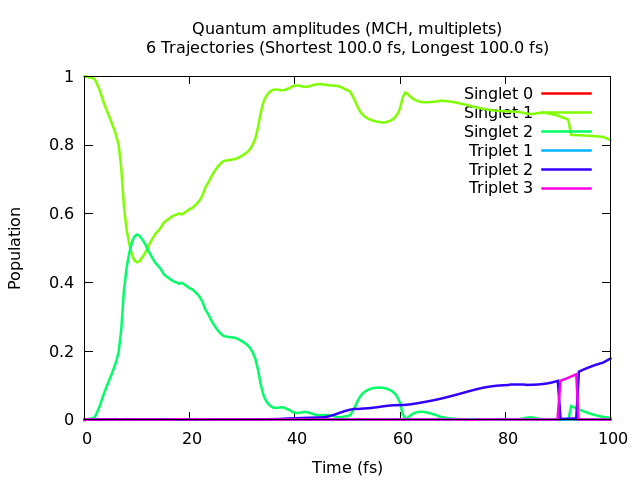
\includegraphics[width=0.8\textwidth]{figures/pop_quant.png}
  \caption{Quantum populations for an ensemble of 6 trajectories.}
  \label{fig:pop_quant}
\end{figure}
\begin{figure}[ptb]
  \centering
  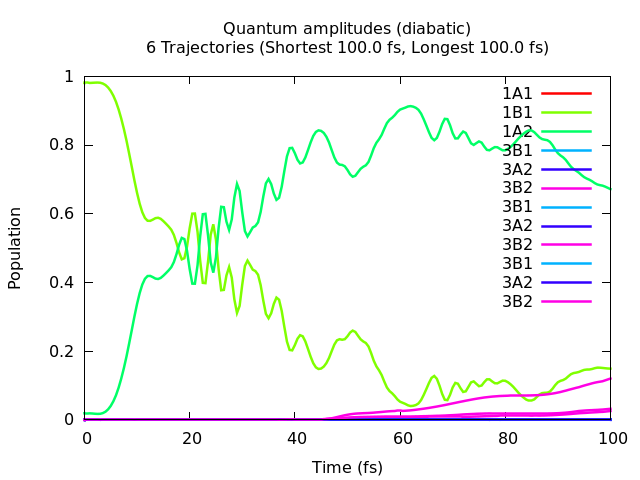
\includegraphics[width=0.8\textwidth]{figures/pop_diab.png}
  \caption{Populations of the diabatic states for an ensemble of 6 trajectories.}
  \label{fig:pop_diab}
\end{figure}


% ======================================================================================================

\clearpage
\subsection{Ensemble Populations Flow}
\refermanual{m-sec:transition.py}

In figure~\ref{fig:pop_class} it can be seen that, generally, population flows between the $S_1$ and $S_2$ and to the $T_2$.
In order to quantify this population flow, one can use \ttt{transition.py}.
This script counts the number of hops in all trajectories.

\begin{Verbatim}[commandchars=\\\{\}]
user@host> \textbf{\textcolor{red}{$SHARC/transition.py}}
\end{Verbatim}

\begin{oframed}
\footnotesize\begin{Verbatim}[commandchars=\\\{\}]
  ================================================================================
||                                                                                ||
||                   Counting hopping events from SHARC dynamics                  ||
||                                                                                ||
||                              Author: Sebastian Mai                             ||
||                                                                                ||
||                                   Version:2.1                                  ||
||                                    01.09.19                                    ||
||                                                                                ||
  ================================================================================

This script reads output.lis files files and counts all hopping events
to produce a matrix with the transition counts.
  
--------------------Paths to trajectories-------------------

Please enter the paths to all directories containing the "TRAJ_0XXXX" directories.
E.g. S_2 and S_3. 
Please enter one path at a time, and type "end" to finish the list.
Path:  [end] (autocomplete enabled) \textbf{\textcolor{red}{Singlet_1/}}
['TRAJ_00002', 'TRAJ_00003', 'TRAJ_00004', 'TRAJ_00005', 'TRAJ_00007', 'TRAJ_00010']
Found 6 subdirectories in total.

Path:  [end] (autocomplete enabled) \textbf{\textcolor{red}{<ENTER>}}

Total number of subdirectories: 6

------------------------Analyze Mode------------------------

This script finds the transition matrix:
1        In MCH basis                                                    from output.lis
2        In MCH basis (ignoring hops within one multiplet)               from output.lis

This script can also print the transition matrix for each timestep:
3        In MCH basis                                                    from output.lis
4        In MCH basis (ignoring hops within one multiplet)               from output.lis
5        In MCH basis [cumulative]                                       from output.lis
6        In MCH basis [cumulative] (ignoring hops within one multiplet)  from output.lis

Analyze mode: \textbf{\textcolor{red}{2}}

----------------------Number of states----------------------

Please enter the number of states as a list of integers
e.g. 3 0 3 for three singlets, zero doublets and three triplets.
Number of states: [3 0 3] \textbf{\textcolor{red}{<ENTER>}}

-----------------------Simulation time----------------------

Up to which simulation time should the analysis be performed?
Simulation time (in fs):  [1000.0] \textbf{\textcolor{red}{100}}


#########################Full input#########################

paths                      ['Singlet_1/']
run_extractor              False
states                     [3, 0, 3]
mode                       2
maxtime                    100.0
nstates                    6
nmstates                   12

Do you want to do the specified analysis? [True] 

Checking the directories...
Singlet_1//TRAJ_00002         OK
Singlet_1//TRAJ_00003         OK
Singlet_1//TRAJ_00004         OK
Singlet_1//TRAJ_00005         OK
Singlet_1//TRAJ_00007         OK
Singlet_1//TRAJ_00010         OK
Number of trajectories: 6
Number of steps: 201

***************************Results**************************
Full transition matrix:
        |      S0      S1      S2      T1      T2      T3
--------+------------------------------------------------
  S0    |       0       0       0       0       0       0
  S1    |       0     960       4       0       1       2
  S2    |       0       4     111       0       0       0
  T1    |       0       0       0       0       0       0
  T2    |       0       4       0       0     104       1
  T3    |       0       2       0       0       1       6

Sum transition matrix:
        |      S0      S1      S2      T1      T2      T3
--------+------------------------------------------------
  S0    |       0       0       0       0       0       0
  S1    |       0     960       8       0       5       4
  S2    |       0       0     111       0       0       0
  T1    |       0       0       0       0       0       0
  T2    |       0       0       0       0     104       2
  T3    |       0       0       0       0       0       6

Difference transition matrix:
        |      S0      S1      S2      T1      T2      T3     Sum
--------+--------------------------------------------------------
  S0    |       0       0       0       0       0       0       0
  S1    |       0       0       0       0      -3       0      -3
  S2    |       0       0       0       0       0       0       0
  T1    |       0       0       0       0       0       0       0
  T2    |       0       3       0       0       0       0       3
  T3    |       0       0       0       0       0       0       0
  Sum   |       0       3       0       0      -3       0       0
\end{Verbatim}
\end{oframed}

\normalsize

The most important matrix in the output is the difference transition matrix, which shows the ``net'' hops.
In our example, it shows that there were 3 net hops from the $S_1$ to the $T_2$.
Hence, the population flow in the ensemble is clearly $S_1\rightarrow T_2$.











% ======================================================================================================


\clearpage
\subsection{Fitting Ensemble Populations including Error Estimation}
\refermanual{m-sec:make_fitscript.py}
\refermanual{m-met:globalfit}
\refermanual{m-sec:bootstrap.py}
\refermanual{m-met:bootstrapping}

In order to facilitate comparison to experiments it is useful to obtain a time constant for the relaxation processes.
\sharc\ allows fitting population data to combinations of unimolecular reactions, using \ttt{make\_fit.py}.
Here, we will fit the population data to the kinetic model $S\rightarrow T$, which was the result of the population flow analysis.

Besides simply performing the fit, we will also obtain error estimates of the fitted time constants with the same script using the bootstrapping method.
In this method, based on the original ensemble (of 6 trajectories), ``resample'' ensembles are generated by randomly drawing \emph{with replacement} trajectories from the original ensemble (here, drawing 6 random trajectories).
Each resample is then fitted in exactly the same way as the original ensemble, and after many resamples a distribution of possible fitting parameters is obtained.
From this distribution, one can then find error measures for the fitting parameters.

In order to start the script, run:
\begin{Verbatim}[commandchars=\\\{\}]
user@host> \textbf{\textcolor{red}{$SHARC/make_fit.py}}
\end{Verbatim}


\begin{oframed}
\footnotesize\begin{Verbatim}[commandchars=\\\{\}]
  ================================================================================
||                                                                                ||
||                      Direct fitting for SHARC populations                      ||
||                                                                                ||
||                              Author: Sebastian Mai                             ||
||                                                                                ||
||                                   Version:2.1                                  ||
||                                    01.09.19                                    ||
||                                                                                ||
  ================================================================================


############################################################
#######################Kinetics Model#######################
############################################################


------------------------Model Species-----------------------

First, please specify the set of species used in your model kinetics.

Possible input:
+ <label> <label> ...   Adds one or several species to the set
- <label> <label> ...   Removes one or several species from the set
show                    Show the currently defined set of species
end                     Finish species input

Each label must be unique. Enter the labels without quotes.

Input: [end] \textbf{\textcolor{red}{+ s t }}     \textcolor{blue}{# multiple labels can be added}
  Species 's' added!
  Species 't' added!
Input: [end] \textbf{\textcolor{red}{<ENTER>}}

Final species set:  ['s', 't']

-----------------Model Elementary Reactions-----------------

Second, please specify the set of elementary reactions in your model kinetics.

Possible input:
+ <species1> <species2> <rate_label>  Add a reaction from species1 to species2 with labelled rate constant
- <rate_label>                        Remove the reaction with the given rate constant
show                                  Show the currently defined set of reactions (as adjacency matrix)
end                                   Finish reaction input

Each rate label must be unique.

Input: [end] \textbf{\textcolor{red}{+ s t k}}    \textcolor{blue}{# one reaction at a time}
  Reaction from 's' to 't' with rate label 'k' added!

Input: [end] \textbf{\textcolor{red}{<ENTER>}}

Final reaction network:
     |   s    t 
-----+----------
   s |   .    k 
   t |   .    . 

(Initial species: rows; Final species: columns)

------------------Model Initial Conditions------------------

Third, please specify species with non-zero initial populations.

Possible input:
+ <species>       Declare species to have non-zero initial population
- <species>       Remove species from the set of non-zero initial populations
show              Show the currently defined non-zero initial populations
end               Finish initial condition input

Input: [end] \textbf{\textcolor{red}{+ s}}         \textcolor{blue}{# initial population is in S1}
  Species 's' added!
Input: [end] \textbf{\textcolor{red}{<ENTER>}}

Final initial species set:  ['s']

############################################################
####################### Fitting Data #######################
############################################################


-----------------------Operation mode-----------------------

This script can work with the following output:
* pop.out (file from populations.py)
* bootstrap_data/ (directory from populations.py)
Using only the pop.out allows fitting and obtaining time constants.
Using the bootstrap data instead additionally allows for realistic error estimates.

Do you want to use bootstrap data? [False] \textbf{\textcolor{red}{yes}}
How many bootstrap samples? [100] \textbf{\textcolor{red}{<ENTER>}}


--------------------Population data file--------------------

Please specify the path to the bootstrap data directory (as generated by populations.py).

Bootstrap data directory: [bootstrap_data/] (autocomplete enabled) \textbf{\textcolor{red}{<ENTER>}}
  Detected maximal time of   100.0 fs and 7 columns (time plus 6 data columns).

Do you want to write fitting curves for all bootstrap cycles? [False] \textbf{\textcolor{red}{<ENTER>}}

------------Population-to-Species Mapping for Fit-----------

Please specify which model species should be fitted to which data file columns.
For example, you can fit the label 'S0' to column 2:
  S0 = 2
You can also fit the sum of two species to a column:
  T1 T2 = 5
You can also fit a species to the sum of several columns:
  T_all = 5 6 7
You can even fit a sum of species to a sum of columns:
  T1 T2 = 5 6 7

On the right side, "~" can be used to indicate ranges:
  T1 T2 = 5~9

Possible input:
<species1> <species2> ... = <columns1> <column2> ...            Set one mapping
show                                                            Show mapping
end                                                             Finish mapping input
reset                                                           Redo the mapping input

Each species label must be used at most once.
Each column number (except for '1', which denotes the time) must be used at most once.

Set of species:        ['s', 't']
Set of column numbers: [2, 3, 4, 5, 6, 7]
Input: [end] \textbf{\textcolor{red}{s = 2 3 4}}       \textcolor{blue}{# fit s to sum of columns 2, 3, 4 data}
Input: [end] \textbf{\textcolor{red}{t = 5 6 7}}       \textcolor{blue}{# fit t to sum of columns 5, 6, 7 data}
Input: [end] \textbf{\textcolor{red}{<ENTER>}}
Final mappings:
     s  =  2  3  4 
     t  =  5  6  7 


############################################################
##################### Fitting procedure ####################
############################################################


-------------Initial guesses------------

Please check the initial guesses for the parameters

Possible input:
label = value     Set an initial guess (detects type automatically and computes k=1/t for rates)
show              Show the currently defined non-zero initial populations
end               Finish initial condition input

  time constant ( k            ):     100.0000 fs
  initial pop   ( s            ):       1.0000

Input: [end] \textbf{\textcolor{red}{<ENTER>}}
Final guess parameters:
  time constant ( k            ):     100.0000 fs
  initial pop   ( s            ):       1.0000



------Optimize initial populations------

Do you want to optimize the initial populations (otherwise only the rates)? [True] \textbf{\textcolor{red}{no}}


--------Constrained optimization--------

Do you want to restrict all rates/initial populations to be non-negative? [True] \textbf{\textcolor{red}{<ENTER>}}

#########################Full input#########################

bootstrap_cycles           100
bounds                     True
columns_groups             [[2, 3, 4], [5, 6, 7]]
data                       [ ... ]
do_bootstrap               True
initial                    [0]
initset                    set(['s'])
maxtime                    100.0
ncol                       7
ngroups                    2
ninitial                   1
nrates                     1
nspec                      2
ntraj                      6
opt_init                   False
p0                         [0.01]
popfile                    /user/severin/workdir/ams_sharc_tutorial2/Tutorial/traj/bootstrap_data
rank                       0
rate_matrix                [['', 'k'], ['', '']]
ratemap                    {0: 'k', 'k': 0}
rates                      [[(0, 1)]]
rateset                    set(['k'])
species_groups             [['s'], ['t']]
specmap                    {0: 's', 1: 't', 's': 0, 't': 1}
summation                  [[0], [1]]
write_bootstrap_fits       False
y0                         [1.0]


Do you want to continue? [True] \textbf{\textcolor{red}{<ENTER>}}


########################## Fitting #########################


-------------- Iterations --------------

   Iteration     Total nfev        Cost      Cost reduction    Step norm     Optimality   
       0              1         2.4594e+01                                    3.98e+01    
       1              2         5.1715e+00      1.94e+01       5.53e-03       1.18e+01    
       2              3         9.9950e-01      4.17e+00       2.07e-03       3.06e+00    
       3              4         2.3208e-01      7.67e-01       8.74e-04       6.98e-01    
       4              5         1.3841e-01      9.37e-02       3.37e-04       1.13e-01    
       5              6         1.3440e-01      4.01e-03       7.99e-05       5.88e-03    
       6              7         1.3439e-01      1.23e-05       4.69e-06       2.79e-02    
       7              8         1.3439e-01      3.46e-10       2.49e-08       2.90e-07    
`ftol` termination condition is satisfied.
Function evaluations 8, initial cost 2.4594e+01, final cost 1.3439e-01, first-order optimality 2.90e-07.


----------- Final parameters -----------

time constant ( k            ):     900.2333 fs +/-      19.8598 fs (   2.21 %)
initial pop   ( s            ):       1.0000

These time constants include errors that assume that the population data
is free of uncertainty. Bootstrapping analysis is following now.

Raw data and fitted functions written to "fit_results.txt".

GNUPLOT script written to "fit_results.gp".

####################### Bootstrapping ######################

 Cycle            k            s  Time
     1   11095.5980       1.0000  0:00:00.135153
     2     904.4154       1.0000  0:00:00.049127
     3     906.8122       1.0000  0:00:00.048258
     4   10020.5031       1.0000  0:00:00.142841
     5    9967.1913       1.0000  0:00:00.141507
     \vdots       \vdots       \vdots          \vdots
   100     901.2035       1.0000  0:00:00.047236

>>>>>>>>>>>>> Finished the bootstrapping cycles ...

--------------------------------------- Analysis for time constant "k" ---------------------------------------

    Arithmetic analysis:             4503.1412 +/-    5172.8352
                                            ( +/-     114.87 %)

    Geometric analysis:              1879.7712  +     5475.4875  -     1399.3612
                                            (  +      291.28 %  -       74.44 %)

    Minimum and maximum:              298.6696      and         13663.1062

    Histogram:
    ==========
                                   #                              | 45
                                   #                              | 41
                                   #                              | 37
                                   #                 #            | 33
                                   #                 #            | 30
                                   #                 #            | 26
                                   #                 #            | 22
                                   #                 #            | 18
                             #     #                 #            | 15
                             #     #                 #            | 11
                             #     #                 #            | 7
                       #     #     #                 #            | 3
        |     |     |     |     |     |     |     |     |     |  
    31.38 71.14 161.3 365.7 829.1  1879  4261  9662 21907 49669

---------------------------------- Analysis for initial population "s" ----------------------------------

    Arithmetic analysis:                1.0000 +/-       0.0000
                                            ( +/-       0.00 %)

    Geometric analysis:                 1.0000  +        0.0000  -       -0.0000
                                            (  +        0.00 %  -       -0.00 %)

    Minimum and maximum:                1.0000      and             1.0000

    Histogram:
    ==========
     #                                                            | 100
     #                                                            | 91
     #                                                            | 83
     #                                                            | 75
     #                                                            | 66
     #                                                            | 58
     #                                                            | 50
     #                                                            | 41
     #                                                            | 33
     #                                                            | 25
     #                                                            | 16
     #                                                            | 8
        |     |     |     |     |     |     |     |     |     |  
    1.000 1.000 1.000 1.000 1.000 1.000 1.000 1.000 1.000 1.000


----------- Final parameters -----------

time constant ( k            ):     900.2333 fs +/-    5172.8352 fs ( 574.61 %)
initial pop   ( s            ):       1.0000


Output (analysis and full fitted data) written to "fit_bootstrap.txt".
\end{Verbatim}
\end{oframed}

\normalsize

Unlike the fitting scripts used in the previous \sharc\ release, \ttt{make\_fit.py} directly carries out the kinetic model fit in one program, without calling \ttt{maxima} or \ttt{gnuplot}.
It is therefore much faster, and additionally allows fitting of models that are too complex to solve analytically with \ttt{maxima}.

The main results of the script can be found under \ttt{Final parameters}, obtained after 8 iterations.
The table presents the fitted values of all parameters.
It can be seen that the $S\rightarrow T$ time constant is 900~fs with a huge and unphysical error (negative constant is in range). 
This can be explained with the fact that the transition $S\rightarrow T$ is only completed in one trajetory during and two others at the very end of the 100~fs simulation time; the population of the triplet state has not yet reached an equilibrium.
On our limited data set with only 6 trjectories, the constant is fitted to be essentially infinite or in our case 900~fs. 
A more realistic rate constant can be found at the \ttt{Geometric analysis}. 
In any case, this result suggests that for a correct analysis of the transition $S\rightarrow T$ one has to increase the simulation time and/or ensemble size.

For visual inspection of the fit results, the script writes two new files, \ttt{fit\_results.txt} and \ttt{fit\_results.gp}.
The former is a simple text file that contains three columns.
The first column is the time axis of the global fit, i.e., the time axis of the data, but continued to accommodate all data sets to be fitted (in the present case, there are three data sets to be fitted as defined in the Population-to-species mapping).
The second column is the data and the third column is the fitted kinetic model functions.
This file can be conveniently plotted with \textsc{Gnuplot}:
\begin{Verbatim}[commandchars=\\\{\}]
user@host> \textbf{\textcolor{red}{gnuplot fit_results.gp}}
\end{Verbatim}
The result of this plot is shown in Figure~\ref{fig:model_fit}.


\paragraph{Discussion of Figure~\ref{fig:model_fit}}

From the figure, it can be seen that the $S\rightarrow T$ time constant is 900~fs.
Note that the fit is not very good, because the number of trajectories is low and its quality could be improved by increasing the ensemble size.

\paragraph{Discussion of the bootstrapping results}

Because we provided bootstrapping data to the script, after the main data fit the script automatically continues the run and performs the requested number of bootstrap cycles.
In each cycle, it will write the parameters fitted for the current cycle.
Note that if the bootstrapping iterations take too long and the results seem to be converged already, pressing \ttt{Ctrl+C} allows skipping the remaining iterations and directly leads to the final analysis.

The result of the bootstrapping procedure is presented in a summary for each fitting parameter.
Note that by default also the initial populations are treated as fitting parameters, even if they are fixed in the shown example.

The results show that the $S\rightarrow T$ relaxation process in the trajectories had a time constant of 4502$\pm$5172~fs (using the arithmetic analysis). 
The histogram of the frequency of different time constants gives for information on this (note: the buckets are not well chosen in this example, so have a glance at the bootstrapping cycles). It can be seen that the time constants can be partitioned being either below 500~fs, around 900~fs or above 10000~fs. 
The reason for this lies in the composition of the individual samples, which differs a lot due to the small ensemble size. 
If a sample contains no triplet state (quite possible at only six states in the sample), then it will never make the $S\rightarrow T$ transition and the rate constant will be infinite (here a very high value). 
The other two rate constant values are obtained from samples with at least one triplet state in them. Looking at these different sample compositions, the unphysically large error can be explained. 
Again, it can be resolved with a larger ensemble (more trajectories).

Generally, the errors get smaller as more trajectories are employed, and hence, the fitting errors are a good tool to judge whether enough trajectories were computed.
For some time constants, it might also be necessary to run the trajectories for longer time to reduce the errors.
In any case, the obtained errors tell nothing about the inherent method error---using surface hopping in combination with a given quantum chemistry method.
It is not possible to quantify this method error with \ttt{make\_fit.py}; only through comparison with reference data or experiment can the method error be judged.


\begin{figure}[ptb]
  \centering
  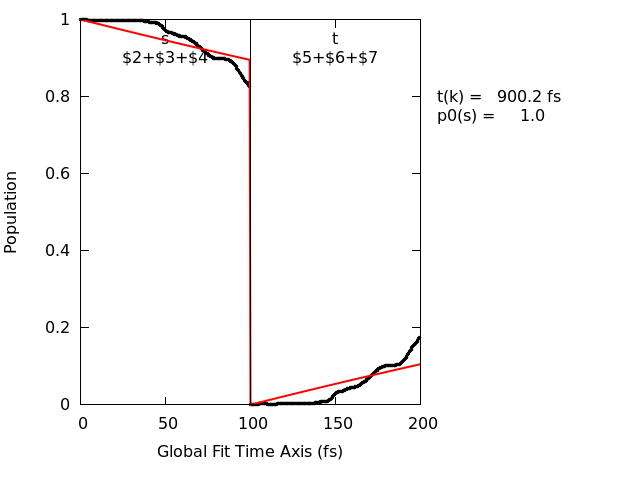
\includegraphics[width=0.8\textwidth]{figures/fit.png}
  \caption{Kinetic model fit of the classical populations.}
  \label{fig:model_fit}
\end{figure}











% ======================================================================================================

\clearpage
\subsection{Hopping Geometries}
\refermanual{m-sec:crossing.py}

Another aspect one might be interested in are certain critical geometries from the trajectories.
\ttt{crossing.py} is a script that collects those geometries from all trajectories where a surface hop between two specified states occurred.
Its usage is comparable to \ttt{populations.py}.
\begin{Verbatim}[commandchars=\\\{\}]
user@host> \textbf{\textcolor{red}{$SHARC/crossing.py}}
\end{Verbatim}

\begin{oframed}
\footnotesize\begin{Verbatim}[commandchars=\\\{\}]
  ================================================================================
||                                                                                ||
||                 Reading hopping geometries from SHARC dynamics                 ||
||                                                                                ||
||                              Author: Sebastian Mai                             ||
||                                                                                ||
||                                   Version:2.1                                  ||
||                                    01.09.19                                    ||
||                                                                                ||
  ================================================================================


This script reads output.lis files and output.xyz files to produce a list of
all geometries where certain surface hops (or other events) occured.

--------------------Paths to trajectories-------------------

Please enter the paths to all directories containing the "TRAJ_0XXXX" directories.
E.g. S_2 and S_3.
Please enter one path at a time, and type "end" to finish the list.
Path:  [end] (autocomplete enabled) \textbf{\textcolor{red}{Singlet_1/}}
['TRAJ_00005', 'TRAJ_00004', 'TRAJ_00008', 'plot.gp', 'TRAJ_00009', 'TRAJ_00002', 
'TRAJ_00006', 'TRAJ_00010', 'TRAJ_00007', 'TRAJ_00003']
Found 6 subdirectories in total.

Path:  [end] (autocomplete enabled) \textbf{\textcolor{red}{<ENTER>}}

Total number of subdirectories: 9

------------------------Analyze Mode------------------------

This script can find geometries where:
1        A change of MCH state occured (ignoring hops within one multiplet)

Analyze mode: \textbf{\textcolor{red}{1}}

----------------------Number of states----------------------

Please enter the number of states as a list of integers
e.g. 3 0 3 for three singlets, zero doublets and three triplets.
Number of states: [3 0 3] \textbf{\textcolor{red}{<ENTER>}}


---------------States involved in surface hop---------------

In this analysis mode, all geometries are fetched where a trajectory switches from a given MCH state
to another given MCH state.

Please enter the old MCH state involved as "mult state", e.g., "1 1" for S0, "1 2" for S1, or "3 1" for T1:
State 1: \textbf{\textcolor{red}{1  2}}      \textcolor{blue}{# Only hops from S1}

Please enter the new MCH state involved (mult state):
State 2: \textbf{\textcolor{red}{3  2}}      \textcolor{blue}{# to T2}

Direction:
1       Forwards      \textcolor{blue}{# Only S1 -> T2}
2       Backwards     \textcolor{blue}{# Only T2 -> S1}
3       Two-way       \textcolor{blue}{# Both S1 -> T2 and T2 -> S1}

Direction mode: [3] \textbf{\textcolor{red}{1}}

#########################Full input#########################

paths                      ['Singlet_1/']
tostates                   [[3, 2]]
run_extractor              False
states                     [3, 0, 3]
mode                       1
dirmode                    1
nstates                    6
fromstates                 [[1, 2]]
nmstates                   12

Do you want to do the specified analysis? [True] \textbf{\textcolor{red}{<ENTER>}}

Checking the directories...
Singlet_1//TRAJ_00002         OK
Singlet_1//TRAJ_00003         OK
Singlet_1//TRAJ_00004         OK
Singlet_1//TRAJ_00005         OK
Singlet_1//TRAJ_00007         OK
Singlet_1//TRAJ_00010         OK
Number of trajectories: 6

Writing to crossing.xyz ...
\end{Verbatim}
\end{oframed}

\normalsize
The script writes a files called \ttt{crossing.xyz}, which contains all geometries (6 geometries in this example) where a hop from the $S_1$ to the $T_2$ occurred.
This file can in turn be analyzed with \ttt{geo.py} in order to calculate internal coordinates (e.g., to find whether a bond or angle controls access to the $S_1/T_2$ crossing seam, or how many different pathways allow this transition). 

% ======================================================================================================

\clearpage
\subsection{Optimizing from Hopping Geometries}
\refermanual{m-sec:Orca_External}
\refermanual{m-met:orcaopt}

The output of \ttt{crossing.py} can also be used to optimize minimum-energy crossing points and conical intersections (e.g., to find how many independent crossing seam regions, i.e., reaction pathways, are involved).
In \sharc, this optimization can be automatically setup if \textsc{Orca} is installed (\textsc{Orca} is needed to perform the actual optimization of the nuclei, whereas \sharc\ provides the necessary energies and gradients).

The setup of the optimizations can be started with 
\begin{Verbatim}[commandchars=\\\{\}]
user@host> \textbf{\textcolor{red}{$SHARC/setup_orca_opt.py}}
\end{Verbatim}

\begin{oframed}
\footnotesize\begin{Verbatim}[commandchars=\\\{\}]
  ================================================================================
||                                                                                ||
||                     Setup optimizations with ORCA and SHARC                    ||
||                                                                                ||
||                      Author: Moritz Heindl, Sebastian Mai                      ||
||                                                                                ||
||                                   Version:2.1                                  ||
||                                    01.09.19                                    ||
||                                                                                ||
  ================================================================================

This script automatizes the setup of the input files ORCA+SHARC optimizations. 
  
------------------------Path to ORCA------------------------

Please specify path to ORCA directory (SHELL variables and ~ can be used, 
will be expanded when interface is started).

Path to ORCA: [$ORCADIR/] (autocomplete enabled) \textbf{\textcolor{red}{<ENTER>}}

-----------Choose the quantum chemistry interface-----------

Please specify the quantum chemistry interface (enter any of the following numbers):
1       MOLPRO (only CASSCF)
2       COLUMBUS (CASSCF, RASSCF and MRCISD), using SEWARD integrals
3       Analytical PESs
4       MOLCAS (CASSCF, CASPT2, MS-CASPT2)
5       AMS (DFT, TD-DFT)
6       TURBOMOLE (ricc2 with CC2 and ADC(2))
7       LVC Hamiltonian
8       GAUSSIAN (DFT, TD-DFT)

Interface number: \textbf{\textcolor{red}{5}}
The used interface will be: AMS (DFT, TD-DFT)

--------------------------Geometry--------------------------

Please specify the geometry file (xyz format, Angstroms):
Geometry filename: [geom.xyz] (autocomplete enabled) \textbf{\textcolor{red}{crossing.xyz}}
Number of geometries: 9

----------------------Number of states----------------------


Please enter the number of states as a list of integers
e.g. 3 0 3 for three singlets, zero doublets and three triplets.
Number of states: \textbf{\textcolor{red}{3  0  3}}

Number of states: [3, 0, 3]
Total number of states: 12

\{1: [1, 1, 0.0],
 2: [1, 2, 0.0],
 3: [1, 3, 0.0],
 4: [3, 1, -1.0],
 5: [3, 2, -1.0],
 6: [3, 3, -1.0],
 7: [3, 1, 0.0],
 8: [3, 2, 0.0],
 9: [3, 3, 0.0],
 10: [3, 1, 1.0],
 11: [3, 2, 1.0],
 12: [3, 3, 1.0]\}

---------------------States to optimize---------------------

Do you want to optimize a minimum? (no=optimize crossing): [True] \textbf{\textcolor{red}{no}}

Please specify the first state involved in the optimization
e.g. 3 2 for the second triplet state.
State: [1 2] \textbf{\textcolor{red}{<ENTER>}}

Please specify the second state involved in the optimization
e.g. 3 2 for the second triplet state.
Root: [3 2] \textbf{\textcolor{red}{<ENTER>}}
Multiplicities of both states different, optimizing a minimum crossing point.

Please enter the values for the maximum allowed displacement per timestep 
(choose smaller value if starting from a good guess and for large sigma or small alpha).
Maximum allowed step:  [0.3] \textbf{\textcolor{red}{<ENTER>}} 


  ================================================================================
||                              AMS Interface setup                               ||
  ================================================================================


------------------------Path to AMS-------------------------
Setup from amsbashrc.sh file? [True] \textbf{\textcolor{red}{<ENTER>}}

Please specify path to the amsbashrc.sh file (SHELL variables and ~ can be used, will be expanded when 
interface is started).

Path to amsbashrc.sh file: [$AMSHOME/amsbashrc.sh] \textbf{\textcolor{red}{<ENTER>}}
Will use amsbashrc= /usr/license/adf/ams2020.102/amsbashrc.sh

----------------------Scratch directory---------------------

Please specify an appropriate scratch directory. This will be used to temporally 
store the integrals. The scratch directory will be deleted after the calculation. 
Remember that this script cannot check whether the path is valid, since you may 
run the calculations on a different machine. The path will not be expanded by this script.
Path to scratch directory: (autocomplete enabled) \textbf{\textcolor{red}{$TMPDIR}}

------------------AMS input template file-------------------

Please specify the path to the AMS-ADF.template file. This file must contain the following keywords:

basis <basis>
functional <type> <name>
charge <x> [ <x2> [ <x3> ...] ]

The AMS interface will generate the appropriate AMS input automatically.

Template filename: (autocomplete enabled) \textbf{\textcolor{red}{../AMS-ADF.template}}

-----------------Initial restart: MO Guess------------------

Please specify the path to an rkf file containing suitable starting MOs for the AMS calculation. Please 
note that this script cannot check whether the wavefunction file and the Input template are consistent!

Do you have a restart file? [True] \textbf{\textcolor{red}{no}}

WARNING: Remember that the calculations may take longer without an initial guess for the MOs.
--------------------AMS Ressource usage---------------------

Please specify the number of CPUs to be used by EACH calculation.

Number of CPUs: \textbf{\textcolor{red}{1}}
-------------Wave function analysis by TheoDORE-------------


  ================================================================================
||                                 Run mode setup                                 ||
  ================================================================================


-------------------------Run script-------------------------


Where do you want to perform the calculations? Note that this script cannot check whether the path is valid.
Run directory? (autocomplete enabled) \textbf{\textcolor{red}{orca_opt/}}



#########################Full input#########################

orca                       $ORCADIR/
interface                  5
geom_location              crossing.xyz
ngeom                      4.0
natom                      3
states                     [3, 0, 3]
nstates                    12
statemap                   \{1: [1, 1, 0.0], 
                           2: [1, 2, 0.0], 
                           3: [1, 3, 0.0], 
                           4: [3, 1, -1.0], 
                           5: [3, 2, -1.0], 
                           6: [3, 3, -1.0], 
                           7: [3, 1, 0.0], 
                           8: [3, 2, 0.0], 
                           9: [3, 3, 0.0], 
                           10: [3, 1, 1.0], 
                           11: [3, 2, 1.0], 
                           12: [3, 3, 1.0]\}
maxmult                    3
opttype                    cross
cas.root1                  2
cas.root2                  5
calc_ci                    False
needed                     []
maxstep                    0.3
cwd                        /user/severin/workdir/ams_sharc_tutorial2/Tutorial/traj
amsbashrc                  /usr/license/adf/ams2020.102/amsbashrc.sh
ams                        $AMSHOME
scmlicense                 $SCMLICENSE
scratchdir                 $TMPDIR
AMS-ADF.template               ../AMS-ADF.template
ams.guess                  \{\}
ams.ncpu                   1
ams.scaling                0.9
theodore                   False
here                       False
copydir                    orca_opt

Do you want to setup the specified calculations? [True] \textbf{\textcolor{red}{<ENTER>}}

  ================================================================================
||                             Setting up directory...                            ||
  ================================================================================
\end{Verbatim}
\end{oframed}

\normalsize
The script will create 6 subdirectories in the given setup directory, \ttt{orca\_opt/}.
Each of these 6 directories will contain the input files for an optimization using \textsc{Orca}'s external optimizer feature, where the energies and gradients will be provided by \ttt{\$SHARC/orca\_External} (this is done automatically), which itself calls the \textsc{AMS} interface to do the computations.

In order to run one of these optimizations, execute:
\begin{Verbatim}[commandchars=\\\{\}]
user@host> \textbf{\textcolor{red}{cd orca_opt/geom_4/}}
user@host> \textbf{\textcolor{red}{sh run_EXTORCA.sh&}}
\end{Verbatim}
The progress of the optimization can be followed in \ttt{orca.log}. In this file, note the lines following \ttt{EXTERNAL SHARC JOB}, which are written by \sharc\ and show the computed energies and gradients.
Close to a box labeled \ttt{Geometry convergence}, \textsc{Orca} reports the convergence status of the optimization.
After 11~cycles, the optimization should converge; the energies of $S_2$ and $T_2$ at convergence should be $-0.4803104749$ and $-0.4803034819$~Hartree.
This is a very good result, as the energy gap is only 0.000007~eV; if the gap was much larger, then the optimization should be repeated (starting from the last step) with adjusted optimization parameters (see the manual).




% ======================================================================================================

\clearpage
\subsection{Essential Dynamics Analysis}
\refermanual{m-sec:trajana_essdyn.py}
\refermanual{m-met:essdyn}

Another possibility to investigate nuclear motion in the trajectories is given by the essential dynamics analysis.
This analysis simply takes all trajectories and identifies collective motion, which can be useful to find reaction paths or to construct reduced-dimensionality models.

The interactive script can be started with 
\begin{Verbatim}[commandchars=\\\{\}]
user@host> \textbf{\textcolor{red}{$SHARC/trajana_essdyn.py}}
\end{Verbatim}

\begin{oframed}
\footnotesize\begin{Verbatim}[commandchars=\\\{\}]
  ================================================================================
||                                                                                ||
||                 Essential dynamics analysis for SHARC dynamics                 ||
||                                                                                ||
||                      Author: Felix Plasser, Andrew Atkins                      ||
||                                                                                ||
||                                   Version:2.1                                  ||
||                                    01.09.19                                    ||
||                                                                                ||
  ================================================================================


This script reads output.xyz files and calculates the essential dynamics 
(i.e., Shows you which are the most important motions).
  
--------------------Paths to trajectories-------------------

Please enter the paths to all directories containing the "TRAJ_0XXXX" directories.
E.g. Sing_2/ and Sing_3/. 
Please enter one path at a time, and type "end" to finish the list.
Path:  [end] (autocomplete enabled) \textbf{\textcolor{red}{Singlet_1/}}
['TRAJ_00002', 'TRAJ_00003', 'TRAJ_00004', 'TRAJ_00005', 'TRAJ_00007', 'TRAJ_00010']
Found 6 subdirectories in total.

Path:  [end] (autocomplete enabled) \textbf{\textcolor{red}{<ENTER>}}

Total number of subdirectories: 6

-----------------Path to reference structure----------------

Please enter the path to the equilibrium structure of your system (in the same
atomic order as that given in the dynamics output)

Path:  [ref.xyz] (autocomplete enabled) \textbf{\textcolor{red}{../AMS.freq.molden}}

Please give the type of coordinate file [molden] (autocomplete enabled) \textbf{\textcolor{red}{<ENTER>}}

Do you wish to use mass weighted coordinates? [True] \textbf{\textcolor{red}{<ENTER>}}

---------Number of total steps in your trajectories---------

Number of time steps:  [201] \textbf{\textcolor{red}{<ENTER>}}

--------------The time step of your calculation-------------

Length of time step:  [0.5] \textbf{\textcolor{red}{<ENTER>}}

------------------Time steps to be analysed-----------------

Please enter the time step intervals for which the statistical analysis should be carried out. 

Time step interval:  [0 200] \textbf{\textcolor{red}{0  40}}

Do you want to add another time interval for analysis? [False] \textbf{\textcolor{red}{<ENTER>}}

----------------------Results directory---------------------
Please give the name of the subdirectory to be used for the results (use to save similar analysis
in separate subdirectories).
Name for subdirectory? [essdyn] (autocomplete enabled) \textbf{\textcolor{red}{<ENTER>}}

Preparing essential dynamics analysis ...
Checking the directories...
Singlet_1//TRAJ_00002         OK
Singlet_1//TRAJ_00003         OK
Singlet_1//TRAJ_00004         OK
Singlet_1//TRAJ_00005         OK
Singlet_1//TRAJ_00007         OK
Singlet_1//TRAJ_00010         OK
Number of trajectories: 6
Reading trajectory Singlet_1//TRAJ_00002/output.xyz ...
Reading trajectory Singlet_1//TRAJ_00003/output.xyz ...
Reading trajectory Singlet_1//TRAJ_00004/output.xyz ...
Reading trajectory Singlet_1//TRAJ_00005/output.xyz ...
Reading trajectory Singlet_1//TRAJ_00007/output.xyz ...
Reading trajectory Singlet_1//TRAJ_00010/output.xyz ...
Processing data ...
\end{Verbatim}
\end{oframed}

\normalsize
The output of this script is a directory \ttt{ESS\_DYN/essdyn/}, which contains two subdirectories with the results of the total covariance analysis (\ttt{total\_cov/}, giving the most active modes) and of the analysis of the average trajectory (\ttt{cross\_av/}, giving the most active \emph{coherent} modes).
Each directory will contain one output file for the chosen time step interval (steps 0 to 40) called \ttt{0-40.molden}.
The content of the file is similar to that of a frequency calculation, containing the average geometry of the molecule in the interval and the essential dynamics modes.
The ``frequency'' entries for the essential modes give the total activity of the mode, with larger values indicating more active modes.
In order to find the most important motions of the molecule, visualize the essential modes with the largest ``frequencies''.
A vector representation of the most important mode in \ttt{ESS\_DYN/essdyn/cross\_av/0-40.molden} is shown in Figure~\ref{fig:essdyn}.

\begin{figure}[pb]
  \centering
  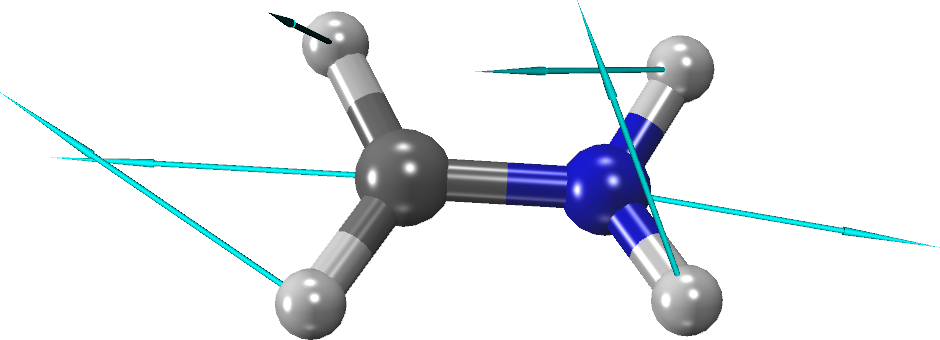
\includegraphics[width=0.7\textwidth]{figures/essdyn.png}
  \caption{Vector representation of the most active essential mode.}
  \label{fig:essdyn}
\end{figure}


% ======================================================================================================

\clearpage
\subsection{Normal Mode Analysis}
\refermanual{m-sec:trajana_nma.py}
\refermanual{m-met:nma}

An alternative to the essential dynamics analysis is a normal mode analysis.
The difference is that the essential dynamics analysis automatically identifies a suitable set of modes, whereas the normal mode analysis uses a set of precomputed normal modes (e.g., normal modes of the ground state minimum).

The interactive script can be started with 
\begin{Verbatim}[commandchars=\\\{\}]
user@host> \textbf{\textcolor{red}{$SHARC/trajana_nma.py}}
\end{Verbatim}

\begin{oframed}
\footnotesize\begin{Verbatim}[commandchars=\\\{\}]
  ================================================================================
||                                                                                ||
||                     Normal-mode analysis for SHARC dynamics                    ||
||                                                                                ||
||                      Author: Felix Plasser, Andrew Atkins                      ||
||                                                                                ||
||                                   Version:2.1                                  ||
||                                    01.09.19                                    ||
||                                                                                ||
  ================================================================================

This script reads output.xyz files, transforms into normal modes, and performs statistical analyses 
(i.e., Shows you which are the most important motions).
  
--------------------Paths to trajectories-------------------

Please enter the paths to all directories containing the "TRAJ_0XXXX" directories.
E.g. Sing_2/ and Sing_3/. 
Please enter one path at a time, and type "end" to finish the list.
Path:  [end] (autocomplete enabled) \textbf{\textcolor{red}{Singlet_1/}}
['TRAJ_00002', 'TRAJ_00003', 'TRAJ_00004', 'TRAJ_00005', 'TRAJ_00007', 'TRAJ_00010']
Found 6 subdirectories in total.

Path:  [end] (autocomplete enabled) \textbf{\textcolor{red}{<ENTER>}}

Total number of subdirectories: 6

------------------Path to normal mode file------------------

Please enter the path to the Molden normal mode file for your molecule. 
The contained geometry will be used as reference geometry.
(Atomic order must be the same as in the trajectories!)

Path:  (autocomplete enabled) \textbf{\textcolor{red}{../AMS.freq.molden}}

Do you wish to use mass weighted normal modes? [True] \textbf{\textcolor{red}{<ENTER>}}

---------Number of total steps in your trajectories---------

Number of time steps:  [201] \textbf{\textcolor{red}{<ENTER>}}

--------------The time step of your calculation-------------

Length of time step:  [0.5] \textbf{\textcolor{red}{<ENTER>}}

\textcolor{blue}{# make sure to have matplotlib installed to see this prompt}
-------------------Automatic plot creation------------------
Do you want to automatically create plots of your data? [False] yes 

-------------Non-totally symmetric normal modes-------------

Please enter the numbers of the normal modes (numbering as in the Molden file) whose absolute 
value should be considered in the analysis. Without this setting, the average for all 
non-totally symmetric modes should be zero. Default is to not compute the absolute. 
Entering -1 ends this input section.

Non-totally symmetric normal modes: [-1] (range comprehension enabled) \textbf{\textcolor{red}{1~3}}
Non-totally symmetric normal modes: [-1] (range comprehension enabled) \textbf{\textcolor{red}{<ENTER>}}

--------------------Multiplication by -1--------------------
Please enter the numbers of normal modes whose values should be multiplied by -1 before 
statistical analysis (affects total_std.txt and cross_av_std.txt). This is only for convenience
when viewing the results. Entering -1 ends this input section.

Inverted normal modes: [-1] (range comprehension enabled) \textbf{\textcolor{red}{<ENTER>}}

------------------Time steps to be analysed-----------------

Please enter the time step intervals for which the statistical analysis should be carried out. 

Time step interval:  [0 200] \textbf{\textcolor{red}{<ENTER>}}

Do you want to add another time interval for analysis? [False] \textbf{\textcolor{red}{<ENTER>}}

----------------------Results directory---------------------
Please give the name of the subdirectory to be used for the results (use to save similar 
analysis in separate subdirectories).
Name for subdirectory? [nma] (autocomplete enabled) \textbf{\textcolor{red}{<ENTER>}}

Preparing NMA ...
Checking the directories...
Singlet_1//TRAJ_00002         OK
Singlet_1//TRAJ_00003         OK
Singlet_1//TRAJ_00004         OK
Singlet_1//TRAJ_00005         OK
Singlet_1//TRAJ_00007         OK
Singlet_1//TRAJ_00010         OK
Number of trajectories: 6
Reading trajectory Singlet_1//TRAJ_00002/output.xyz ...
Reading trajectory Singlet_1//TRAJ_00003/output.xyz ...
Reading trajectory Singlet_1//TRAJ_00004/output.xyz ...
Reading trajectory Singlet_1//TRAJ_00005/output.xyz ...
Reading trajectory Singlet_1//TRAJ_00007/output.xyz ...
Reading trajectory Singlet_1//TRAJ_00010/output.xyz ...
Processing data ...
\end{Verbatim}
\end{oframed}

\normalsize
The output of this script is a directory \ttt{NMA/nma/}, which contains four output files, \ttt{mean\_against\_time.txt} and \ttt{std\_against\_time.txt}, \ttt{total\_std.txt}, and \ttt{cross\_av\_std.txt}.
The content of the first two files is plotted in subdirectory \ttt{time\_plots/}, whereas the content of the two other files is plotted in subdirectory \ttt{bar\_graphs/}.

The file  \ttt{NMA/nma/bar\_graphs/total\_std/0-200.png} is plotted in Figure~\ref{fig:nma}.
It shows that the most active mode is mode~1, which is the symmetric bend mode, followed by modes 2 and 3, which are the asymmetric and symmetric stretch modes.

Note that \ttt{trajana\_nma.py} also produces output files in all trajectory folders.
These files contain the coordinates of the trajectory converted to normal mode coordinates (complementary to output of \ttt{geo.py}).

\begin{figure}[ptb]
  \centering
  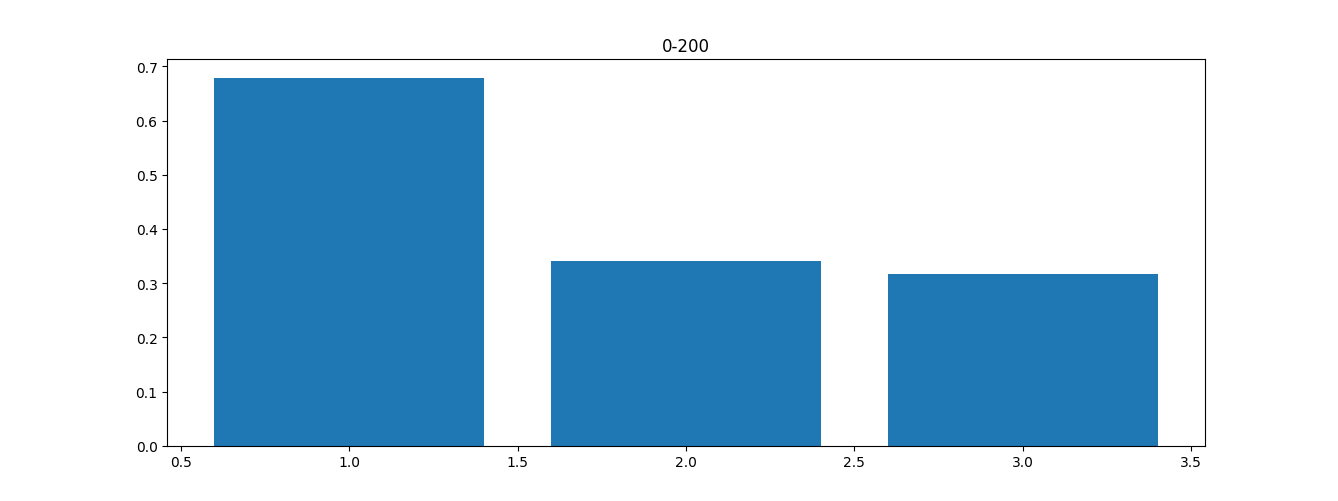
\includegraphics[width=0.7\textwidth]{figures/nma.png}
  \caption{Total activity of the normal modes of \ce{SO2}. Plotted is the relative activity in percent against the three normal modes. Mode 1 shows the highest activity with almost 70\%.}
  \label{fig:nma}
\end{figure}




% ======================================================================================================

\clearpage
\subsection{Ensemble Motion Plots}
\refermanual{m-sec:data_collector.py}

In addition to the statistical analysis of the nuclear motion (\ttt{trajana\_essdyn.py} and \ttt{trajana\_nma.py}), it is often helpful to plot some bond length, angle, internal coordinate, etc.\ for all trajectories, in what could be called ``hair figures'' or heat maps.
For such plots (and many others), \ttt{data\_collector.py} can merge the corresponding per-trajectory data into files which can then be conveniently plotted.

In the following, we will collect the time-dependent \ce{C=N} bond length from all trajectories and plot them.
The first step is to compute this bond length for each trajectory.
This can be achieved with \ttt{geo.py} and a simple Bash loop:
\begin{Verbatim}[commandchars=\\\{\}]
user@host> \textbf{\textcolor{red}{echo "r 1 2" > Geo.inp}}
user@host> \textbf{\textcolor{red}{for i in Singlet_1/TRAJ_000*}}
> \textbf{\textcolor{red}{do}}
> \textbf{\textcolor{red}{$SHARC/geo.py -t 0.5 -g $i/output.xyz < Geo.inp > $i/Geo.out;}}
> \textbf{\textcolor{red}{done}}
\end{Verbatim}
This will create a file \ttt{Geo.out} for each trajectory with the bond length between atoms 1 and 2.

Then, start the \ttt{data\_collector.py} to merge the data into a single file (note that the excluded trajectories are ignored):
\begin{Verbatim}[commandchars=\\\{\}]
user@host> \textbf{\textcolor{red}{$SHARC/data_collector.py}}
\end{Verbatim}

\begin{oframed}
\footnotesize\begin{Verbatim}[commandchars=\\\{\}]
  ================================================================================
||                                                                                ||
||                     Reading table data from SHARC dynamics                     ||
||                                                                                ||
||                              Author: Sebastian Mai                             ||
||                                                                                ||
||                                   Version:2.1                                  ||
||                                    01.09.19                                    ||
||                                                                                ||
  ================================================================================


This script collects table data from SHARC trajectories, smooths them, synchronizes them,
convolutes them, and computes averages and similar statistics.
  
--------------------Paths to trajectories-------------------

Please enter the paths to all directories containing the "TRAJ_0XXXX" directories.
E.g. Sing_2/ and Sing_3/. 
Please enter one path at a time, and type "end" to finish the list.
Path:  [end] (autocomplete enabled) \textbf{\textcolor{red}{Singlet_1/}}
['TRAJ_00002', 'TRAJ_00003', 'TRAJ_00004', 'TRAJ_00005', 'TRAJ_00007', 'TRAJ_00010']
Found 6 subdirectories in total.

Path:  [end] (autocomplete enabled) \textbf{\textcolor{red}{<ENTER>}}

Total number of subdirectories: 6

Checking the directories...
Number of trajectories: 6
Checking for common files...

List of files common to the trajectory directories:

 Index Number of appearance   Relative file path
----------------------------------------------------------
     0                    6   ./Geo.out
     1                    6   ./nma_nma.txt
     2                    6   ./nma_nma_av.txt
     3                    6   ./nma_nma_std.txt
     4                    6   ./output.lis
     5                    6   QM/AMS-ADF.resources
     6                    6   QM/AMS-ADF.template
     7                    6   output_data/coeff_MCH.out
     8                    6   output_data/coeff_class_MCH.out
     9                    6   output_data/coeff_class_diab.out
    10                    6   output_data/coeff_class_diag.out
    11                    6   output_data/coeff_diab.out
    12                    6   output_data/coeff_diag.out
    13                    6   output_data/coeff_mixed_MCH.out
    14                    6   output_data/coeff_mixed_diab.out
    15                    6   output_data/coeff_mixed_diag.out
    16                    6   output_data/energy.out
    17                    6   output_data/expec.out
    18                    6   output_data/expec_MCH.out
    19                    6   output_data/fosc.out
    20                    6   output_data/fosc_act.out
    21                    6   output_data/prob.out
    22                    6   output_data/spin.out

Please give the relative file path of the file you want to collect:
File path or index: [0] \textbf{\textcolor{red}{<ENTER>}}

------------------------Data columns------------------------

Number of columns in the file:   2

Please select the data columns for the analysis:
For T column: 
  only enter one (positive) column index. 
  If 0, the line number will be used instead.
For X column: 
  enter one or more column indices. 
  If 0, all entries of that column will be set to 1. 
  If negative, the read numbers will be multiplied by -1.
For Y column: 
  enter as many column indices as for X. 
  If 0, all entries of that column will be set to 1. 
  If negative, the read numbers will be multiplied by -1.

T column (time): [1] \textbf{\textcolor{red}{<ENTER>}}
X columns: [2] (range comprehension enabled) \textbf{\textcolor{red}{<ENTER>}}
Y columns: [0] (range comprehension enabled) \textbf{\textcolor{red}{<ENTER>}}
Selected columns:
T: 1     X: [2]    Y: [0]

---------------------Analysis procedure---------------------

Show possible workflow options? [True] \textbf{\textcolor{red}{no}}

---------------1 Smoothing--------------

Do you want to apply smoothing to the individual trajectories? [False] \textbf{\textcolor{red}{<ENTER>}}

-------------2 Synchronizing------------

Do you want to synchronize the data? [True] \textbf{\textcolor{red}{<ENTER>}}


----------3 Convoluting along X---------

Do you want to apply convolution in X direction? [False] \textbf{\textcolor{red}{yes}}

Choose one of the following convolution kernels:
1  Gaussian function
2  Lorentzian function
3  Rectangular window function
4  Log-normal function
Choose one of the functions: [1] \textbf{\textcolor{red}{<ENTER>}}
Choose width of the smoothing function (in units of the X columns): [1.0] \textbf{\textcolor{red}{0.2}}
Size of the grid along X: [25] \textbf{\textcolor{red}{50}}

Choose minimum and maximum of the grid along X:
Enter either a single number a (X grid from  xmin-a*width  to  xmax+a*width)
        or two numbers a and b (X grid from  a  to  b)
Xrange: [1.0] \textbf{\textcolor{red}{1.5}}

------------6 Sum over all Y------------

Do you want to sum up all Y values? [False] \textbf{\textcolor{red}{<ENTER>}}

-----------7 Integrate along X----------

Do you want to integrate in X direction? [False] \textbf{\textcolor{red}{<ENTER>}}

----------8 Convoluting along T---------

Do you want to apply convolution in T direction? [False] \textbf{\textcolor{red}{<ENTER>}}

----------9 Integrating along T---------

Do you want to integrate in T direction? [False] \textbf{\textcolor{red}{<ENTER>}}

-------10 Convert to Type2 dataset------

If you performed integration along X, the data might be better formatted as Type2 dataset.
Do you want to output as Type2 dataset? [False] \textbf{\textcolor{red}{<ENTER>}}


#########################Full input#########################

paths                      ['Singlet_1/']
statistics                 \{\}
allfiles                   ['Singlet_1//TRAJ_00002/./Geo.out', 'Singlet_1//TRAJ_00003/./Geo.out',
                            'Singlet_1//TRAJ_00004/./Geo.out', 'Singlet_1//TRAJ_00005/./Geo.out',
                            'Singlet_1//TRAJ_00007/./Geo.out', 'Singlet_1//TRAJ_00010/./Geo.out']
colX                       [2]
filepath                   ./Geo.out
averaging                  \{\}
colT                       1
colY                       [0]
synchronizing              True
smoothing                  \{\}
nX                         1
nY                         1
convolute_T                \{\}
ncol                       2
type3_to_type2             False
integrate_X                \{\}
sum_Y                      False
integrate_T                False
convolute_X                \{'function': <__main__.gauss instance at 0x7fc7c22bcfa0>, 
                            'npoints': 50, 
                            'xrange': [1.5]\}

Do you want to do the specified analysis? [True] 



>>>>>>>>>>>>>>>>>>>>>> Started data analysis

Collecting the data ...
  Progress: [==================================================] 100%
>>>> Writing output to file "collected_data_1_2_0.type1.txt"...

Synchronizing temporal data ...
  Progress: [==================================================] 100%
>>>> Writing output to file "collected_data_1_2_0_sy.type2.txt"...

Convoluting data (along X column) ...
  Progress: [==================================================] 100%
>>>> Writing output to file "collected_data_1_2_0_sy_cX.type3.txt"...


Finished!
\end{Verbatim}
\end{oframed}

\normalsize
This run of the script produces three output files:
\begin{itemize}
  \item \ttt{collected\_data\_1\_2\_0.type1.txt},
  \item \ttt{collected\_data\_1\_2\_0\_sy.type2.txt}, and
  \item \ttt{collected\_data\_1\_2\_0\_sy\_cX.type3.txt}.
\end{itemize}
You can plot the contained data using \textsc{Gnuplot} (do not type the line break):
\begin{Verbatim}[commandchars=\\\{\}]
gnuplot> \textbf{\textcolor{red}{p "collected_data_1_2_0_sy.type2.txt" u 1:2 w l, "" u 1:3 w l,}}
         \textbf{\textcolor{red}{"" u 1:4 w l, "" u 1:5 w l, "" u 1:6 w l, "" u 1:7 w l}}
\end{Verbatim}
or (if using \textsc{Gnuplot} 5.0 or higher):
\begin{Verbatim}[commandchars=\\\{\}]
gnuplot> \textbf{\textcolor{red}{p for [col=2:7] "collected_data_1_2_0_sy.type2.txt" u 1:col w l}}
\end{Verbatim}
For the 3D data in \ttt{collected\_data\_1\_2\_0\_sy\_cX.type3.txt}, use:
\begin{Verbatim}[commandchars=\\\{\}]
gnuplot> \textbf{\textcolor{red}{set view map}}
gnuplot> \textbf{\textcolor{red}{sp "collected_data_1_2_0_sy_cX.type3.txt" u 1:2:3 w pm3d}}
\end{Verbatim}
The results of these two plot commands are shown in Figures~\ref{fig:coll_1_2} and \ref{fig:coll_1_2_cX}.

Using \ttt{data\_collector.py}, it is also possible to compute the mean and standard deviations of the bond lengths (giving similar information as \ttt{trajana\_nma.py} was doing for the normal modes).
In order to do so, do not apply convolution in X direction, and then ask for an averaging and/or statistics analysis.


\begin{figure}[p]
  \centering
  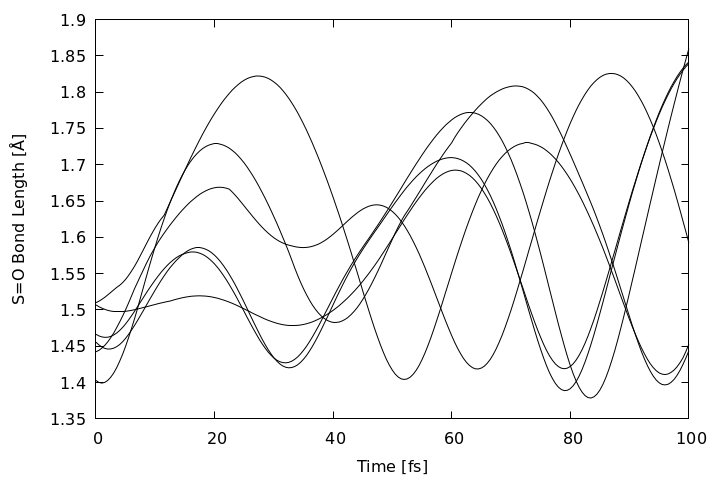
\includegraphics[width=0.7\textwidth]{figures/coll_1_2.png}
  \caption{All \ce{SO} bond lengths from the 6 trajectories.}
  \label{fig:coll_1_2}
\end{figure}

\begin{figure}[p]
  \centering
  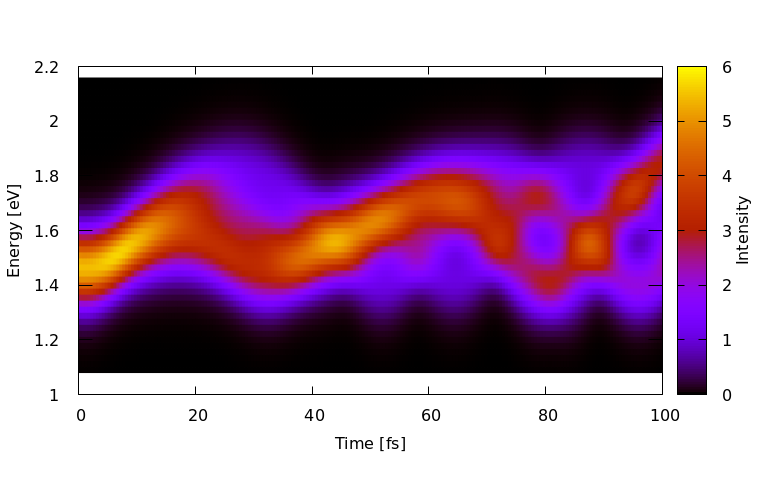
\includegraphics[width=0.7\textwidth]{figures/coll_1_2_cX.png}
  \caption{Convolution of the \ce{SO} bond lengths from the 6 trajectories.}
  \label{fig:coll_1_2_cX}
\end{figure}











% ======================================================================================================

\clearpage
\subsection{Ultrafast Time-Resolved Emission Spectrum}
\refermanual{m-sec:data_collector.py}

Using \ttt{data\_collector.py}, it is also possible to compute ultrafast time-resolve emission spectra.
Here, we will simulate the emission spectrum for \ce{SO2}.

Again, start the \ttt{data\_collector.py} to merge and post-process the data:
\begin{Verbatim}[commandchars=\\\{\}]
user@host> \textbf{\textcolor{red}{$SHARC/data_collector.py}}
\end{Verbatim}

\begin{oframed}
\footnotesize\begin{Verbatim}[commandchars=\\\{\}]
  ================================================================================
||                                                                                ||
||                     Reading table data from SHARC dynamics                     ||
||                                                                                ||
||                              Author: Sebastian Mai                             ||
||                                                                                ||
||                                   Version:2.1                                  ||
||                                    01.09.19                                    ||
||                                                                                ||
  ================================================================================


This script collects table data from SHARC trajectories, smooths them, synchronizes them,
convolutes them, and computes averages and similar statistics.
  
--------------------Paths to trajectories-------------------

Please enter the paths to all directories containing the "TRAJ_0XXXX" directories.
E.g. Sing_2/ and Sing_3/. 
Please enter one path at a time, and type "end" to finish the list.
Path:  [end] (autocomplete enabled) \textbf{\textcolor{red}{Singlet_1/}}
['TRAJ_00002', 'TRAJ_00003', 'TRAJ_00004', 'TRAJ_00005', 'TRAJ_00007', 'TRAJ_00010']
Found 6 subdirectories in total.

Path:  [end] (autocomplete enabled) \textbf{\textcolor{red}{<ENTER>}}

Total number of subdirectories: 6

Checking the directories...
Number of trajectories: 6
Checking for common files...

List of files common to the trajectory directories:

 Index Number of appearance   Relative file path
----------------------------------------------------------
     0                    7   ./Geo.out
     1                    7   ./nma_nma.txt
     2                    7   ./nma_nma_av.txt
     3                    7   ./nma_nma_std.txt
     4                    7   ./output.lis
     5                    7   output_data/coeff_MCH.out
     6                    7   output_data/coeff_diab.out
     7                    7   output_data/coeff_diag.out
     8                    7   output_data/energy.out
     9                    7   output_data/expec.out
    10                    7   output_data/expec_MCH.out
    11                    7   output_data/fosc.out
    12                    7   output_data/fosc_act.out
    13                    7   output_data/prob.out
    14                    7   output_data/spin.out

Please give the relative file path of the file you want to collect:
File path or index: [0] \textbf{\textcolor{red}{output_data/fosc_act.out}}

------------------------Data columns------------------------

Number of columns in the file:   25

Please select the data columns for the analysis:
For T column: 
  only enter one (positive) column index. 
  If 0, the line number will be used instead.
For X column: 
  enter one or more column indices. 
  If 0, all entries of that column will be set to 1. 
  If negative, the read numbers will be multiplied by -1.
For Y column: 
  enter as many column indices as for X. 
  If 0, all entries of that column will be set to 1. 
  If negative, the read numbers will be multiplied by -1.

T column (time): [1] \textbf{\textcolor{red}{<ENTER>}}
X columns: [2] (range comprehension enabled) \textbf{\textcolor{red}{2~13}}
Y columns: [0 0 0 0 0 0 0 0 0 0 0 0 0] (range comprehension enabled) \textbf{\textcolor{red}{14~25}}
Selected columns:
T: 1     X: [2, 3, 4, 5, 6, 7, 8, 9, 10, 11, 12, 13]    
         Y: [14, 15, 16, 17, 18, 19, 20, 21, 22, 23, 24, 25]

---------------------Analysis procedure---------------------

Show possible workflow options? [True] \textbf{\textcolor{red}{no}}

---------------1 Smoothing--------------

Do you want to apply smoothing to the individual trajectories? [False] \textbf{\textcolor{red}{<ENTER>}}

-------------2 Synchronizing------------

Do you want to synchronize the data? [True] \textbf{\textcolor{red}{<ENTER>}}

----------3 Convoluting along X---------

Do you want to apply convolution in X direction? [False] \textbf{\textcolor{red}{yes}}

Choose one of the following convolution kernels:
1  Gaussian function
2  Lorentzian function
3  Rectangular window function
4  Log-normal function
Choose one of the functions: [1] \textbf{\textcolor{red}{<ENTER>}}
Choose width of the smoothing function (in units of the X columns): [1.0] \textbf{\textcolor{red}{<ENTER>}}
Size of the grid along X: [25] \textbf{\textcolor{red}{50}}

Choose minimum and maximum of the grid along X:
Enter either a single number a (X grid from  xmin-a*width  to  xmax+a*width)
        or two numbers a and b (X grid from  a  to  b)
Xrange: [1.0] \textbf{\textcolor{red}{1.5}}

------------6 Sum over all Y------------

Do you want to sum up all Y values? [False] \textbf{\textcolor{red}{yes}}

-----------7 Integrate along X----------

Do you want to integrate in X direction? [False] \textbf{\textcolor{red}{<ENTER>}}

----------8 Convoluting along T---------

Do you want to apply convolution in T direction? [False] \textbf{\textcolor{red}{<ENTER>}}

----------9 Integrating along T---------

Do you want to integrate in T direction? [False] \textbf{\textcolor{red}{<ENTER>}}

-------10 Convert to Type2 dataset------

If you performed integration along X, the data might be better formatted as Type2 dataset.
Do you want to output as Type2 dataset? [False] \textbf{\textcolor{red}{<ENTER>}}


#########################Full input#########################

paths                      ['Singlet_1/']
statistics                 \{\}
allfiles                   ['Singlet_1//TRAJ_00002/output_data/fosc_act.out',
                            'Singlet_1//TRAJ_00003/output_data/fosc_act.out',
                            'Singlet_1//TRAJ_00004/output_data/fosc_act.out', 
                            'Singlet_1//TRAJ_00005/output_data/fosc_act.out', 
                            'Singlet_1//TRAJ_00007/output_data/fosc_act.out', 
                            'Singlet_1//TRAJ_00010/output_data/fosc_act.out']
colX                       [2, 3, 4, 5, 6, 7, 8, 9, 10, 11, 12, 13]
filepath                   output_data/fosc_act.out
averaging                  \{\}
colT                       1
colY                       [14, 15, 16, 17, 18, 19, 20, 21, 22, 23, 24, 25]
synchronizing              True
smoothing                  \{\}
nX                         12
nY                         12
convolute_T                \{\}
ncol                       25
type3_to_type2             False
integrate_X                \{\}
sum_Y                      True
integrate_T                False
convolute_X                \{'function': <__main__.gauss instance at 0x7fb48fc36b40>, 
                            'npoints': 50, 
                            'xrange': [1.5]\}

Do you want to do the specified analysis? [True] 



>>>>>>>>>>>>>>>>>>>>>> Started data analysis

Collecting the data ...
  Progress: [==================================================] 100%
>>>> Writing output to file "collected_data_1_2345678910111213_141516171819202122232425.type1.txt"...

Synchronizing temporal data ...
  Progress: [==================================================] 100%
>>>> Writing output to file "collected_data_1_2345678910111213_141516171819202122232425_sy.type2.txt"...

Convoluting data (along X column) ...
  Progress: [==================================================] 100%
>>>> Writing output to file "collected_data_1_2345678910111213_141516171819202122232425_sy_cX.type3.txt"...

Summing all Y values ...
  Progress: [==================================================] 100%
>>>> Writing output to file "collected_data_1_2345678910111213_141516171819202122232425_sy_cX_sY.type3.txt"
...


Finished!
\end{Verbatim}
\end{oframed}

\normalsize
The last of the four produced output files contains the total emission spectrum.
You can print it in the same way as the convoluted bond lengths in Figure~\ref{fig:coll_1_2_cX}.
The simulated spectrum is presented in Figure~\ref{fig:emission_spec}.

Using \ttt{data\_collector.py}, it is also possible to convolute the spectrum with an instrument response function, or to integrate it along the time or energy axes.

\begin{figure}[h]
  \centering
  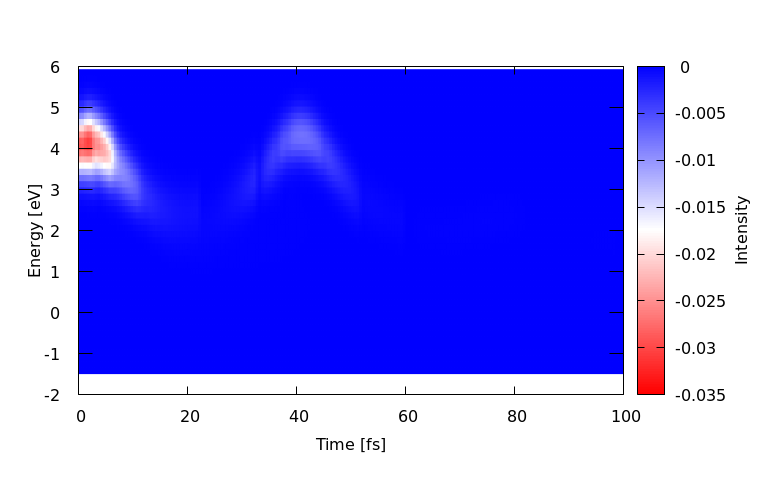
\includegraphics[width=0.9\textwidth]{figures/emission_spec.png}
  \caption{Simulated ultrafast time-resolved emission spectrum of \ce{SO2}. Ground state bleech (negative absorption) is shown in red, and excited-state absorption (positive absorption) is shown in blue.}
  \label{fig:emission_spec}
\end{figure}



% ======================================================================================================
\clearpage
\section{Setting up LVC models}
\label{sec:setup_LVC}
\refermanual{m-sec:int:lvc}
\refermanual{m-sec:setup_LVCparam.py}

Linear vibronic coupling (LVC) models are analytical model potentials that can be automatically paramatrized from a small number of quantum chemistry calculations.
Subsequently, running \sharc\ on these model potentials can be an extremely efficient way to simulate nonadiabatic dynamics (several timesteps per second).

In order to setup an LVC model, one has to perform three main steps:
\begin{enumerate}
  \item Obtain the reference potential from a frequency calculation,
  \item Perform quantum chemistry calculations,
  \item Collect results and derive parameters.
\end{enumerate}
Here, we parametrize an LVC model for \ce{SO2}, using the settings and files from before.
Note that a harmonic LVC model is not a very good model for all molecular systems, but for the goals of this tutorial, it is sufficient.
To continue, we need the \ttt{AMS.freq.molden} and the \ttt{AMS-ADF.template} files obtained in Chapter~\ref{chap:full}. 
Copy both of them into the directory, where you want to perform your LVC calculations.
As we want to really tightly converge the calculation on which the LVC will be parametrized on, edit the following lines in your \ttt{AMS-ADF.template}.
\begin{oframed}
  \footnotesize\begin{Verbatim}[commandchars=\\\{\}]
    \vdots      \vdots
    dvd_tolerance \textbf{\textcolor{red}{1e-9}}
    dvd_residu \textbf{\textcolor{red}{1e-6}}
    grid beckegrid \textbf{\textcolor{red}{verygood}}     # Options: basic, normal, good, verygood, excellent
    fit zlmfit \textbf{\textcolor{red}{verygood}}         # Options: basic, normal, good, verygood, excellent
  \end{Verbatim}
\end{oframed}
This will aleviate any numerical noise that might enter the parametrization.
Note, that even though this calculation might take longer, we only need to perform it once and it will increase the quality of all LVC (in some cases many thousand) calculations that follow.

\subsection{Reference potential}

In the LVC models used in \sharc, all diabatic potentials are shifted versions of a harmonic reference potential.
This harmonic potential is fully specified from a frequency calculation, and is saved in a \ttt{V0.txt} file.
This file can be generated from \ttt{wigner.py}:
\begin{Verbatim}[commandchars=\\\{\}]
user@host> \textbf{\textcolor{red}{$SHARC/wigner.py -l AMS.freq.molden > wigner.out}}
\end{Verbatim}
Note how with the \ttt{-l} option, \ttt{wigner.py} does not produce an \ttt{initconds} file, but only the \ttt{V0.txt}.

\subsection{Performing the quantum chemistry calculations}

The quantum chemistry calculations to parametrize the LVC model can be setup with \ttt{setup\_LVCparam.py}:
\begin{Verbatim}[commandchars=\\\{\}]
user@host> \textbf{\textcolor{red}{$SHARC/setup_LVCparam.py}}
\end{Verbatim}


\begin{oframed}
\footnotesize\begin{Verbatim}[commandchars=\\\{\}]
  Script for setup of LVC parametrization started...


  ================================================================================
||                                                                                ||
||                     LVC parametrization for SHARC dynamics                     ||
||                                                                                ||
||              Author: Simon Kropf, Sebastian Mai, Severin Polonius              ||
||                                                                                ||
||                                  Version:2.1                                   ||
||                                    01.09.19                                    ||
||                                                                                ||
  ================================================================================

This script automatizes the setup of excited-state calculations
in order to parametrize LVC models for SHARC dynamics.
------------------------V0.txt file-------------------------

Ground-state file "V0.txt" detected. Do you want to use this?
Use file "V0.txt"? \textbf{\textcolor{red}{<ENTER>}}

File "V0.txt" contains 3 atoms and we will use 3 frequencies/normal modes.
(others are zero)

----------------------Number of states----------------------

Please enter the number of states as a list of integers
e.g. 3 0 3 for three singlets, zero doublets and three triplets.
Number of states: \textbf{\textcolor{red}{3  0  3}}

Number of states: [3, 0, 3]
Total number of states: 12

-----------Choose the quantum chemistry interface-----------

Please specify the quantum chemistry interface (enter any of the following numbers):
1	MOLPRO (only CASSCF)
2	COLUMBUS (CASSCF, RASSCF and MRCISD), using SEWARD integrals
3	Analytical PESs
4	MOLCAS (CASSCF, CASPT2, MS-CASPT2)
5	AMS-ADF (DFT, TD-DFT)
6	TURBOMOLE (ricc2 with CC2 and ADC(2))
7	LVC Hamiltonian
8	GAUSSIAN (DFT, TD-DFT)
9	ORCA (DFT, TD-DFT, HF, CIS)
10	BAGEL (CASSCF, CASPT2, (X)MS-CASPT2)

Interface number: \textbf{\textcolor{red}{5}}
The used interface will be: AMS-ADF (DFT, TD-DFT)

-----------------Spin-orbit couplings (SOCs)----------------

Do you want to compute spin-orbit couplings?

Spin-Orbit calculation? [True] \textbf{\textcolor{red}{<ENTER>}}
Will calculate spin-orbit matrix.

--------------------Analytical gradients--------------------

Do you want to use analytical gradients for kappa terms? [True] \textbf{\textcolor{red}{<ENTER>}}

Analytical gradients for kappas: True

----------Analytical nonadiabatic coupling vectors----------

Do you want to use analytical nonadiabatic coupling vectors for lambdas: False

------------------------Normal modes------------------------

Do you want to make LVC parameters for all normal modes? [True] \textbf{\textcolor{red}{<ENTER>}}

We will use the following normal modes: (7~9)

------------------------Displacements-----------------------

Do you want to use other displacements than the default of [0.05]? [False] \textbf{\textcolor{red}{<ENTER>}}

Script will use displacement magnitudes of:

(7~9): 0.05
 

-----------------------Intruder states----------------------

  Intruder states can be detected by small overlap matrix elements.
  Affected numerical kappa/lambda terms will be ignored and not written to the parameter file.

Do you want to check for intruder states? [True] \textbf{\textcolor{red}{<ENTER>}}

Ignore problematic states: False

------------------One-/Two-sided derivation-----------------

One-/Two-sided derivation of normal modes.
Choose for which normal modes you want to use one-sided derivation (7~9): 
[None] (range comprehension enabled) \textbf{\textcolor{red}{<ENTER>}}

One-sided derivation will be used on: [None]


================================================================================
||                              AMS Interface setup                               ||
  ================================================================================


------------------------Path to AMS-------------------------

Setup from amsbashrc.sh file? [True] \textbf{\textcolor{red}{<ENTER>}}

Please specify path to the amsbashrc.sh file (SHELL variables and ~ can be used, will be expanded when 
interface is started).

Path to amsbashrc.sh file: [$AMSHOME/amsbashrc.sh] (autocomplete enabled) \textbf{\textcolor{red}{<ENTER>}}

----------------------Scratch directory---------------------

Please specify an appropriate scratch directory. This will be used to temporally store the integrals. 
The scratch directory will be deleted after the calculation. 
Remember that this script cannot check whether the path is valid, 
since you may run the calculations on a different machine. The path will not be expanded by this script.
Path to scratch directory: (autocomplete enabled) \textbf{\textcolor{red}{$TMPDIR/LVC/}}

------------------AMS input template file-------------------

Please specify the path to the AMS-ADF.template file. This file must contain the following keywords:

basis <basis>
functional <type> <name>
charge <x> [ <x2> [ <x3> ...] ]

The AMS interface will generate the appropriate AMS input automatically.

Valid file "AMS-ADF.template" detected. 
Use this template file? [True] \textbf{\textcolor{red}{<ENTER>}}

-----------------Initial restart: MO Guess------------------

Please specify the path to an AMS rkf engine file containing suitable starting MOs for the AMS calculation. 
Please note that this script cannot check whether the wavefunction file and the Input template are consistent!

Do you have a restart file? [True] \textbf{\textcolor{red}{no}}
--------------------AMS Ressource usage---------------------

Please specify the number of CPUs to be used by EACH calculation.

Number of CPUs:  \textbf{\textcolor{red}{1}}
----------------------WFoverlap setup-----------------------

Path to wavefunction overlap executable: [$SHARC/wfoverlap.x] \textbf{\textcolor{red}{<ENTER>}}

State threshold for choosing determinants to include in the overlaps
For hybrids (and without TDA) one should consider that the eigenvector X may have a norm larger than 1
Threshold: [0.998] \textbf{\textcolor{red}{<ENTER>}}

Memory for wfoverlap (MB): [1000] \textbf{\textcolor{red}{500}}

  ================================================================================
||                                 Run mode setup                                 ||
  ================================================================================


-------------------------Run script-------------------------

  This script can generate the run scripts for each initial condition in two modes:

    - In mode 1, the calculation is run in subdirectories of the current directory.

    - In mode 2, the input files are transferred to another directory (e.g. a local
      scratch directory), the calculation is run there, results are copied back and
      the temporary directory is deleted. Note that this temporary directory is not
      the same as the "scratchdir" employed by the interfaces.

  Note that in any case this script will create the input subdirectories in the
  current working directory.

  In case of mode 1, the calculations will be run in:
'/user/mai/Documents/NewSHARC/SHARC_2.1/TUTORIAL/LVC/setup'

Use mode 1 (i.e., calculate here)? [True] \textbf{\textcolor{red}{<ENTER>}}

----------------------Submission script---------------------

During the setup, a script for running all initial conditions sequentially in batch
mode is generated. Additionally, a queue submission script can be generated for all
initial conditions.
Generate submission script? [False] \textbf{\textcolor{red}{<ENTER>}}


#########################Full input#########################

v0f                       /user/severin/workdir/ams_sharc_tutorial2/Tutorial/LVC/V0.txt
atoms                     {'atom': 'O', 'e-': 8, 'coords [bohr]': (1.85081016, -0.12565904, 0.05565681), 
                           'mass (amu)': 29156.946371987007}
                          {'atom': 'S', 'e-': 16, 'coords [bohr]': (4.61375846, -0.24577894, -0.13448766), 
                          'mass (amu)': 58281.52006736897}
                          {'atom': 'O', 'e-': 8, 'coords [bohr]': (5.74691718, -1.59710862, -2.27346244), 
                          'mass (amu)': 29156.946371987007}
normal_modes              7: [...]
                          8: [...]
                          9: [...]
freqencies                7: 0.0022227173
                          8: 0.0049700056
                          9: 0.0058895198
states                    3
                          0
                          3
nstates                   12
interface                 5
needed                    wfoverlap
soc                       True
ana_grad                  True
ana_nac                   False
do_overlaps               True
displacement_magnitudes   7: 0.05
                          8: 0.05
                          9: 0.05
ignore_problematic_states  False
fmw_normal_modes          7: [...]
                          8: [...]
                          9: [...]
displacements             7n: [...]
                          7p: [...]
                          8n: [...] 
                          8p: [...] 
                          9n: [...]
                          9p: [...]
result_path               DSPL_RESULTS
paths                     0eq: DSPL_000_eq
                          7n: DSPL_007_n
                          7p: DSPL_007_p
                          8n: DSPL_008_n
                          8p: DSPL_008_p
                          9n: DSPL_009_n
                          9p: DSPL_009_p
cwd                       /user/severin/workdir/ams_sharc_tutorial2/Tutorial/LVC
amsbashrc                 /usr/license/adf/ams2020.102/amsbashrc.sh
ams                       $AMSHOME
scmlicense                $SCMLICENSE
scratchdir                $TMPDIR
AMS-ADF.template              AMS-ADF.template
ams.ncpu                  1
ams.scaling               0.9
ams.wfoverlap             $SHARC/wfoverlap.x
ams.ciothres              0.998
ams.mem                   500
here                      True
qsub                      False

  ================================================================================
||                            Setting up directories...                           ||
  ================================================================================


Progress: [==================================================] 100%
\end{Verbatim}
\end{oframed}

\normalsize
The script will generate a subdirectory called \ttt{DSPL\_RESULTS}.
This newly created subdirectory contains the files \ttt{displacements.json}, \ttt{displacements.log}, and \ttt{all\_run\_dspl.sh}.
The first file saves all settings from \ttt{setup\_LVCparam.py} and is necessary when reading out the results; hence, it should not be touched.
The second file is a simple summary of the setup, and is only for user inspection.
The third file can be used to run all quantum chemistry calculations, similar to the cases of \ttt{setup\_init.py} and \ttt{setup\_traj.py}.

Additionally, the directory contains subdirectories \ttt{DSPL\_XXX\_YY} which contain the inputs for the calculations.
\ttt{DSPL\_000\_eq} is the input for the reference calculation, and this calculation must be carried out first.
Subsequently, the remaining $6N$ calculations can be run in any order or in parallel.
Note that only \ttt{DSPL\_000\_eq} will be present if analytical gradients and nonadiabatic couplings are both requested.


% ======================================================================================================

\subsection{Extracting the parameters}

Once all \ttt{DSPL\_XXX\_YY} calculations are finished (\ttt{QM.out} present in each directory), the parameters for the LVC model can be extracted.
To this end, simply start the relevant script:
\begin{Verbatim}[commandchars=\\\{\}]
user@host> \textbf{\textcolor{red}{$SHARC/create_LVCparam.py}}
\end{Verbatim}
The script is fully automatic, using the settings contained in \ttt{displacements.json}.

The output will look like:
\begin{oframed}
\footnotesize\begin{Verbatim}[commandchars=\\\{\}]
  Script for setup of displacements started...


  ================================================================================
||                                                                                ||
||                             Compute LVC parameters                             ||
||                                                                                ||
||              Author: Simon Kropf, Sebastian Mai, Severin Polonius              ||
||                                                                                ||
||                                  Version:2.1                                   ||
||                                    01.09.19                                    ||
||                                                                                ||
  ================================================================================

This script automatizes the setup of excited-state calculations for displacements
for SHARC dynamics.

Data extraction started ...
Number of states: 12
Number of atoms: 3
Kappas: analytical
Lambdas: numerical
Reading files ...
DSPL_000_eq/QM.out ['h', 'dm', 'grad']
DSPL_007_p/QM.out ['h', 'overlap']
DSPL_007_n/QM.out ['h', 'overlap']
DSPL_008_p/QM.out ['h', 'overlap']
DSPL_008_n/QM.out ['h', 'overlap']
DSPL_009_p/QM.out ['h', 'overlap']
DSPL_009_n/QM.out ['h', 'overlap']

Finished!
LVC parameters written to file: LVC.template
\end{Verbatim}
\end{oframed}

\normalsize
The obtained LVC parameters are found in \ttt{LVC.template}.
This file will be needed for setting up the \sharc\ trajectories.





\clearpage
\section{Running the LVC trajectories}
\label{sec:run_LVC}
% \refermanual{m-sec:pysharc}

The LVC model is very powerful and its evaluations are very inexpensive.
We will demonstrate this by setting up trajectories from 200 initial conditions with 700~fs simulation time.
In order to prepare the trajectory setup, do the following steps (similar to before):
\begin{enumerate}
  \item Generate initial conditions using \ttt{wigner.py}. It is strongly advisable to use the same \ttt{molden} file that was used to generate \ttt{V0.txt} for the LVC model.
  \item Use \ttt{setup\_init.py} to prepare vertical excitation calculations. Use the LVC interface (interface number 7). 
  \item Collect vertical excitation information and select initial states using \ttt{excite.py}.
  \item Run the vertical excitation calculations (they should be very fast).
\end{enumerate}
At the end of these steps, one should have: \ttt{initconds.excited}, \ttt{V0.txt}, \ttt{LVC.template}.
Then, one can the trajectories:
\begin{Verbatim}[commandchars=\\\{\}]
user@host> \textbf{\textcolor{red}{$SHARC/setup_traj.py}}
\end{Verbatim}

\begin{oframed}
\footnotesize\begin{Verbatim}[commandchars=\\\{\}]
Script for setup of SHARC trajectories started...


  ================================================================================
||                                                                                ||
||                      Setup trajectories for SHARC dynamics                     ||
||                                                                                ||
||                    Author: Sebastian Mai, Philipp Marquetand                   ||
||                                                                                ||
||                                   Version:2.1                                  ||
||                                    01.09.19                                    ||
||                                                                                ||
  ================================================================================


This script automatizes the setup of the input files for SHARC dynamics.
  

  ================================================================================
||                               Initial conditions                               ||
  ================================================================================



This script reads the initial conditions (geometries, velocities, initial excited state)
from the initconds.excited files as provided by excite.py.

Please enter the filename of the initial conditions file.
Initial conditions filename: [initconds.excited] (autocomplete enabled) \textbf{\textcolor{red}{../initconds.excited}}

File ../initconds.excited contains 200 initial conditions.
Number of atoms is 3
Reference energy   0.000000000000 a.u.
Excited states are in MCH representation.


Please enter the number of states as a list of integers
e.g. 3 0 3 for three singlets, zero doublets and three triplets.
Number of states: [3 0 3] \textbf{\textcolor{red}{<ENTER>}}

Number of states: [3 0 3]
Total number of states: 12

Do you want all states to be active? [True] \textbf{\textcolor{red}{<ENTER>}}

Do you want to see the content of the initconds file? [True] \textbf{\textcolor{red}{no}}
Number of initial conditions in file:          20
Number of excited states and selections:
State    #InitCalc       #Selected
    1          181               0
    2          181             136
    3          181              65
    4          181               0
    5          181               0
    6          181               0
    7          181               0
    8          181               0
    9          181               0
   10          181               0
   11          181               0
   12          181               0

Please enter a list specifying for which excited states trajectories should be set-up
e.g. 3 9 12 to select states 3, 9, and 12.
States to setup the dynamics: [2 3] (range comprehension enabled) \textbf{\textcolor{red}{2}}

There can be 136 trajectories set up.

Please enter the index of the first initial condition in the initconds file to be setup.
Starting index: [1] \textbf{\textcolor{red}{<ENTER>}}

There can be 136 trajectories set up, starting in 1 states.

Please enter the total number of trajectories to setup.
Number of trajectories: [136] \textbf{\textcolor{red}{<ENTER>}}

Please enter a random number generator seed (type "!" to initialize the RNG from the system time).
RNG Seed:  [!] \textbf{\textcolor{red}{1234}}


  ================================================================================
||                     Choose the quantum chemistry interface                     ||
  ================================================================================


Please specify the quantum chemistry interface (enter any of the following numbers):
1       MOLPRO (only CASSCF)
2       COLUMBUS (CASSCF, RASSCF and MRCISD), using SEWARD integrals
3       Analytical PESs
4       MOLCAS (CASSCF, CASPT2, MS-CASPT2)
5       AMS (DFT, TD-DFT)
6       TURBOMOLE (ricc2 with CC2 and ADC(2))
7       LVC Hamiltonian
8       GAUSSIAN (DFT, TD-DFT)
9       ORCA (DFT, TD-DFT, HF, CIS)
10      BAGEL (CASSCF, CASPT2, (X)MS-CASPT2)

Interface number: \textbf{\textcolor{red}{7}}

  ================================================================================
||                        Surface Hopping dynamics settings                       ||
  ================================================================================


-----------------------Simulation time----------------------

Please enter the total simulation time.
Simulation time (fs): [1000.0] \textbf{\textcolor{red}{700}}

Please enter the simulation timestep (0.5 fs recommended).
Simulation timestep (fs): [0.5] \textbf{\textcolor{red}{<ENTER>}}

Simulation will have 1401 timesteps.

Please enter the number of substeps for propagation (25 recommended).
Nsubsteps: [25] \textbf{\textcolor{red}{<ENTER>}}

The trajectories can be prematurely terminated after they run for a certain time in the lowest state. 
Do you want to prematurely terminate trajectories? [False] \textbf{\textcolor{red}{<ENTER>}}


----------------------Dynamics settings---------------------

Do you want to perform the dynamics in the diagonal representation (SHARC dynamics) 
or in the MCH representation (regular surface hopping)?
SHARC dynamics? [True] \textbf{\textcolor{red}{<ENTER>}}
Do you want to include spin-orbit couplings in the dynamics?

Spin-Orbit calculation? [True] \textbf{\textcolor{red}{<ENTER>}}
Will calculate spin-orbit matrix.


Please choose the quantities to describe non-adiabatic effects between the states:
1       DDT     =  < a|d/dt|b >        Hammes-Schiffer-Tully scheme   (not available)
2       DDR     =  < a|d/dR|b >        Original Tully scheme          
3       overlap = < a(t0)|b(t) >       Local Diabatization scheme     
Coupling number: [3] \textbf{\textcolor{red}{<ENTER>}}

For SHARC dynamics, the evaluation of the mixed gradients necessitates to calculate 
non-adiabatic coupling vectors (Extra computational cost).
Include non-adiabatic couplings in the gradient transformation? [False] \textbf{\textcolor{red}{yes}}

During a surface hop, the kinetic energy has to be modified in order to conserve total energy. 
There are several options to that:
1       Do not conserve total energy. Hops are never frustrated.
2       Adjust kinetic energy by rescaling the velocity vectors. Often sufficient.
3       Adjust kinetic energy only with the component of the velocity vector along the 
        non-adiabatic coupling vector.        (extra computational cost)
4       Adjust kinetic energy only with the component of the velocity vector along the 
        gradient difference vector.
EkinCorrect: [2] \textbf{\textcolor{red}{3}}

If a surface hop is refused (frustrated) due to insufficient energy, 
the velocity can either be left unchanged or reflected:
1       Do not reflect at a frustrated hop.
2       Reflect the full velocity vector.
3       Reflect only the component of the velocity vector along the non-adiabatic coupling vector.
        (extra computational cost)
4       Reflect only the component of the velocity vector along the gradient difference vector.
Reflect frustrated: [1] \textbf{\textcolor{red}{3}}

Please choose a decoherence correction for the diagonal states:
1       No decoherence correction.
2       Energy-based decoherence scheme (Granucci, Persico, Zoccante).
3       Augmented fewest-switching surface hopping (Jain, Alguire, Subotnik).
Decoherence scheme: [2] \textbf{\textcolor{red}{<ENTER>}}

Please choose a surface hopping scheme for the diagonal states:
1       Surface hops off.
2       Standard SHARC surface hopping probabilities (Mai, Marquetand, Gonzalez).
3       Global flux surface hopping probabilities (Wang, Trivedi, Prezhdo).
Hopping scheme: [2] \textbf{\textcolor{red}{<ENTER>}}

Do you want to perform forced hops to the lowest state based on a energy gap criterion?
(Note that this ignores spin multiplicity)
Forced hops to ground state? [False] \textbf{\textcolor{red}{<ENTER>}}

Do you want to scale the energies and gradients?
Scaling? [False] \textbf{\textcolor{red}{<ENTER>}}

Do you want to damp the dynamics (Kinetic energy is reduced at each timestep by a factor)?
Damping? [False] \textbf{\textcolor{red}{<ENTER>}}

---------------Selection of Gradients and NACs--------------

In order to speed up calculations, SHARC is able to select which gradients and NAC vectors 
it has to calculate at a certain timestep. The selection is based on the energy difference 
between the state under consideration and the classical occupied state.

Select gradients? [False] \textbf{\textcolor{red}{<ENTER>}}
Select non-adiabatic couplings? [False] \textbf{\textcolor{red}{<ENTER>}}


-------------------------Laser file-------------------------

Do you want to include a laser field in the simulation? [False] \textbf{\textcolor{red}{<ENTER>}}

  ================================================================================
||                               LVC Interface setup                              ||
  ================================================================================


Template filename: (autocomplete enabled) \textbf{\textcolor{red}{../DSPL_RESULTS/LVC.template}}


  ================================================================================
||                                     PYSHARC                                    ||
  ================================================================================


The chosen interface can be run very efficiently with PYSHARC.
PYSHARC runs the SHARC dynamics directly within Python (with C and Fortran extension)
with minimal file I/O for maximum performance.
Setup for PYSHARC? [True] \textbf{\textcolor{red}{no}}

  ================================================================================
||                           Content of output.dat files                          ||
  ================================================================================


SHARC or PYSHARC can produce output in ASCII format (all features supported currently)
or in NetCDF format (more efficient file I/O, some features currently not supported).
Write output in NetCDF format? [False] \textbf{\textcolor{red}{<ENTER>}}
Do you want to write the gradients to the output.dat file ?
Write gradients? [False] \textbf{\textcolor{red}{<ENTER>}}

Do you want to write the non-adiabatic couplings (NACs) to the output.dat file ?
Write NACs? [False] \textbf{\textcolor{red}{<ENTER>}}

Do you want to write property matrices to the output.dat file  (e.g., Dyson norms)?
Write property matrices? [False] \textbf{\textcolor{red}{<ENTER>}}

Do you want to write property vectors to the output.dat file  (e.g., TheoDORE results)?
Write property vectors? [False] \textbf{\textcolor{red}{<ENTER>}}

Do you want to write the overlap matrix to the output.dat file ?
Write overlap matrix? [True] \textbf{\textcolor{red}{<ENTER>}}

Do you want to modify the output.dat writing stride?
Modify stride? [False] \textbf{\textcolor{red}{<ENTER>}}


  ================================================================================
||                                 Run mode setup                                 ||
  ================================================================================


-------------------------Run script-------------------------

This script can generate the run scripts for each initial condition in two modes:

  - In mode 1, the calculation is run in subdirectories of the current directory.

  - In mode 2, the input files are transferred to another directory (e.g. a local scratch directory), 
  the calculation is run there, results are copied back and the temporary directory is deleted. 
  Note that this temporary directory is not the same as the "scratchdir" employed by the interfaces.

Note that in any case this script will create the input subdirectories in the current working directory. 

In case of mode 1, the calculations will be run in:
/user/mai/Documents/NewSHARC/SHARC_2.1/TUTORIAL/LVC/run/traj

Use mode 1 (i.e., calculate here)? [True] \textbf{\textcolor{red}{<ENTER>}}

----------------------Submission script---------------------

During the setup, a script for running all initial conditions sequentially in batch mode is generated. 
Additionally, a queue submission script can be generated for all initial conditions.

Generate submission script? [False] \textbf{\textcolor{red}{<ENTER>}}


#########################Full input#########################

ninit                      200
natom                      3
repr                       MCH
diag                       False
eref                       0.0
eharm                      0.0
initf                      <_io.TextIOWrapper name='../initconds.excited' mode='r' encoding='ANSI_X3.4-1968'>
states                     [3, 0, 3]
nstates                    12
statemap                   \{1: [1, 1, 0.0], 
                           2: [1, 2, 0.0], 
                           3: [1, 3, 0.0], 
                           4: [3, 1, -1.0], 
                           5: [3, 2, -1.0], 
                           6: [3, 3, -1.0], 
                           7: [3, 1, 0.0], 
                           8: [3, 2, 0.0], 
                           9: [3, 3, 0.0], 
                           10: [3, 1, 1.0], 
                           11: [3, 2, 1.0], 
                           12: [3, 3, 1.0]\}
actstates                  [3, 0, 3]
isactive                   [True, True, True, True, True, True, True, True, True, True, True, True]
show_content               False
n_issel                    [0, 136, 64, 0, 0, 0, 0, 0, 0, 0, 0, 0]
setupstates                {2}
firstindex                 1
ntraj                      136
interface                  7
needed                     []
tmax                       700.0
dtstep                     0.5
nsubstep                   25
kill                       False
surf                       diagonal
soc                        True
coupling                   3
phases_from_interface      False
gradcorrect                True
ekincorrect                3
reflect                    3
decoherence                ['ebds', '']
hopping                    sharc
force_hops                 False
force_hops_dE              9999.0
scaling                    False
damping                    False
atommaskarray              []
sel_g                      False
sel_t                      False
laser                      False
dipolegrad                 False
ion                        False
LVC.template               ../DSPL_RESULTS/LVC.template
pysharc                    False
netcdf                     False
write_grad                 False
write_NAC                  False
write_property2d           False
write_property1d           False
write_overlap              True
stride                     [1]
printlevel                 2
cwd                        /user/severin/workdir/ams_sharc_tutorial2/Tutorial/LVC/traj
here                       True
copydir                    /user/severin/workdir/ams_sharc_tutorial2/Tutorial/LVC/traj
qsub                       False

Do you want to setup the specified calculations? [True] \textbf{\textcolor{red}{<ENTER>}}


  ================================================================================
||                            Setting up directories...                           ||
  ================================================================================


Progress: [==================================================] 100%

136 trajectories setup, last initial condition was 198 in state 2.
\end{Verbatim}
\end{oframed}

\normalsize
Note that in this example, we have used some more advanced surface hopping settings, specifically rescaling along the nonadiabatic coupling vector, reflection at frustrated hops, and AFSSH decoherence.
These options can be used without limitations in LVC, because nonadiabatic coupling vectors can be easily computed for LVC models.
Note also that we will simulate 136 trajectories for 700~fs to demonstrate the high computational efficiency of the method (almost 2 million single points).

The output of \ttt{setup\_traj.py} is a typical directory structure for \sharc\ trajectories.
In order to run one of them, change into a trajectory directory and run it:
\begin{Verbatim}[commandchars=\\\{\}]
user@host> \textbf{\textcolor{red}{cd Singlet_1/TRAJ_00022}}
user@host> \textbf{\textcolor{red}{sh run.sh}}
\end{Verbatim}
The trajectory should be finished within about a minute (ten to hundred steps per second, mostly dependent on the speed of the file system).
You can also run all of them in sequence with the \ttt{all\_run\_traj.sh} in the \ttt{Singlet\_1} folder.

The output of the trajectory is very similar to  a normal trajectory, with the following differences:
\begin{itemize}
  \item \ttt{restart.traj} and \ttt{restart.ctrl} are only written when the trajectory is finished, not during the run,
  \item \ttt{output.xyz} is empty,
  \item \ttt{output.dat} only contains the file header, but no data,
  \item \ttt{output.dat} is present. 
\end{itemize}
To extract the trajectory data, run:
\begin{Verbatim}[commandchars=\\\{\}]
user@host> \textbf{\textcolor{red}{$SHARC/data_extractor.x output.dat}}
\end{Verbatim}
Note that it might be necessary to source \ttt{sharcvars.sh} prior to running the \ttt{data\_extractor.x}.
In order to generate the \ttt{output.xyz} file, run \ttt{data\_extractor.x} with the \ttt{-xyz} flag.

After the extraction step, the trajectory can be analyzed as usual (\ttt{populations.py}, \ttt{geo.py}, \ttt{data\_collector.py}, ...).
Note that \ttt{diagnostics.py} automatically chooses the correct data extractor for the trajectories, so it can also be used.


% ======================================================================================================
% ======================================================================================================
% ======================================================================================================
\end{document}
